\documentclass[twocolumn,showpacs,%
  nofootinbib,aps,superscriptaddress,%
eqsecnum,prd,notitlepage,10pt]{revtex4-1}

\usepackage{amssymb}
\usepackage{amsmath}
\usepackage{graphicx}
\usepackage{caption}
\usepackage{subcaption}
\usepackage{dcolumn}
\usepackage{hyperref}
\usepackage{enumerate}
\usepackage{algpseudocode}
\usepackage{url}
\usepackage{amsthm}                    % preamble

\newtheorem{lemma}{Lemma}
\theoremstyle{remark}

\def \N {\mathbb{N}}
\def \Z {\mathbb{Z}}
\def \R {\mathbb{R}}
\def \an {\left\{ a_n \right\}}
\def \bn {\left\{ b_n \right\}}
\def \inv {^{-1}}
\def \C {\mathbb{C}}
\def \H {\mathbb{H}}
\newcommand{\ang}[1]{\langle #1 \rangle}
\newcommand{\set}[1]{\left\{ #1 \right\}}
\def \abs#1{\left| #1 \right|}
\def \norm#1{\left\|#1 \right\|}
\def \tors {^{\text{tors}}}
\newcommand{\paren}[1]{\left( #1 \right)}
\def \P {\mathbb{P}}
\def \Int {\operatorname{Int}\text{ }}
\def \Ext {\operatorname{Ext}\text{ }}

\usepackage{algorithm}
\usepackage{xcolor}

% ---- Review markup (remove after review) -----------------------------------
% \reviewtrue + LuaLaTeX: colour-coded review copy. \reviewfalse, or pdfLaTeX
% (make paper), prints the paper without any markup. To strip it for good,
% delete this block, the legend after \maketitle, and every \rv... wrapper.
\usepackage{iftex}
\newif\ifreview \reviewfalse
\newenvironment{rvdraft}{}{}
\newcommand{\rvclaim}[1]{#1}
\newcommand{\rvdecide}[1]{#1}
\newcommand{\rvcor}[1]{#1}
\newcommand{\rvnote}[1]{}
\newcommand{\rvinline}[1]{#1}
\ifreview\ifluatex
  \usepackage{luacolor}
  \usepackage{lua-ul}
  \renewenvironment{rvdraft}{\color{blue!60!black}}{}
  \renewcommand{\rvinline}[1]{{\color{blue!60!black}#1}}
  \renewcommand{\rvclaim}[1]{\highLight[yellow!70]{#1}}
  \renewcommand{\rvdecide}[1]{\highLight[orange!45]{#1}}
  \renewcommand{\rvcor}[1]{\highLight[magenta!22]{#1}}
  \renewcommand{\rvnote}[1]{\highLight[magenta!22]{\textsf{\scriptsize[#1]}}}
\fi\fi
% -----------------------------------------------------------------------------

% ---- Placeholders until the escape sweep is in ------------------------------
% \tbd{old value} prints [TBD] where a sweep number goes; its argument keeps the
% pre-sweep value for reference. \tbdtext{what} prints [TBD: what], and
% \tbdcheck marks a claim to confirm against the sweep. With \placeholderstrue
% the results tables are placeholder boxes; after the sweep, set
% \placeholdersfalse and run `make tables`. No \tbd may remain at submission.
\newif\ifplaceholders \placeholderstrue
\newcommand{\tbd}[1]{\textbf{[TBD]}}
\newcommand{\tbdtext}[1]{\textbf{[TBD: #1]}}
\newcommand{\tbdcheck}{\textbf{[check]}}
\newcommand{\resultstable}[3]{%
  \ifplaceholders
    \begin{table*}[t]
      \centering
      \caption{#3 \tbdtext{regenerated by \texttt{make tables} from the sweep}}
      \label{#2}
      \fbox{\parbox{0.6\textwidth}{\centering\vspace{2em}Table placeholder\vspace{2em}}}
    \end{table*}
  \else
    \input{generated/#1}
  \fi}
% -----------------------------------------------------------------------------

% Optional (for better alignment)
\usepackage{setspace}
\usepackage{microtype}
\raggedbottom

\begin{document}

\title{The Continuous p-Dispersion Problem in Three Dimensions}
\author{Sanjay Manoj}
\affiliation{University of Illinois Urbana-Champaign}
\author{Melkior Ornik}
\affiliation{University of Illinois Urbana-Champaign}

\begin{abstract}
  \textbf{Abstract:}~The Continuous $p$-Dispersion Problem (CpDP) with
  boundary constraints asks for the placement of a fixed number of
  points in a compact subset of Euclidean space so that the points are
  as far as possible from each other and from the boundary of the set.
  This problem finds
  applications in facility placement, communication network design,
  sampling theory, and particle simulation; however, finding optimal
  solutions is NP-hard and existing algorithms focus on providing
  approximate solutions in two-dimensional space. In this paper, we
  introduce an almost-everywhere differentiable optimization model
  and global optimization algorithm for approximating solutions to
  the CpDP with boundary constraints in convex and non-convex
  polyhedra under any norm-induced metric in three dimensions. We
  validate the algorithm against analytical optima where available and
  against published benchmarks. \rvclaim{It matches the known optima, improves
  on the published benchmarks, and finds larger radii than the
  general-purpose solvers IPOPT and SLSQP given the same wall time.} \tbdcheck
\end{abstract}

\maketitle

\ifreview\ifluatex
\noindent\fbox{\parbox{0.95\columnwidth}{\small\textbf{Review copy: colour key.}\\
{\color{blue!60!black}Blue text}: new or rewritten since the last commit,
mostly drafted by Claude; read for voice.\\
\highLight[yellow!70]{Yellow}: a claim or number to verify.\\
\highLight[orange!45]{Orange}: a framing or reporting decision that is yours
to make.\\
\highLight[magenta!22]{Pink}: to fix before the C\&OR conversion; bracketed
pink notes say why.}}
\fi\fi

\section{Introduction}\label{sec:Intro}

In 1987, \citet{kuby1987} proposed the $p$-Dispersion Problem, asking
to locate $p$ facilities on a network so that the minimum separation
distance between any pair of facilities is maximized. Later in
1995, \citet{drezner1995} formalized the $p$-Dispersion Problem,
asking for the placement of $p$ points from a subset of $\R^n$ such
that the minimum distance between pairs of points is maximized.
Subsequently, the Continuous $p$-Dispersion Problem (CpDP) with
boundary constraints adds the requirement that a dispersion point
must be sufficiently far away from the boundary of the subset of
$\R^n$, also often referred to as a container. The $p$-Dispersion
Problem captures the trade-off between coverage and separation that
arises whenever a limited number of points must be spread over a
domain. The $p$-Dispersion
problem is provably NP-complete for the general container
\citep{baurfekete2001} in the number of dispersion points $p$.

\begin{rvdraft}
Existing work solving the $p$-Dispersion problem primarily focuses on
low-dimensional containers with special geometric properties. For
instance, repulsion-based heuristics have been applied to circular
containers \citep{graham1998} and non-convex two-dimensional polygons
\citep{dai2021}. Other approaches include a 2/3-approximation
algorithm for rectilinear polygons \citep{baurfekete2001} and a Tabu
Search Global Optimization (TSGO) algorithm for general planar
containers \citep{lai2024}. In higher dimensions, work is severely
limited: the nonlinear model of \citet{drezner1995} is formulated in a way
that extends to $\R^n$ but is demonstrated only in the unit square, while
\citet{kazakov2018} developed a grid-based sphere-packing algorithm for
three-dimensional containers and report results for up to ten spheres;
they note that its cost grows quickly in three dimensions, and its
accuracy is limited by the grid spacing. \citet{stoyan2013} pack congruent spheres into polyhedral
domains with holes. They fix the radius and maximize the number of spheres,
the converse of the problem studied here.
\end{rvdraft}

Compared to previous work, the goal of this paper is to find
near-optimal solutions to the CpDP in general polyhedral containers
under any norm-induced metric in $\mathbb{R}^3$. The TSGO algorithm
proposed by \citet{lai2024} is
difficult to adapt to higher dimensions because it is built around
two-dimensional logic. Their model relies on measuring distances to
the edges of a polygon and uses repeated point-in-polygon tests to
check for constraint violations. We extend this approach to solve the
CpDP for general polyhedral containers in three dimensions. Our
method uses a ray-casting procedure for point-in-container testing
and replaces their edge-based distance checks with a formulation that
calculates the distance to the faces, edges, and vertices of the
three-dimensional boundary. These distances are computed exactly for
any norm-induced metric, not only the Euclidean one. For the $\ell_1$ and
$\ell_\infty$ norms, and more generally for any norm whose unit ball is a
polyhedron, the distances and their gradients reduce to evaluating a
finite list of candidates (Section~\ref{sec:polyhedral}).

Solving the CpDP in three dimensions reflects how spatial dispersion
is performed in real-world situations where objects have volume and
operate in bounded physical space, such as collision avoidance for
autonomous agents \cite{abdulghafoor2021} or transmitter placement in
complex indoor environments \cite{loganathan2024}. Importantly, the
mathematical abstractions based on \citep{lai2024} established in
this work are designed to be extensible to general $n$-dimensional
containers. While the primary challenge in such a transition lies in
the geometric modeling of arbitrary high-dimensional polyhedra,
containers with uniform constraints, such as an $n$-dimensional
hypercube with limits restricted between 0 and 1, remain
straightforward to model within this framework. We build on the work
from \citet{lai2024} by defining a feasibility-residual function $E$ to
approximately solve the CpDP with boundary constraints for convex and
non-convex polyhedral containers in $\R^3$. The function $E$ is zero
exactly at feasible solutions and positive everywhere else. To minimize
$E$, we use the Tabu Search heuristic \cite{glover1997}, a local search
that temporarily forbids recently made moves. This prevents cycling and
pushes the search into regions of the solution space it has not yet
visited \cite{lai2024}.

\begin{rvdraft}
We also generalize the Continuous $p$-Dispersion Problem by allowing
the distance between points and the boundary to be measured using a
norm-induced metric. This allows the algorithm to handle separation
constraints defined by general shapes (such as cubes or octahedra) rather
than being limited to standard spherical constraints. This change broadens the
types of dispersion problems the algorithm can solve and provides a
single framework for optimizing point layouts under different
geometric requirements. We validate our algorithm's accuracy by
comparing its results against optimal results in the unit cube proven
by \citet{schaer1966} and the best-known values of Packomania
\citep{packomania}, and measure the relative gap to show how closely
our algorithm approaches the global maxima. For
non-rectangular containers, we benchmark our results against the
best-known packings for the unit tetrahedron provided by
\citet{kazakov2018}, against optima certified with Gurobi, and against the
sphere counts \citet{stoyan2013} report for their eight domains with holes,
\tbd{seven} of which we exceed. We compare with the general-purpose solvers IPOPT
and SLSQP at equal wall time, \rvdecide{report results for three non-convex polyhedra
of our own design}, and provide visualizations for our best-achieved
configurations in several containers. The centers of every configuration
we report are published, together with a standalone script that checks
them, in the repository accompanying this paper
(\url{https://github.com/leadcatlab/continuous-p-dispersion}).
\end{rvdraft}

\textbf{Basic Notation:} We use the following standard notation
throughout this paper. Let $d(\cdot, \cdot)$ denote a metric on
$\R^n$ following the usual definition \citep{rosen2012}. The distance
between an element $x \in \R^3$ and a nonempty subset $S \subseteq
\R^3$ is given by $d(x, S) = \inf \set{d(x, y) : y \in S}$. When $S$ is
compact, the infimum is attained by some $y \in S$, since $y \mapsto
d(x, y)$ is continuous. The
\textit{open ball} and \textit{closed ball} of radius $r$ centered at
$x$ are defined as $B_r^o(x) = \set{y \in \R^3 : d(x, y) < r}$ and
$B_r^c(x) = \set{y \in \R^3 : d(x, y) \le r}$, respectively. For any
positive integer $n$, let $[n] = \set{1, \dots, n}$. Finally, for a
subset $S \subseteq \R^3$, $\partial S$ denotes the boundary of $S$,
$S^c = \R^3 \setminus S$ is the complement of $S$, and $S^o = S
\setminus \partial S$ is the interior of $S$.

\section{Problem Formulation}

The Continuous $p$-Dispersion Problem (CpDP) asks to place $p$
points, i.e., \textit{sites}, within a compact subset, i.e., a
\textit{container}, in $\R^n$ so that the minimum pairwise distance
between the sites is maximized \citep{drezner1995}. A variation, the
CpDP with ``boundary constraints'', also keeps the points away from the
boundary of the container: it maximizes the smaller of half the minimum
distance between two points and the minimum distance from a point to the
boundary \citep{baurfekete2001}.
Most existing algorithms that solve the CpDP do so in the setting of
bounded, polygonal containers in two dimensions, possibly with holes.
In three dimensions, the natural extension is to consider bounded
containers which are polyhedra with polyhedral holes. A
\textit{polyhedron} is a closed and bounded solid whose boundary
can be covered by finitely many planes \cite{berg2008}.
A \textit{polyhedral container} is a set
\begin{equation*}
  C = \overline{C_0 \setminus \paren{U_1 \cup \dots \cup U_k}},
\end{equation*}
the closure of what remains of a polyhedron $C_0$ after the holes $U_1,
\dots, U_k \subseteq C_0$, which are also polyhedra, are removed. Taking
the closure puts the surfaces of the holes back into $C$. Thus $x \in C$
means that $x$ lies in $C_0$ and in the interior of no hole, apart from
sheets of zero thickness: where a hole runs through the boundary of $C_0$,
the closure does not keep the part of the hole's surface that covers its
opening. The set $C$ is closed and bounded, hence compact.

We denote $C = (\mathcal{V}, \mathcal{E}, \mathcal{F})$, where $\mathcal{V}$,
$\mathcal{E}$ and $\mathcal{F}$ are the sets of vertices, edges and faces of
the boundary $\partial C$, the boundaries of the holes included. We
require the interior of $C$ to be nonempty. Then $C$ is the closure of its
interior, so near any point in the relative interior of a face, $C$ lies on
exactly one side of that face: on neither side, the point would not be in
the closure of the interior, and on both, it would be an interior point
rather than a boundary point. We orient each face by its normal pointing
to that side, which we call its \textit{inward normal} \citep{munkres1991}.

We now state the Continuous $p$-Dispersion Problem (CpDP)
\citep{drezner1995} with boundary constraints for polyhedral containers with
respect to a metric $d$ on $\R^3$ induced by a norm (i.e., $d(x, y) =
\norm{x - y}$). The metrics we use, $\ell_1$, $\ell_2$ and $\ell_\infty$,
are all of this form. A norm-induced metric has two useful properties
\citep[Section 5.1]{horn2012}:
\emph{translation invariance}, $d(x + z, y + z) = d(x, y)$, and
\emph{absolute homogeneity}, $\norm{\lambda v} = \abs{\lambda} \norm{v}$ for
all $\lambda \in \R$. Homogeneity is what makes $d$ comparable to the
Euclidean distance (Lemma~\ref{lem:lipschitz}(a)), and our
almost-everywhere differentiability argument relies on that comparison. A
metric without homogeneity can fail it: $d(x, y) = \sqrt{\norm{x - y}_2}$
induces the usual topology on $\R^3$, but it is not Lipschitz with respect
to the Euclidean distance, so Lemma~\ref{lem:lipschitz}(a) does not hold
for it.

\textbf{Problem:} Let $p \in \N$ and let $C \subseteq \R^3$ be a
polyhedral container. We solve the nonlinear optimization problem
\begin{align}
  \max_{c_1, \dots, c_p, \, D} \quad & D \notag \\
  \text{subject to} \quad & c_i \in C, \quad i \in [p],
  \tag{\textit{i}} \\
  & d(c_i, c_j) \ge 2D, \quad i, j \in [p], \ i \ne j,
  \tag{\textit{ii}} \\
  & d(c_i, \partial C) \ge D, \quad i \in [p].
  \tag{\textit{iii}}
\end{align}
Note that we will interpret the value of $D$ to be the radius of the
ball centered at each dispersion point $c_i$. For a feasible solution
$(c_1, \dots, c_p, D) \in (\R^3)^p \times \R$ to the nonlinear
optimization problem, we refer to the elements $c_i \in \R^3$ as
\textit{dispersion points} and $D \in \R_{> 0}$ as the
\textit{radius} of the solution. A \textit{configuration} is a tuple
$(c_1, \dots, c_p) \in (\R^3)^p$ of dispersion points, feasible or not;
the order of the points does not matter to the problem, but it fixes the
indexing used by the sums below.

These constraints enforce three geometric requirements: ($i$) the
\textit{containment constraint} ensures each point $c_i$ lies within
the container; ($ii$) the \textit{dispersion constraint} requires
mutual separation, meaning $B_D^o(c_i) \cap B_D^o(c_j) = \emptyset$
for all distinct $i, j \in [p]$; and ($iii$) the \textit{boundary
constraint} keeps points clear of the boundary, ensuring $B_D^o(c_i)
\cap \partial C = \emptyset$ for all $i \in [p]$.

Because the interior of $C$ is nonempty, a feasible solution always
exists: take $p$ distinct interior points and any $D > 0$ no larger than
half their smallest pairwise distance or their smallest distance to
$\partial C$.

The CpDP is difficult for standard nonlinear solvers because its
feasible set is non-convex and has many local optima, in which these
solvers often get stuck. In addition, there are
$\binom{p}2 = \mathcal{O}(p^2)$ pairwise distance constraints, and a
random initial configuration is very likely to violate the dispersion
constraint (\textit{ii}).

\section{Optimization Model}

In this section we introduce a unified feasibility-residual function
used to solve the CpDP with boundary constraints by modeling
constraint violation in two parts: \textit{dispersion violation} and
\textit{container violation}. Dispersion violation occurs when two points
are too close together, $d(c_i, c_j) < 2D$, which violates constraint
(\textit{ii}). Container violation occurs when a point lies outside the
container or too close to its boundary, $d(c_i, \partial C) < D$, which
violates constraints (\textit{i}) or (\textit{iii}), respectively.

Combining both parts into a single feasibility-residual function lets one
optimizer handle all of the constraints at once, whatever the shape of
the container. In general, the feasible region of the CpDP is non-convex,
and as the number of dispersion points $p$ increases it contains many
local optima \citep{lai2024}.

\citet{lai2024} proposed a framework for the two-dimensional
CpDP that combines the dispersion and boundary constraints into a single,
non-negative feasibility-residual function, $E_D$. They describe
constraint violation as \textit{energy}: the energy of a configuration is
zero when the configuration is feasible, and it grows with the amount by
which the configuration violates the constraints. For a configuration
$(c_1, \dots, c_p) \in (\R^2)^p$ and a fixed $D \ge 0$, this function is
$\displaystyle{E_D = \sum_{1 \le i < j \le p} \ell^2_{ij} + \sum_{i = 1}^p
O_i}$, where $\ell_{ij}$ is the dispersion penalty between points $c_i$
and $c_j$, and $O_i$ is the boundary penalty for point $c_i$. The key
property of this formulation is that $E_D = 0$ if and only if the
configuration is feasible at radius $D$. \citet{lai2024} show that $E_D$
is differentiable everywhere except on a set of measure zero (that is,
almost everywhere), so gradient-based methods apply to it, such as
the limited-memory Broyden--Fletcher--Goldfarb--Shanno algorithm with
bound constraints (L-BFGS-B) \citep{fletcher1987, byrd1995}. In their
experiments this gave fast convergence to local optima from random
initial configurations.

Extending the optimization model from \citet{lai2024} to three
dimensions raises two difficulties. The dispersion penalty is easy to
compute in any number of dimensions, but the boundary penalty is not.
First, \citet{lai2024} define their boundary term using the
counter-clockwise traversal of each polygon's boundary loop, which tells
the interior from the exterior in the plane. The boundary of a
polyhedron has no such traversal order. Instead, we orient each face of
the polyhedron with an inward-pointing normal, which defines the interior
side of that face. Our algorithm uses these normals both to compute
distances from dispersion points to the boundary and to check
feasibility.

Second, the boundary penalty uses one formula for points inside the
container and another for points outside (Equation~\ref{eq:O_i}), so it
needs a point-in-container test. We use ray casting \citep{horvat2012}: we
cast a ray from the point and count the faces it crosses, and an odd count
means the point is inside, an even count outside. A ray that grazes an edge
or a vertex can miscount, so we cast $k = 8$ rays in random directions and
take a majority vote. The directions are drawn once per run and then kept
fixed, so that $E$ is a deterministic function of the configuration. A
point within $\epsilon_{\text{plane}} = 10^{-8}$ of a face is classified as
inside without casting any rays, so a point can be misclassified only within
$10^{-8}$ of the boundary, including next to a reflex edge. The active-face
rule of the next section uses the same tolerance, so a point resting on a
wall always keeps that wall as an active face. On $3{,}000$ test points per container, half of
them close to a face, eight rays gave the same answer as a vote of $101$ rays
at every point in every container.

We now adapt the optimization model of \citet{lai2024} to three
dimensions. The \textit{energy} of a solution $(c_1, \dots, c_p, D)$
measures its constraint violation: it is zero for feasible solutions and
grows as the violation grows.

We first collect the regularity facts needed to show that the
feasibility-residual function is differentiable almost everywhere. Both
penalty terms below apply the same one-dimensional function to metric
distances, so we state these facts once. A function $f$ is
\emph{$L$-Lipschitz} with respect to a metric $\rho$ if $\abs{f(x) - f(y)}
\le L \rho(x, y)$ for all $x$ and $y$, and \emph{Lipschitz} if it is
$L$-Lipschitz for some $L$. We write $C^1(\R)$ for the set of continuously
differentiable functions from $\R$ to $\R$.

\begin{lemma}\label{lem:lipschitz}
  Let $d$ be induced by a norm on $\R^3$. Then
  \begin{enumerate}
    \item[(a)] $(x, y) \mapsto d(x, y)$ is Lipschitz on $\R^3 \times \R^3$ with
      respect to the Euclidean norm;
    \item[(b)] for any nonempty $S \subseteq \R^3$, $x \mapsto d(x, S)$ is
      $1$-Lipschitz with respect to $d$;
    \item[(c)] for nonempty $S_1, \dots, S_m \subseteq \R^3$, the pointwise
      minimum $x \mapsto \min_{k \in [m]} d(x, S_k)$ is $1$-Lipschitz with
      respect to $d$;
    \item[(d)] $g(t) = \paren{\max \set{0, t}}^2$ belongs to $C^1(\R)$, with
      $g'(t) = 2 \max \set{0, t}$.
  \end{enumerate}
  Consequently, if $f : \R^m \to \R$ is locally Lipschitz with respect to
  the Euclidean norm, then $g \circ f$ is differentiable almost everywhere.
\end{lemma}

\begin{proof}
  (a) For any $x, y, x', y' \in \R^3$, the triangle inequality gives $d(x, y)
  \le d(x, x') + d(x', y') + d(y', y)$, so $d(x, y) - d(x', y') \le d(x, x')
  + d(y, y')$. Exchanging the roles of $(x, y)$ and $(x', y')$ gives
  \begin{equation*}
    \abs{d(x, y) - d(x', y')} \le d(x, x') + d(y, y').
  \end{equation*}
  All norms on $\R^3$ are equivalent \citep[Section 5.4]{horn2012}: there
  are constants $0 < c \le C$ with $c \norm{v}_2 \le \norm{v} \le C
  \norm{v}_2$ for all $v \in \R^3$. Hence $\abs{d(x, y) - d(x', y')} \le C
  \paren{\norm{x - x'}_2 + \norm{y - y'}_2} \le \sqrt2 \, C \norm{(x, y) -
  (x', y')}_2$.

  (b) Let $x, y \in \R^3$. For every $s \in S$, $d(x, S) \le d(x, s) \le
  d(x, y) + d(y, s)$. Taking the infimum over $s \in S$ gives $d(x, S) \le
  d(x, y) + d(y, S)$. Exchanging $x$ and $y$ gives $d(y, S) \le d(x, y) +
  d(x, S)$, and together the two inequalities give $\abs{d(x, S) - d(y, S)}
  \le d(x, y)$.

  (c) Write $f_k(x) = d(x, S_k)$ and $f = \min_k f_k$. For any $x$, $y$ and
  $k$, part (b) gives $f(x) \le f_k(x) \le f_k(y) + d(x, y)$. Choosing $k$
  with $f_k(y) = f(y)$ gives $f(x) \le f(y) + d(x, y)$, and exchanging $x$
  and $y$ gives $\abs{f(x) - f(y)} \le d(x, y)$.

  (d) For $t < 0$, $g(t) = 0$ and $g'(t) = 0$; for $t > 0$, $g(t) = t^2$ and
  $g'(t) = 2t$. At $t = 0$, the difference quotient $(g(h) - g(0))/h$
  equals $0$ for $h < 0$ and $h$ for $h > 0$, so it tends to $0$ and $g'(0)
  = 0$. Hence $g'(t) = 2 \max \set{0, t}$ for every $t$, which is continuous.

  For the final claim, $f$ is differentiable almost everywhere by
  Rademacher's Theorem \citep{evans2015}. At every point where $f$ is
  differentiable, $g \circ f$ is differentiable by the chain rule, since $g$
  is differentiable everywhere.
\end{proof}

By part (a), the functions in parts (b) and (c) are also Lipschitz with
respect to the Euclidean norm, with constant $C$.

First, we define the penalty term for dispersion violation. Let
\begin{equation}
  \ell_{i, j} = \max \set{0, 2D - d(c_i, c_j)},
  \label{eq:lij}
\end{equation}
which depends on $c_i$, $c_j$ and $D$. Then $\ell_{i, j} = 0$ if and only
if $d(c_i, c_j) \ge 2D$, so the total dispersion penalty
$\displaystyle{\sum_{1 \le i < j \le p} \ell_{i, j}^2}$ is zero if and only
if every pair of dispersion points is at least $2D$ apart. Moreover
$\ell_{i, j}^2 = g \paren{2D - d(c_i, c_j)}$ with $g$ as in
Lemma~\ref{lem:lipschitz}(d), and $(c_1, \dots, c_p, D) \mapsto 2D - d(c_i,
c_j)$ is Lipschitz by Lemma~\ref{lem:lipschitz}(a). Hence each
$\ell_{i, j}^2$ is differentiable almost everywhere as a function of
$(c_1, \dots, c_p, D) \in (\R^3)^p \times \R$.

\subsection{Distances under a polyhedral norm}
\label{sec:polyhedral}

The boundary penalty uses the distance from a dispersion point to three
kinds of boundary feature: the vertices, the edges and the faces of the
container. The distance to a vertex $v$ is simply $d(x, v)$. This section
shows how we compute the distance to an edge and to the plane of a face,
together with a nearest point and the gradient, under a general norm. For
$\ell_2$ these are the familiar orthogonal projections. For $\ell_1$ and
$\ell_\infty$ the computation reduces to checking a finite list of
candidates.

Throughout, $\norm{\cdot}$ is a norm on $\R^3$ and $d(x, y) = \norm{x - y}$.
The \emph{dual norm} of $\norm{\cdot}$ is
\begin{equation*}
  \norm{z}_* = \max \set{\ang{z, u} : \norm{u} \le 1}
\end{equation*}
\citep[Appendix A.1.6]{boyd2004}. It is the largest value the linear
function $u \mapsto \ang{z, u}$ takes on the unit ball of $\norm{\cdot}$, so
$\abs{\ang{z, w}} \le \norm{z}_* \norm{w}$ for every $w$, with equality for
some $w \ne 0$. The dual of $\ell_2$ is $\ell_2$ itself, and $\ell_1$ and
$\ell_\infty$ are dual to each other \citep{boyd2004}.

We call $\norm{\cdot}$ \emph{polyhedral} if its unit ball $\set{u : \norm{u}
\le 1}$ is a polyhedron, as for $\ell_1$ (an octahedron) and $\ell_\infty$
(a cube), but not for $\ell_2$ (a sphere). The dual unit ball $\set{g :
\norm{g}_* \le 1}$ of a polyhedral norm is then also a polyhedron
\citep[Section 19]{rockafellar1970}; let $g_1, \dots, g_K$ be its vertices.
The dual of the dual norm is the original norm, $\norm{z} = \max \set{\ang{g,
z} : \norm{g}_* \le 1}$ \citep[Appendix A.1.6]{boyd2004}, and a linear
function on a polyhedron attains its maximum at a vertex, so
\begin{equation}
  \norm{z} = \max_{k \in [K]} \ang{g_k, z}.
  \label{eq:gen}
\end{equation}
For $\ell_\infty$ the dual unit ball is the $\ell_1$ ball, whose vertices are
the six vectors $\pm e_i$, where $e_1, e_2, e_3$ are the standard basis
vectors; indeed $\max_i \abs{z_i} = \max \set{\ang{\pm e_i, z} : i \in [3]}$.
For $\ell_1$ the dual unit ball is the $\ell_\infty$ ball, whose vertices are
the eight sign vectors $(\pm 1, \pm 1, \pm 1)$, and $\sum_i \abs{z_i}$ is the
largest value of $\ang{\sigma, z}$ over these sign vectors $\sigma$. To use
another polyhedral norm, such as a weighted or anisotropic one, we only need
the vertices $g_1, \dots, g_K$ of its dual unit ball; the formulas below then
apply unchanged.

\textbf{Segments.} For a segment $[a, b]$ with endpoints $a, b \in \R^3$ and a
point $x$,
\begin{equation}
  d(x, [a, b]) = \min_{t \in [0, 1]} \norm{(x - a) - t (b - a)}.
  \label{eq:segdist}
\end{equation}
The function being minimized is $t \mapsto \norm{(x - a) - t (b - a)}$, a
norm applied to a vector that depends linearly on $t$, so it is convex on
$[0, 1]$ for every norm \citep[Section 3.2.2]{boyd2004}. Substituting
Equation~\ref{eq:gen} into Equation~\ref{eq:segdist} gives
\begin{equation*}
  d(t) = \max_{k \in [K]} \paren{\alpha_k + t \beta_k},
\end{equation*}
where
\begin{equation*}
  \alpha_k = \ang{g_k, x - a}, \qquad \beta_k = -\ang{g_k, b - a}.
\end{equation*}
The function $d(t)$ is the pointwise maximum of $K$ linear functions of $t$,
so it is convex and piecewise linear: its graph is made of line segments
joined at kinks. Its minimum over $[0, 1]$ is therefore attained at an
endpoint, $t = 0$ or $t = 1$, or at a kink. At a kink two of the lines
cross, $\alpha_i + t \beta_i = \alpha_j + t \beta_j$, so $t = (\alpha_j -
\alpha_i)/(\beta_i - \beta_j)$ for some pair $i < j$ with $\beta_i \ne
\beta_j$. A minimizer therefore lies in the finite set
\begin{equation*}
  \paren{\set{0, 1} \cup \set{\tfrac{\alpha_j - \alpha_i}{\beta_i - \beta_j}
  : i < j, \ \beta_i \ne \beta_j}} \cap [0, 1],
\end{equation*}
and we find it by evaluating $d$ at each candidate. For $\ell_2$, which is
not polyhedral, we use the usual Euclidean projection onto the segment.

\textbf{Gradients.} Only $\alpha_k$ depends on $x$, with $\partial \alpha_k /
\partial x = g_k$. If the minimum is attained at an endpoint and $d(t)$
increases strictly as $t$ moves away from that endpoint into $[0, 1]$, then
$t^*$ stays at that endpoint under small perturbations of $x$, and $d$ is a pointwise
maximum of the functions $x \mapsto \alpha_k + t^* \beta_k$. Danskin's
Theorem \citep{danskin1967, bertsekas1999} describes the derivative of such
a maximum: where exactly one function attains it, the maximum is
differentiable with the gradient of that function. This gives $\partial d
/ \partial x = g_{k^*}$, where $k^*$ attains the maximum. If instead the
minimum is attained in the interior of $[0, 1]$, at a crossing of lines $i$
and $j$ that are the only two lines attaining the maximum there, then $t^* =
(\alpha_j - \alpha_i)/(\beta_i - \beta_j)$ moves with $x$, and differentiating $d =
\alpha_i + t^* \beta_i$ through that dependence gives
\begin{equation*}
  \frac{\partial d}{\partial x}
  = g_i + \beta_i \, \frac{g_j - g_i}{\beta_i - \beta_j}.
\end{equation*}
Both cases hold for any polyhedral norm, not only for $\ell_1$ and
$\ell_\infty$. If instead the minimum is attained along a flat piece of
$d(t)$, the line attaining it has $\beta_k = 0$, so $d = \alpha_k$ near $x$,
and both formulas give $g_k$. The remaining points $x$, at which three or
more lines tie at $t^*$, form a set of measure zero.

\textbf{Planes.} Let $P = \set{y : \ang{N, y - q} = 0}$ be the plane through
$q$ with normal $N$, and write $h = \ang{N, x - q}$. The distance from a
point to a plane under an arbitrary norm is classical
\citep{mangasarian1999}:
\begin{equation}
  d(x, P) = \frac{\abs{h}}{\norm{N}_*},
  \label{eq:plane}
\end{equation}
and the minimum is attained at $x - s u$, where $s = h / \norm{N}_*$ and $u$ is
any vector with $\norm{u} \le 1$ and $\ang{N, u} = \norm{N}_*$. We restate it
because the active footpoints below depend on the nearest point, not only
on the distance. For every $y \in P$ we have $\ang{N, x - y} = h$, so
$\abs{h} \le \norm{N}_* \norm{x - y}$ by definition of the dual norm, giving
$d(x, P) \ge \abs{h} / \norm{N}_*$; and the stated point lies in $P$ and
attains the bound. For a polyhedral norm the maximum defining $\norm{N}_*$
is attained at a vertex of the unit ball, so $u$ is found among finitely
many candidates. For $\ell_2$, $\norm{N}_* = \norm{N}_2$ and $u = N /
\norm{N}_2$ is unique, and Equation~\ref{eq:plane} reduces to orthogonal
projection.

Two consequences of Equation~\ref{eq:plane} differ from the Euclidean
case. First, the orthogonal projection of $x$ onto $P$ lies at distance
$\abs{h} \norm{N} / \norm{N}_2^2$ from $x$, which is at least $\abs{h} /
\norm{N}_*$ because $\norm{N}_2^2 = \ang{N, N} \le \norm{N}_* \norm{N}$, with
equality only in special cases. For $\ell_1$ and $\ell_\infty$, equality
holds exactly when all nonzero components of $N$ have the same absolute
value, as for the faces of an axis-aligned box. On other walls, such as the
slanted faces of the tetrahedron, using the orthogonal projection in place
of Equation~\ref{eq:plane} overestimates the distance from a dispersion
point to the wall. Second,
the nearest point need not be unique: the set of optimal directions
\begin{equation*}
  U^* = \set{u : \norm{u} \le 1, \ \ang{N, u} = \norm{N}_*}
\end{equation*}
is a face of the unit ball, and reduces to a single direction only when that
face is a vertex. For $\ell_\infty$ with $N = e_1$, every $u$ with $u_1 = 1$
and $\norm{u}_\infty \le 1$ is optimal, so the nearest points of $P$ fill a
square rather than forming a single foot. All of them lie at the same distance
from $x$, so Equation~\ref{eq:plane} is unambiguous; but they lie at different
places on $P$, and the next definition turns on \emph{where} they lie.

Before we define the boundary penalty, we need two auxiliary
definitions, which are three-dimensional analogues of definitions
presented by \citet{lai2024}.

\textbf{Active face.} Consider a polyhedral container $C$ with a face
$F$ and a point $c$. Let $N_F$ be the inward normal of $F$ and let $q_F$
be a point of $F$. The face $F$ is \textit{active} with respect to $c$ if
either $c \in C$ and $\ang{N_F, c - q_F} \ge 0$, or $c \notin C$ and
$\ang{N_F, c - q_F} < 0$.

\begin{figure}[h!]
  \centering
  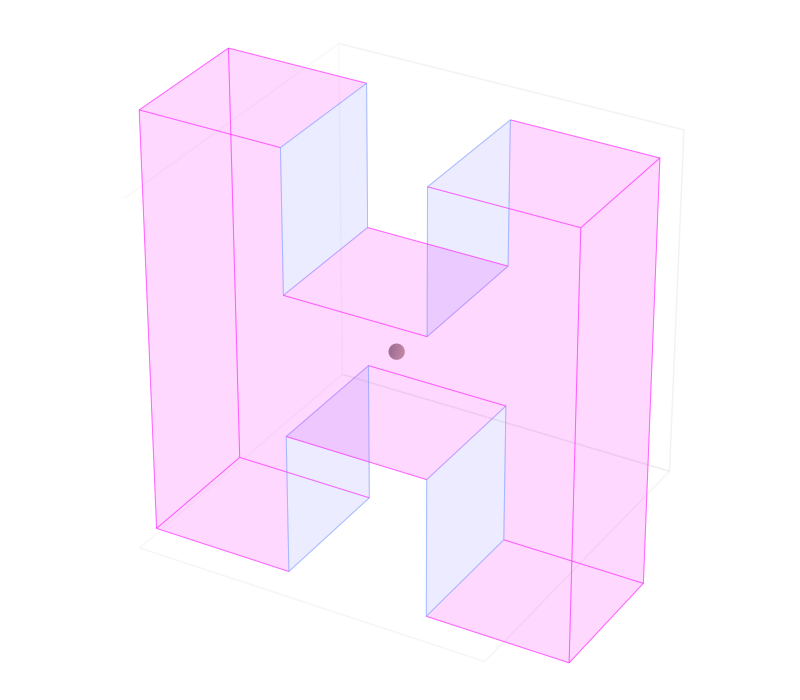
\includegraphics[width=0.4\textwidth]{figures/active_planes_for_hbox.png}
  \caption{All active faces (magenta) of the H-box container for
  point $c = (1.5, 0.5, 1.5)$ inside the container.}
  \label{fig:active_planes_inside}
\end{figure}

\begin{figure}[h!]
  \centering
  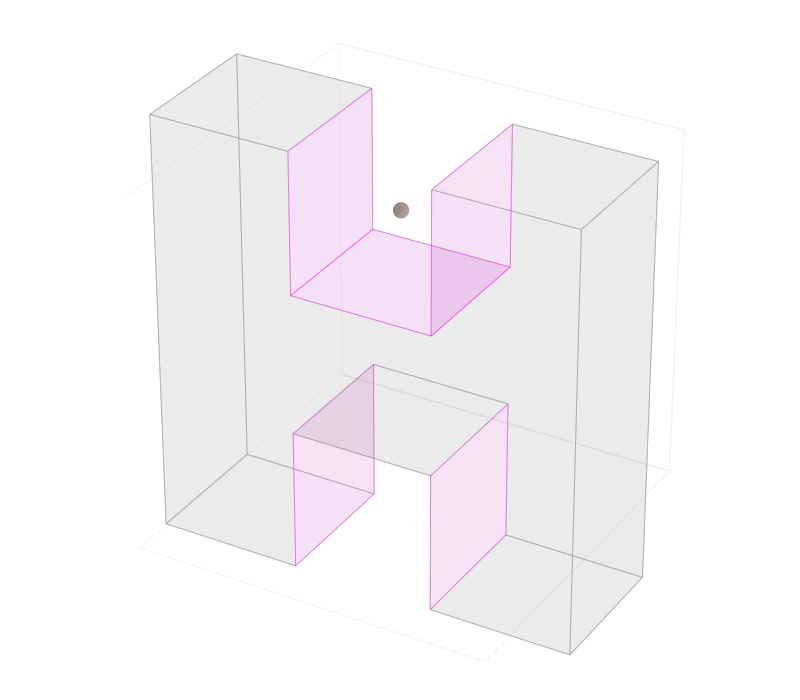
\includegraphics[width=0.4\textwidth]{figures/active_planes_for_hbox2.png}
  \caption{All active faces (magenta) of the H-box container for
  point $c = (1.5, 0.5, 2.5)$ outside the container.}
  \label{fig:active_planes_outside}
\end{figure}

Fig.~\ref{fig:active_planes_inside} depicts the active faces for a
point inside the H-shaped container, and
Fig.~\ref{fig:active_planes_outside} depicts the active faces for a
point outside the H-shaped container. An active face is a face whose
plane is relevant to the point $c$. If $c$ lies inside the container, the
active faces are those that have $c$ on their inward side. If $c$ lies
outside the container, an active face is one that has $c$ on its outward
side, between $c$ and the interior. Active faces contribute to the
boundary term of the feasibility-residual function.

\textbf{Active footpoint.} Consider a dispersion point $c$ and an
active face $F$ of the container $C$, and let $P$ be the plane through
$q_F$ with normal $N_F$. A \textit{foot} of $c$ on $P$ is a nearest point
of $P$ to $c$ in the metric $d$; by Equation~\ref{eq:plane} every foot
lies at distance $\abs{\ang{N_F, c - q_F}} / \norm{N_F}_*$ from $c$. We
say $c$ has an \textit{active footpoint} $w$ with respect to $F$ if some
foot of $c$ on $P$ lies on $F$, and we take $w$ to be such a foot. We
denote by $H^i$ the set of all active footpoints of the dispersion point
$c_i$.

Under the Euclidean metric the foot is unique and equals the orthogonal
projection of $c$ onto $P$, which recovers the construction of
\citet{lai2024}. Under a general norm the foot need not be unique, which is
why the definition only asks that \emph{some} foot lie on $F$. All feet of
$c$ on $P$ are at the same distance from $c$, so the distance an active
footpoint contributes does not depend on which foot we pick. What could
depend on the choice is whether that foot lies on $F$, and so whether $F$
contributes to the penalty at all. Asking only that some foot lie on $F$
removes this dependence: whether $c$ has an active footpoint on $F$ is
determined by $c$ and $F$ alone. Lemma~\ref{lem:zero} relies on this.

\begin{figure}[h!]
  \centering
  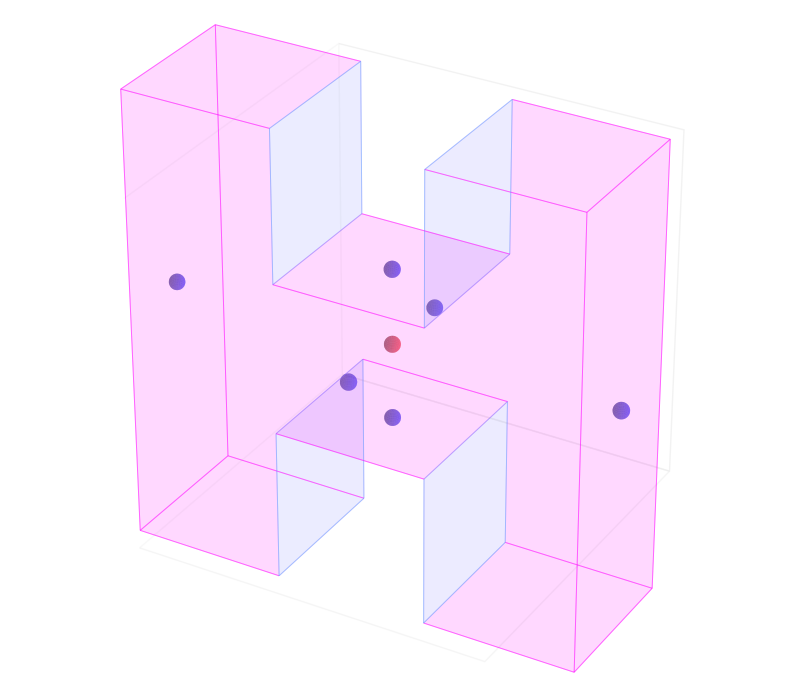
\includegraphics[width=0.4\textwidth]{figures/active_footpoints_in_hbox.png}
  \caption{All active footpoints (blue) inside the H-box container
    with respect to (red) point $(1.5, 0.5, 1.5)$ inside container with
  active faces highlighted in pink.}
  \label{fig:footpoints_inside}
\end{figure}

\begin{figure}[h!]
  \centering
  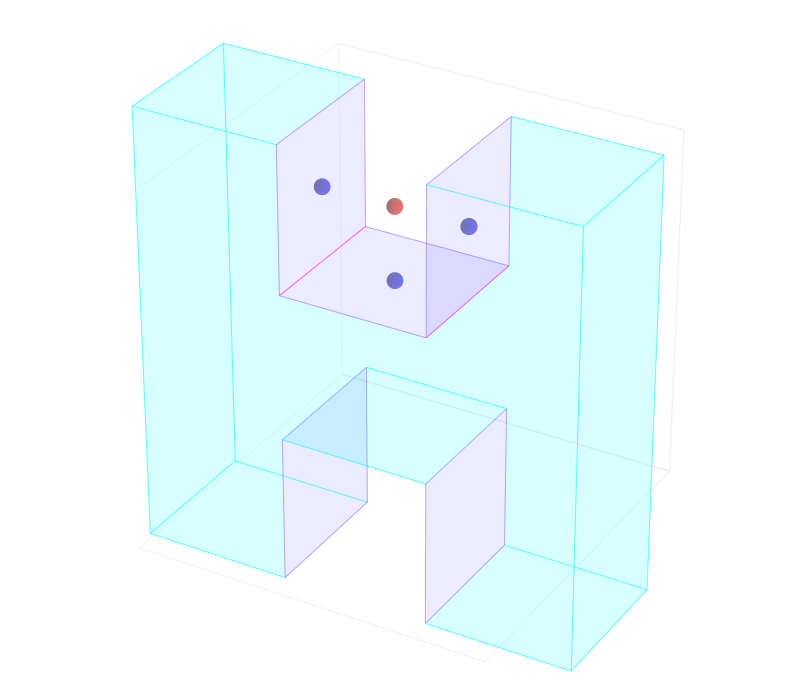
\includegraphics[width=0.4\textwidth]{figures/active_footpoints_in_hbox2.png}
  \caption{All active footpoints (blue) inside the H-box container
    with respect to (red) point $(1.5, 0.5, 2.5)$ outside container
  with active faces highlighted in purple.}
  \label{fig:footpoints_outside}
\end{figure}

Fig.~\ref{fig:footpoints_inside} depicts a case where the footpoints
of a dispersion point are all active.
Fig.~\ref{fig:footpoints_outside} depicts a case where not all
footpoints of a dispersion point are active. The active footpoints of a
dispersion point $c$ let us measure the distance from $c$ to the planes
of its active faces, and so to the boundary of the container. When a
nearest point of $P$ lies on the face $F$, the distance from $c$ to $F$ is
the distance from $c$ to this footpoint. When no nearest point of $P$ lies
on $F$, the nearest point of $F$ lies on the boundary of $F$ within its
plane, that is, on one of the edges of $F$. The penalty then accounts for
that part of the boundary through the edge set $\mathcal{E}$ rather than
through $H^i$.

The inward normals make the active-face rule a three-dimensional
counterpart of the counterclockwise active-edge rule of the planar
formulation \citep{lai2024}. In two dimensions the boundary is a closed
loop of segments with a natural cyclic order; the boundary of a
three-dimensional container has no such order. Active faces and their
footpoints extend the treatment of the boundary from vertices and edges in
two dimensions to vertices, edges and faces in three, and they apply in
the same way to every polyhedral container.

Now, we define the boundary penalty for a dispersion point $c_i$ as
\begin{equation}
  O_i =
  \begin{cases}
    \paren{D + 2 \min \set{d(c_i, v) : v \in \mathcal{V} \cup H^i}}^2 & c_i
    \notin C, \\[4pt]
    \displaystyle\sum_{v \, \in \, \mathcal{V} \, \cup \, \mathcal{E} \, \cup \, H^i}
    \paren{\max \set{0,\ D - d(c_i, v)}}^2 & c_i \in C.
  \end{cases}
  \label{eq:O_i}
\end{equation}
When $c_i \in C$, each vertex, edge and active footpoint contributes the
square of the amount by which its distance from $c_i$ falls below $D$.
The penalty is zero exactly when the open ball $B^o_D(c_i)$ meets no
vertex, edge or active footpoint of the container, and otherwise grows
with how far these features reach into the ball. A feature farther than
$D$ from $c_i$ contributes nothing.

The exterior branch minimizes over $\mathcal{V} \cup H^i$ only. Leaving out
the edges does no harm there. Outside the container the penalty is never
zero, so it does not need to measure the distance to the boundary exactly;
it only needs to be positive and to point back toward the container, and
$\mathcal{V} \cup H^i$ already gives such a direction. Inside the
container the edges are needed, because they cover the case in which no
foot of $c_i$ lands on its face (see the proof of Lemma~\ref{lem:zero}).

When $c_i \notin C$, the point violates the containment constraint
(\textit{i}), and $O_i$ is positive for every $D$. The squared form is at
least $D^2 > 0$, and it grows with the distance from $c_i$ to the nearest
vertex or active footpoint, so its gradient pushes an exterior point back
toward the container. A constant exterior penalty would also be positive,
but its gradient would be zero, so it would not move the point. The factor
$2$ sets the strength of that pull. Any positive factor gives the same zero
set (Lemma~\ref{lem:zero}); with $2$, the slope at the wall, $4D$, is twice
that of the interior branch, so a point that has left the container is
pulled back more strongly than a point inside is pushed from the wall.

We now define the energy function $E: (\R^3)^p \times \R \to \R$ of a
configuration $X = (c_1, \dots, c_p) \in (\R^3)^p$ and a radius $D$ by
\begin{equation}
  E(X, D) = \sum_{1 \le i < j \le p} \ell_{i, j}^2 + \sum_{i = 1}^p O_i.
  \label{eq:E}
\end{equation}

\begin{lemma}\label{lem:zero}
  \textit{For fixed $D > 0$, $O_i = 0$ if and
    only if $c_i \in C$ and $d(c_i, \partial C) \ge D$. Consequently
    $E(X, D) = 0$
  if and only if $(X, D)$ is feasible.}

  \textit{Proof.} If $c_i \notin C$ then $O_i \ge D^2 > 0$. Suppose $c_i \in
  C$. Every term of the interior branch vanishes exactly when $d(c_i, v) \ge D$
  for all $v \in \mathcal{V} \cup \mathcal{E} \cup H^i$, so it suffices to prove the
  covering identity
  \begin{equation}
    \min_{v \, \in \, \mathcal{V} \, \cup \, \mathcal{E} \, \cup \, H^i} d(c_i, v)
    = d(c_i, \partial C).
    \label{eq:covering}
  \end{equation}
  Each feature on the left is a subset of $\partial C$, so the left side is at
  least the right. For the reverse inequality, $\partial C$ is compact, so
  $d(c_i, \partial C) = d(c_i, y^*)$ for some $y^* \in \partial C$. If $y^*$
  lies on an edge $e$ of the container (in particular, if it is a vertex),
  then $d(c_i, e) \le d(c_i, y^*)$ and we are done. Otherwise $y^*$ lies in
  the relative interior of some face $F$, with plane $P$.

  We first show that $F$ is active. Suppose not. Then $\ang{N_F, c_i - q_F}
  < 0$, so $c_i$ lies strictly on the outward side of $P$, and $c_i \ne y^*$.
  Near $y^*$ the container lies on the inward side of $P$, so a point $w$ of
  the segment from $y^*$ to $c_i$, close enough to $y^*$ and different from
  it, is not in $C$. Let $z$ be the point of $C$ on the segment from $c_i$ to
  $w$ that is closest to $w$; it exists because $C$ is closed and $c_i \in C$.
  The points between $z$ and $w$ are not in $C$, so $z \in \partial C$. As
  $z$ lies on the segment from $c_i$ to $w$, and $w$ lies strictly between
  $c_i$ and $y^*$, homogeneity of the norm gives $d(c_i, z) \le d(c_i, w) <
  d(c_i, y^*)$, contradicting the choice of $y^*$. So $F$ is active.

  Next, $y^*$ minimizes $d(c_i, \cdot)$ over $\partial C$, hence over $F$, and
  $F$ contains a neighborhood of $y^*$ in $P$. So $y^*$ is a local minimizer of
  the convex function $y \mapsto d(c_i, y)$ on the plane $P$, hence a global
  one: $y^*$ is a foot of $c_i$ on $P$, and it lies on $F$. Therefore $c_i$
  has an active footpoint on $F$, which belongs to $H^i$ and, like every foot,
  lies at distance $d(c_i, P) = d(c_i, y^*) = d(c_i, \partial C)$ from $c_i$.
  In either case the left side of Equation~\ref{eq:covering} is at most
  $d(c_i, \partial C)$, which proves the identity. Hence, for $c_i \in C$,
  $O_i = 0$ exactly when $d(c_i, \partial C) \ge D$, which is constraint
  (\textit{iii}).

  The first term of Equation~\ref{eq:E} vanishes precisely when $d(c_i, c_j)
  \ge 2D$ for all $i \ne j$, which is constraint (\textit{ii}). Both terms are
  non-negative, so their sum vanishes only when each does.
  \hfill $\square$
\end{lemma}

The first term of Equation~\ref{eq:E} deals with the dispersion
constraint (\textit{ii}) of the CpDP, and the second term with the containment
and boundary constraints (\textit{i}) and (\textit{iii}). When $D$ is fixed, we
write $E_D(X) := E(X, D)$; this is the function Tabu Search minimizes
(Section~\ref{sec:tabu}).

Throughout, the quantity we report is the \emph{radius} $D$, not the minimum
separation $2D$. Constraint (\textit{ii}) asks for a distance of $2D$
between points, while constraint (\textit{iii}) asks for only $D$ between a
point and the boundary, because $D$ is the radius of a ball centered at each
dispersion point. Two such balls do not overlap when their centers are $2D$
apart, and a ball stays inside the container when its center is at
distance $D$ from the boundary. A configuration reported at radius $D$
therefore has minimum pairwise distance $2D$, and our comparisons against
sphere-packing tables \citep{packomania, schaer1966} are radius to radius.

Equation~\ref{eq:E} gives a feasibility-residual function which lifts
the optimization model proposed by \citet{lai2024} from two
dimensions into three dimensions. It is also differentiable almost
everywhere on $(\R^3)^p \times \R_{>0}$. The value of $E$ depends on a few
discrete choices for each point $c_i$: whether $c_i \in C$, which faces are
active, and on which active faces $c_i$ has a footpoint. Let $Z$ be the set
of $(X, D)$ at which some $c_i$ lies on $\partial C$, on the plane of some
face, or on the boundary of the set of points that have a footpoint on a
given face. For a polyhedral norm the last of these sets is a finite union
of polyhedra, and for $\ell_2$ it is a prism over the face, so in every case
its boundary lies in finitely many planes. Hence $Z$ is contained in finitely
many sets of the form $\set{(X, D) : c_i \in \Pi}$ with $\Pi$ a plane, and
has measure zero. Off $Z$ every discrete choice is constant on a
neighborhood, and there $E$ is a finite sum of terms $g(2D - d(c_i, c_j))$,
$g(D - d(c_i, S))$ and $\paren{D + 2 \min_k d(c_i, S_k)}^2$, where each $S$
and $S_k$ is a fixed vertex, edge or face plane. Each term is locally
Lipschitz by Lemma~\ref{lem:lipschitz}, so $E$ is locally Lipschitz off $Z$
and differentiable almost everywhere there by Rademacher's Theorem. As $Z$
has measure zero, $E$ is differentiable almost everywhere, which permits the
use of gradient-based solvers such as L-BFGS-B \citep{byrd1995}.

$E$ is not continuous everywhere. Inside the container, when the footpoint
of $c_i$ on a face reaches an edge of that face, the footpoint and the edge
are at the same distance $\delta$ from $c_i$, so if $\delta < D$ both
contribute $(D - \delta)^2$; once the footpoint leaves the face, only the
edge term remains, and $E$ drops by $(D - \delta)^2$. Similarly, as $c_i$
approaches the boundary from inside near an edge or a vertex, the interior
branch tends to a sum over every feature within $D$ of $c_i$, which exceeds
the value $D^2$ that the exterior branch takes on the other side of the
wall. These jumps lie in the measure-zero set $Z$, so they do not affect
almost-everywhere differentiability, but a line search may meet them.
Replacing the interior sum by $\paren{\max \set{0, D - \min_v d(c_i,
v)}}^2$, which by Equation~\ref{eq:covering} equals $g(D - d(c_i,
\partial C))$, removes the jump inside the container and has the same zero
set, so Lemma~\ref{lem:zero} still holds; the exterior branch can still
jump, because the set of active footpoints changes as $c_i$ moves outside
the container. In preliminary runs on four cells the sum gave equal or
slightly larger best radii and the minimum gave larger mean radii, so
neither dominated, and we keep the sum.

Both $E$ and the penalty function $\Phi_\mu$ of Section~\ref{sec:adjust}
(Equation~\ref{eq:phi_mu}) are differentiated in closed form rather than by
finite differences. The dispersion term $\ell_{i, j}^2$ contributes $-2
\ell_{i, j} \, \partial d(c_i, c_j) / \partial c_i$ to the gradient with
respect to $c_i$, and $4 \ell_{i, j}$ to the derivative with respect to $D$. The vertex and
footpoint terms differentiate the norm directly, using a
\emph{subgradient} of the norm at the displacement $z = c_i - v$: a vector
$s$ with $\norm{y} \ge \norm{z} + \ang{s, y - z}$ for all $y$, which is the
gradient wherever the norm is differentiable \citep{boyd2004}. For $\ell_2$,
$s = z / \norm{z}_2$; for a polyhedral norm, $s = g_{k^*}$ with $k^*$
attaining the maximum in Equation~\ref{eq:gen}. The edge terms use the
segment gradient of Section~\ref{sec:polyhedral}. The face terms use
$\partial \paren{\abs{h} / \norm{N_F}_*} / \partial c_i = \mathrm{sgn}(h)
N_F / \norm{N_F}_*$, where $h = \ang{N_F, c_i - q_F}$ as in
Equation~\ref{eq:plane}; this does not depend on which foot the face
contributes. The derivatives of $E$ and $\Phi_\mu$ with respect to $D$ are
accumulated in the same pass, so one pass returns $\Phi_\mu$, $\nabla_X
\Phi_\mu$ and $\partial \Phi_\mu / \partial D$ together.

Closed-form gradients matter for two reasons. First, a finite-difference
gradient over the $3p + 1$ variables costs that many extra evaluations of
$E$, or twice that for central differences, while the closed form needs a
single pass. On the unit cube the analytic gradient is 20 times faster than
central differences at $p = 10$ and 185 times faster at $p = 60$, and the
gap widens with $p$ as the number of perturbations predicts. Second, a
difference step interacts badly with a function that is only
differentiable almost everywhere: a step that crosses a kink returns a
slope that belongs to neither side.

\section{Global Optimization Algorithm}

In this section we propose our global optimization algorithm which
builds upon the framework introduced by \citet{lai2024}. The global
optimization process is structured as a multi-start pipeline to
navigate the complex, non-convex solution space. In each global
iteration, the algorithm restarts by generating an initial random
configuration of $p$ points uniformly distributed within the
polyhedral container. This multi-start approach is necessary because
the problem’s non-smooth objective function and numerous distance
constraints frequently trap standard optimization tools in poor local
optima \citep{dai2021}. As shown in
Fig.~\ref{fig:tabu_search_overview}, within each iteration, the Tabu
Search procedure acts as a feasibility solver: it minimizes the
feasibility-residual function of Equation~\ref{eq:E} to find a feasible
configuration for a fixed radius $D$. Once a feasible
configuration is found, a distance adjustment procedure applies the
Sequential Unconstrained Minimization Technique (SUMT)
\citep{fiacco1964} to iteratively maximize $D$ while preserving the
feasibility of the configuration.

\begin{figure}[h!] % or [htbp] for flexible placement
  \centering
  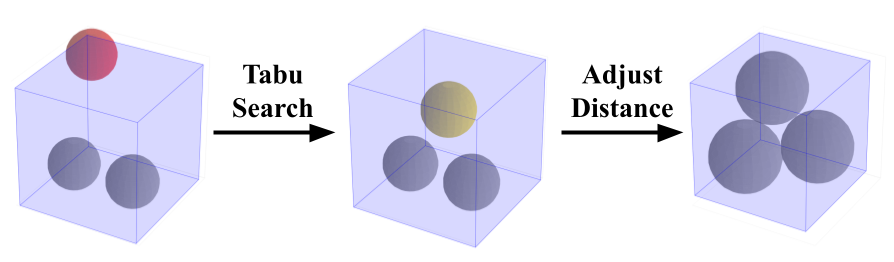
\includegraphics[scale=0.25]{figures/global_optimization_algorithm_visualization.png}
  \caption{Overview of the global optimization algorithm. The process
    demonstrates a two-stage approach: first, Tabu Search is employed
    to relocate a candidate sphere (red) from an initial, infeasible
    position to a feasible position (yellow). Second, an Adjust
    Distance phase maximizes the uniform radius of all spheres to
  achieve an optimal packing configuration.}
  \label{fig:tabu_search_overview}
\end{figure}

\subsection{Tabu Search}\label{sec:tabu}

We employ a Tabu Search procedure \citep{glover1997}, following the
framework used by \citet{lai2024}. Tabu Search is a combinatorial
heuristic designed to escape poor local configurations (high-energy)
and move the system toward a better (lower-energy) arrangement of
dispersion points inside the container. The core principle behind the
Tabu Search is the \textit{tabu list}, a short-term memory of recent
moves that are forbidden for a number of subsequent iterations
\citep{glover1997}. The tabu list keeps the algorithm from cycling
through the same configurations.

A move in our setting relocates a point to a position in $\R^3$, and a
continuous position never recurs exactly, so a list keyed on positions would
forbid nothing. We therefore key an entry on the pair (index of the moved
point, cell of a grid of side $\delta = D/20$ containing its destination),
so two moves count as the same if they send the same point into the same
small cell. Tying $\delta$ to $D$ rather than to the container keeps the
resolution of the memory proportional to the size of the balls.

Each accepted move adds two entries: its own pair, and the pair of the same
point with the cell it left. A candidate move of a point is forbidden if the
list holds that point paired with either its destination cell or the cell
it currently occupies. A point that has just been moved can therefore
neither return to the cell it left nor move on, until the entries lapse.
Entries expire two ways: each lapses seven iterations after it is added,
so it forbids moves for the next six, and the list holds at most $20$
entries, the oldest being evicted when it overflows. Finally, the
prohibition is subject to an \textit{aspiration criterion}: a forbidden
move is taken anyway if it yields a configuration strictly better than the
best seen so far.

The Tabu Search heuristic incentivizes long-term exploration of the
solution space. The maximum number of successive moves the algorithm
is allowed to explore without improving from the initial
configuration is specified by a parameter $\beta$. If Tabu Search
makes $\beta$ iterations without improving on the last-improved
configuration, then the procedure terminates. A small $\beta$ enables
a quicker Tabu Search, but only scans for solutions which are a few
moves different from the initial configurations. A large $\beta$
enables a deeper scan of neighboring solutions, but forces a longer
runtime for Tabu Search.

We quantify the \textit{energy of a point} by how much it violates the
dispersion and boundary constraints, with the other points held fixed.
We define the energy of a dispersion point $c_i$ as
\begin{equation}
  E_D(c_i) = \sum_{j \ne i} \ell_{i, j}^2 + O_i
  \label{eq:dispersion_point_energy}
\end{equation}
where $\ell_{i, j}$ is the dispersion penalty term and $O_i$ captures
the boundary violation term as in Equation~\ref{eq:O_i}. To propose
new candidate positions for dispersion points, we consider
\textit{vacancy sites}, which are random locations inside the
container not currently occupied by a dispersion point. A vacancy
site $c$ has energy
\begin{equation}
  E_D(c) = \sum_{j = 1}^p \ell_{c, j}^2 + O_{c}
  \label{eq:vacancy_energy}
\end{equation}
where $\ell_{c, j}$ replaces $c_i$ with $c$ in Equation~\ref{eq:lij}
and $O_c$ replaces $c_i$ with $c$ in Equation~\ref{eq:O_i}. Vacancy
sites with low energy represent positions that are more compatible
with the current configuration, i.e., points where it would be the
``easiest'' to insert another ball.

A \textit{neighbor} $X_{nb}$ of a solution $X$ can be found by
\textit{moving} a single dispersion point of $X$ to a new location.
The \textit{neighborhood} $N(X)$ is the set of neighbors of $X$. To
select the most promising neighbor of a given configuration $X$, we
sample $N(X)$ by identifying the $Q$ highest-energy dispersion points
and the $Q$ lowest-energy vacancy sites selected from a pool of $10p$
randomly generated candidates, where $p$ is the total number of
dispersion points. While \citet{lai2024} suggest generating only $5p$
vacancy sites, we increased this sample size to $10p$ to maintain
sufficient search breadth, compensating for the lower sampling
density inherent in three-dimensional space. We
analyze the possible moves between these sets to identify the pairing
that offers the best potential reduction in energy.

For a specific dispersion-vacancy move, the resulting configuration
is merely a rough approximation of a feasible solution. Since vacancy
sites are generated randomly, simply placing a point at one of these
coordinates rarely resolves the feasibility-residual value, defined
in Equation~\ref{eq:E}, to zero. Therefore, we do not evaluate the
quality of this raw move directly. Instead, we pass this intermediate
configuration to our local optimization subroutine,
\textsc{LocalOpt}, which connects the discrete moves of Tabu Search to
the continuous problem. It runs L-BFGS-B \citep{byrd1995} on the energy,
for at most $100$ iterations, to take the rough candidate configuration to a
nearby local minimum.
Consequently, the Tabu Search algorithm never compares unrefined
moves; it strictly compares the \textit{locally optimized} outcomes
of those moves to decide if a step is an improvement.

\begin{rvdraft}
However, even with this precise local refinement, the global solution
space of Equation~\ref{eq:E} remains non-convex and populated with
numerous local minima \citep{lai2024}. To prevent the algorithm from
becoming trapped in the first deep valley it encounters, we integrate
Monotonic Basin Hopping (\textsc{MBH}) as a heuristic for global
exploration, as suggested by \citet{lai2024}. Unlike Tabu Search,
which evolves a solution along a specific path, \textsc{MBH} samples
the global landscape by ``hopping'' between independent basins (i.e.,
regions converging to a single minimum) \citep{back2013}. It operates
by taking a solution $(c_1, \dots, c_p, D)$, perturbing it at random to
jump into a neighboring basin, and then minimizing the residual locally
with L-BFGS-B. We run
ten such hops per call. Each hop moves every coordinate by up to $D$, so
the step size scales with the radius rather than with the container. A
hop is kept only if the residual does not increase, so \textsc{MBH} never
makes the configuration it is given worse. A variant that also accepts
hops that increase the residual can cross barriers between basins that
ours cannot. \rvclaim{In our tests (cube and star, $p = 100$, $\ell_2$, four
seeds) this variant did not reach the best basin more often than ours on
the cube, and reached it less often on the star}. Configurations that
monotone hops cannot leave are handled instead by the escape step of
Section~\ref{sec:global}.
\end{rvdraft}

\textsc{MBH} is applied inside the Tabu Search loop rather than as a
separate outer layer, on the configuration that results from taking the
chosen move (line~\ref{line:mbh} of Algorithm~\ref{alg:tabu_search}). The two
heuristics address different failure modes: the tabu memory prevents the search from re-taking a move it has just
undone, while \textsc{MBH} perturbs whatever configuration that move
produced. Placing it outside the loop would leave each tabu iteration to
terminate in its own basin with no means of leaving it.

\begin{algorithm}[H]
  %\SingleSpacedXI % <--- INFORMS-specific single spacing command
  \caption{Tabu Search}
  \begin{algorithmic}[1]
    \Require $C$ (Container), $X$ (configuration), $D \in \R_{> 0}$,
    $\beta \in \Z_{> 0}$, $Q \in \Z_{> 0}$, $\epsilon \in \R_{> 0}$
    \State $Q \gets \min \set{Q, p}$
    \State $X \gets \textsc{LocalOpt}(X, D)$
    \State $X^{\text{best}} \gets X$, $\emph{NoImprove} \gets 0$,
    $\emph{TabuList} \gets \set{}$
    \While{$\emph{NoImprove} \le \beta$ and $E_D(X^{\text{best}}) > \epsilon$}
    \State $p_1, \dots, p_Q \gets \textsc{HighEnergyPoints}(X, D, Q)$
    \State $q_1, \dots, q_Q \gets \textsc{VacancySites}(X, D, Q)$

    \State $X^{\text{best}}_{\text{nb}} \gets X$,
    $e^{\text{best}}_{\text{nb}} \gets \infty$,
    $\emph{BestMove} \gets \textsc{Nil}$
    \For{$(i, j) \in [Q] \times [Q]$}
    \State $X_{\text{nb}} \gets
    \textsc{LocalOpt}(\textsc{MovePoint}(X, p_i, q_j), D)$
    \State $a \gets \left(\textsc{Move}(p_i, q_j) \text{ not forbidden}\right)$
    \textbf{or} $\left(E_D(X_{\text{nb}}) < E_D(X^{\text{best}})\right)$
    \If {$a$ \textbf{and} $E_D(X_{\text{nb}}) < e^{\text{best}}_{\text{nb}}$}
    \State $X^{\text{best}}_{\text{nb}} \gets X_{\text{nb}}$,
    $e^{\text{best}}_{\text{nb}} \gets E_D(X_{\text{nb}})$
    \State $\emph{BestMove} \gets \textsc{Move}(p_i, q_j)$
    \EndIf
    \EndFor
    \If{$\emph{BestMove} \ne \textsc{Nil}$}
    \State $X \gets X^{\text{best}}_{\text{nb}}$
    \State Add $\emph{BestMove}$ and its reverse to \emph{TabuList}
    \EndIf
    \State $X \gets \textsc{MBH}(X, D)$ \label{line:mbh}
    \If{$E_D(X) < E_D(X^{\text{best}})$}
    \State $X^{\text{best}} \gets X$

    \State $\emph{NoImprove} \gets 0$
    \Else
    \State $\emph{NoImprove} \gets \emph{NoImprove} + 1$
    \EndIf
    \EndWhile
    \State \Return $X^{\text{best}}$
  \end{algorithmic}
  \label{alg:tabu_search}
\end{algorithm}

Algorithm~\ref{alg:tabu_search} outlines the Tabu Search procedure.
To visualize the effect of Tabu Search, Fig.~\ref{fig:tabu_search}
illustrates a candidate move for a fixed radius $D$ within a cubic container.

The dispersion point shown in red is in a high-energy state due to a
boundary constraint violation (protrusion from the container). The
yellow sphere represents a randomly generated vacancy site located in
a feasible region. The red arrow indicates the proposed movement:
displacing the violating particle to this vacancy site. In this
specific example, because the target site satisfies all constraints
(it is inside the boundary and non-overlapping), the
feasibility-residual value is zero. Consequently, the subsequent
\textsc{LocalOpt} routine will confirm this new configuration as
stable with minimal energy. To prevent cycling, the algorithm explicitly
forbids the reverse move in future iterations; the yellow dispersion
point is temporarily restricted from returning to the high-energy
neighborhood of the red sphere. This demonstrates the primary
function of Tabu Search: executing coarse, global jumps to locate
feasible regions, which are then refined by local optimization.

\begin{figure}[h!] % or [htbp] for flexible placement
  \centering
  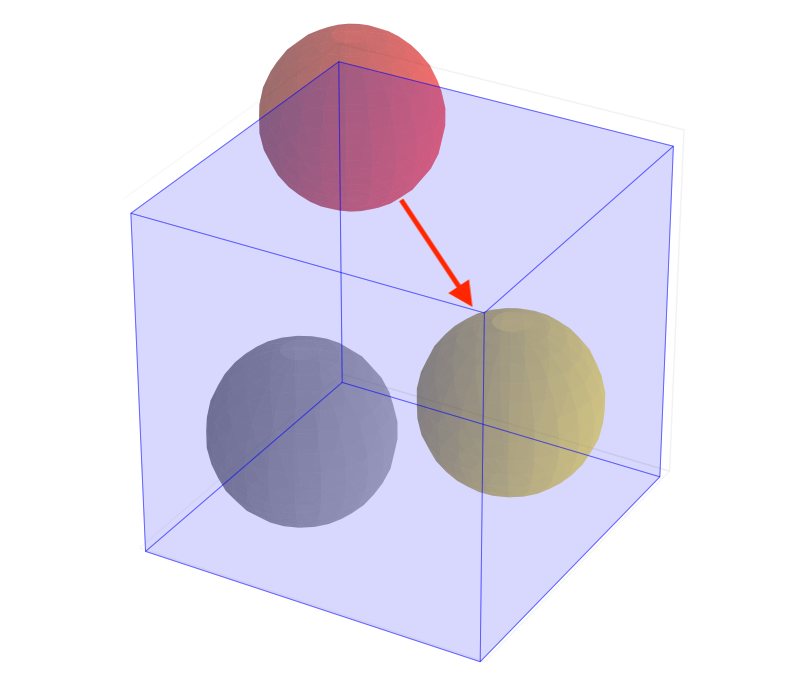
\includegraphics[scale=0.2]{figures/tabu_search.png}
  \caption{\textbf{Visualization of a candidate neighbor generation.}
    The red sphere represents the point selected for movement (e.g., a
    high-energy point). The red arrow indicates the proposed
    displacement vector, targeting the location currently occupied by
  the yellow sphere.}
  \label{fig:tabu_search}
\end{figure}

\subsection{Adjust Distance}\label{sec:adjust}

After the Tabu Search procedure is completed, the resulting
configuration $X$ is a feasible solution, but typically not optimal.
To move $X$ to a nearby local optimum $X^*$, we employ the Sequential Unconstrained
Minimization Technique (SUMT) \citep{fiacco1964} as proposed by
\citet{lai2024} to convert the original CpDP (as a constrained
optimization problem) into a sequence of unconstrained optimization
problems and solve each until a feasible local minimum solution is
found. Each unconstrained subproblem can be expressed as
\begin{equation}
  \textit{Minimize} \quad \Phi_\mu(X, D) = -D^2 + \mu \times E(X, D)
  \label{eq:phi_mu}
\end{equation}
where $X$ is a candidate solution, $D$ is the radius of the solution
$X$, $\mu$ is the penalty factor to define the unconstrained
optimization problem.

Algorithm~\ref{alg:adjust_distance} is the method to adjust a
feasible configuration from Algorithm~\ref{alg:tabu_search} into a
local optimum. The distance adjustment method will iteratively
minimize Equation~\ref{eq:phi_mu} for strictly increasing values of
$\mu$. The $-D^2$ term in Equation~\ref{eq:phi_mu} is to ensure that
when we minimize this function, we promote maximizing $D$.
Equation~\ref{eq:O_i} contains $(\max\set{0, D - d(c_i, v)})^2$ which
grows quadratically with $D$. The $-D^2$ term thus ensures
Equation~\ref{eq:phi_mu} is not dominated by $E(X, D)$
\citep{lai2024}. The distance adjustment procedure slightly adjusts
the configuration $X$ and the allowed minimum distance $D$ through
local optimization to find a local optimum of the original CpDP.

\begin{algorithm}[H]
  %\SingleSpacedXI % <--- INFORMS-specific single spacing command
  \caption{Adjust Distance}
  \begin{algorithmic}[1]
    \Require $X_0$ (configuration), $D_0 \in \R_{> 0}$, $K \in \Z_{> 0}$,
    $\epsilon \in \R_{>0}$, $\mu_{\mathrm{s}} \in \R_{>0}$ (default $1$)
    \State $X \gets X_0$, $D \gets D_0$, $\mu \gets \mu_{\mathrm{s}}$
    \For{$i \gets 1$ to $K$}
    \State $\mu \gets 10 \cdot \mu$
    \State $(X, D) \gets \textsc{LocalOptPhi}(X, D, \mu)$
    \If{$(X, D)$ unchanged for three consecutive iterations}
    \State \textbf{break}
    \EndIf
    \EndFor
    \If{$E_D(X) \ge \epsilon$}
    \Comment{infeasible: snap to the exact bound}
    \If{$B(X) > 0$}
    \State $D \gets \min \set{0.95 D,\ B(X)}$
    \Else
    \State $D \gets 0.95 D$
    \EndIf
    \State $X \gets \textsc{LocalOpt}(X, D)$
    \State $(X, D) \gets \textsc{AdjustDistance}(X, D, 5, \epsilon, 10^3)$
    \EndIf
    \If{$B(X) > 0$}
    \State $D \gets B(X)$
    \Comment{exactly what $X$ supports}
    \EndIf
    \State \Return $(X, D)$
  \end{algorithmic}
  \label{alg:adjust_distance}
\end{algorithm}

The \textsc{LocalOptPhi} function is a run of L-BFGS-B on the function
$\Phi_\mu$ from an initial solution $(X, D)$ and penalty factor $\mu$,
with the bound $D \ge 0$. With $\mu_{\mathrm{s}} = 1$ and $K = 15$, $\mu$ is
multiplied by $10$ before each subproblem, so the schedule runs from $10$ to
$10^{15}$. A larger starting $\mu$ makes the first gradient ill-conditioned:
the penalty term then dominates $-D^2$ from the outset, and the first iterate
is driven to satisfy the constraints at whatever radius it starts from rather
than trading radius against violation. Starting small and multiplying
lets each iteration begin near the previous minimizer.

The procedure relies on the bound
\begin{equation}
  B(X) = \min \set{\min_{i < j} \tfrac{1}{2} d(c_i, c_j),\ \min_i d(c_i,
  \partial C)},
  \label{eq:bound}
\end{equation}
the largest radius that the configuration $X$ supports. If every point of
$X$ lies in $C$, then $(X, D)$ is feasible exactly when $0 < D \le B(X)$:
constraint (\textit{ii}) requires $D \le \tfrac12 d(c_i, c_j)$ for every
pair of points, and constraint (\textit{iii}) requires $D \le d(c_i,
\partial C)$ for every point. Every $D$ we report is set from $B(X)$ for
the reported configuration, so it is feasible by construction rather than
up to a tolerance.

Algorithm~\ref{alg:adjust_distance} uses $B(X)$ in two places. First, if
SUMT ends infeasible, $D$ is lowered to $\min \set{0.95 D, B(X)}$ in one
step, rather than in fixed proportional steps that could run out of
retries while still infeasible; if $B(X) = 0$, a point has left the
container and $D$ is lowered by $5\%$ instead. The retry then resumes the
penalty schedule at $\mu = 10^4$ rather than restarting it, since the
configuration it continues from is already close to feasible, and at most
five nested retries are made. Second,
whichever side of $B(X)$ SUMT stops on, the algorithm returns $B(X)$
itself. Returning the radius SUMT stops at would, from above, allow a
constraint violation of up to $\sqrt{\epsilon}$, since only $E < \epsilon$
is enforced, and from below, understate the radius. We return $B(X) (1 -
10^{-9})$, which leaves a small margin against rounding error in the final
evaluation. In practice $B(X) = 0$ only when a point has left the
container, and such a run is reported as infeasible.

Returning $B(X)$ also guards against a degenerate outcome. Whenever the
points are well separated, $D = 0$ is a \emph{stationary point} of
$\Phi_\mu$ on the bound $D \ge 0$, that is, a point at which the solver sees
no direction of descent: there $E = 0$ and $\partial \Phi_\mu / \partial D
= -2D = 0$. An overestimated $D_{\text{init}}$ can drive SUMT to this
trivially feasible answer, and resetting $D$ to $B(X) > 0$ recovers the
radius the configuration actually supports.

Note that \textsc{LocalOpt} is called in
Algorithm~\ref{alg:adjust_distance} only on the infeasible branch, where $D$
has just changed and minimizing $E_D(X)$ can therefore still help. It is not
called in the main loop, where $D$ is free and \textsc{LocalOptPhi} already
varies it. Conversely it would not help to call \textsc{LocalOptPhi} in
Algorithm~\ref{alg:tabu_search}, since Tabu Search is only designed for
finding feasible configurations at a fixed $D$. It is important not to
``rush'' finding a maximal value of $D$, as finding a stable and feasible
configuration $X$ first often leads to a smoother maximization of $D$.

\subsection{Global Optimization}\label{sec:global}

The global optimization procedure is summarized in
Algorithm~\ref{alg:global_opt}, a three-dimensional analogue of the
TSGO framework of \citet{lai2024}. \citet{lai2024} run a single search
that keeps building on the global best configuration until a time limit
is reached. Our algorithm instead makes independent restarts. Each
restart draws a new random configuration and runs Tabu Search at the best
radius found so far, $D^*$. A run stops when $R$ restarts in a row fail to
improve $D^*$, after $N$ restarts, or once the time limit $T$ has passed,
whichever comes first. Because every restart begins from a new random
configuration, it is not tied to a local optimum found earlier, which
matters most in non-convex containers whose feasible region may be
disconnected. When the run ends, \textsc{Polish} (Section~\ref{sec:results})
tightens the best configuration found.

\paragraph{Escape.}\label{sec:escape} A restart runs Tabu Search at $D^*$,
and Tabu Search moves points only while the residual is positive. A random
start that is already feasible at $D^*$ is therefore returned unmoved, even
if its points are badly placed, and a narrow feature of the container can
then hold a point in a poor position on every restart. So when a restart
ends feasible but does not raise $D^*$, we make one \emph{escape} attempt
from its configuration. Tabu Search is run again at $\gamma D^*$, with
$\gamma = 1.02$, where that configuration is infeasible and its points have
to move. \textsc{AdjustDistance} then adjusts the radius from wherever Tabu
Search leaves it: it grows the radius if that configuration is feasible, and
otherwise lowers it until the configuration is feasible
(Section~\ref{sec:adjust}). The result replaces the best only if it beats it,
and an escape that raises $D^*$ resets the patience counter like any other
improvement. The attempt runs inside the same time limit.

\begin{algorithm}[H]
  %\SingleSpacedXI % <--- INFORMS-specific single spacing command
  \caption{Global Optimization}
  \begin{algorithmic}[1]
    \Require $p \in \mathbb{N}$, $C$, $D_{\text{init}} \in \R_{>0}$, $N$ (most
    restarts), $R$ (patience), $T$ (time limit), $\gamma > 1$ (escape
    factor), $\epsilon \in \R_{> 0}$
    \Ensure Best configuration $(X^*, D^*)$

    \State $D \gets D_{\text{init}}$
    \State $X \gets \textsc{RandomSolution}(p)$
    \State $X \gets \textsc{TabuSearch}(X, D)$
    \State $X, D \gets \textsc{AdjustDistance}(X, D)$
    \State $X^*, D^* \gets X, D$
    \State $s \gets 0$

    \For {$i = 1$ \textbf{to} $N$}
    \If{$s \ge R$ \textbf{or} more than $T$ has elapsed}
    \State \textbf{break}
    \EndIf
    \State $s \gets s + 1$
    \State $X_i \gets \textsc{RandomSolution}(p)$
    \State $X_i \gets \textsc{TabuSearch}(X_i, D^*)$
    \If{$E_{D^*}(X_i) < \epsilon$}
    \State $(X_i, D_i) \gets \textsc{AdjustDistance}(X_i, D^*)$
    \State $\textsc{Accept}(X_i, D_i)$
    \If{$s > 0$} \Comment{no gain: escape}
    \State $X_i \gets \textsc{TabuSearch}(X_i, \gamma D^*)$
    \State $(X_i, D_i) \gets \textsc{AdjustDistance}(X_i, \gamma D^*)$
    \State $\textsc{Accept}(X_i, D_i)$
    \EndIf
    \EndIf
    \EndFor
    \State $(X^*, D^*) \gets \textsc{Polish}(X^*)$
    \State \Return $(X^*, D^*)$
  \end{algorithmic}
  \label{alg:global_opt}
\end{algorithm}

Every call to \textsc{AdjustDistance} uses $K = 15$. Here
$\textsc{Accept}(X_i, D_i)$ replaces $(X^*, D^*)$ by $(X_i, D_i)$ if
$D_i > D^*$ and $E_{D_i}(X_i) < \epsilon$, and resets $s$ to $0$ if moreover
$D_i > (1 + 10^{-7}) D^*$; so $s > 0$ after the first \textsc{Accept} exactly
when the restart gained nothing.

Within each iteration, the algorithm uses the same local search
operators as \citet{lai2024}. An initial configuration is generated by
\textsc{RandomSolution}, and \textsc{TabuSearch} then looks for a
feasible configuration at radius $D_i$. Only if the feasibility-residual
value $E_{D_i}(X_i)$ falls below the tolerance $\epsilon$ does the
algorithm proceed to \textsc{AdjustDistance}, so the more expensive
radius adjustment runs only on feasible configurations. At the local
level, every subroutine relies on a gradient-based solver applied to
Equation~\ref{eq:E}. Unlike repulsion-based heuristics, which simulate a
physical system, these solvers follow the gradient of an explicit
objective.

\section{Results and Evaluation}\label{sec:results}

\begin{rvdraft}
Experiments are run on \tbdtext{cluster CPU model, memory per core and
operating system}, one core per run. CPU times are given in seconds. The algorithm is
implemented in Python 3.11, and the source code is publicly available
(\href{https://github.com/leadcatlab/continuous-p-dispersion}{Source
Code}). The repository's \texttt{supplement} folder lists the centers of every
configuration we report, at full double precision, with each container's
faces and a standalone script, \texttt{verify\_packing.py}, that needs only
NumPy and none of our solver. From the centers alone it recomputes the
largest feasible radius exactly, in any of the three norms: half the smallest
pairwise distance, or the smallest distance from a center to a face, whichever
is less, with every center inside the container. For all \tbd{377}
configurations it agrees with the radius we report, which sits a relative $10^{-9}$ below it by
design. Our solver pairs Tabu Search with L-BFGS-B to handle the
problem's $3p+1$ variables and its highly non-convex solution space. We
enforce a constraint
violation tolerance of $\epsilon=10^{-8}$ and truncate reported
results to eight decimal places, ensuring the reported configurations
are strictly feasible within the container geometry.
\end{rvdraft}

We evaluate our algorithm on five polyhedral containers of increasing
geometric complexity (the unit cube, the regular tetrahedron of unit edge,
an H-shaped box, a star-shaped polyhedron and a ribbed ventilation cage)
and on the eight multi-connected domains of \citet{stoyan2013}
(Section~\ref{sec:stoyan}).
The boundaries for each are defined using a vectorized representation
of inward-pointing normals for efficient distance calculations. To
evaluate robustness, we benchmarked our algorithm against Packomania
records \citep{packomania}, the results of \citet{kazakov2018}, optimality
certificates from Gurobi \citep{gurobi2026}, and two general-purpose nonlinear
programming solvers, IPOPT \citep{wachter2006} and SLSQP \citep{kraft1988,
scipy2020}, run under an equal time budget. The protocol for that comparison
(solvers, formulations, cells, budgets and statistics) was fixed in writing
before any run, and is given in Section~\ref{sec:baselines}.

\begin{rvdraft}
Every run is Algorithm~\ref{alg:global_opt}: a first start from
$D_{\text{init}}$, then restarts from fresh random configurations at the best
radius found so far, until $R = \lceil 3 \ln p \rceil$ restarts in a row
(a rule chosen below) fail
to raise it by more than a relative $10^{-7}$, with at most $N = 40$ restarts
and $T = 30$ minutes per run, and with the escape step of
Section~\ref{sec:global} ($\gamma = 1.02$). A restart still running when the time limit
is reached is allowed to complete, so a run can exceed $T$. Tabu Search depth is $\beta = 10$ and the tabu-rearrangement
parameter is $Q = \max(3, \operatorname{round}(\ln p))$, which is the value
$Q = 3$ of \citet{lai2024} for $p \le 33$. Each cell (container, metric, $p$)
is run from $20$ independent seeds. The restarts are what put Tabu
Search to work. From a start at or below the initial estimate $\hat D$
(Equation~\ref{eq:dinit_of_rho} below), the first \textsc{LocalOpt} usually
reaches $E_D < \epsilon$ on its own, and Tabu Search then performs no
iterations at all. A restart at the best radius so far rarely does, so
there the search has to relocate points to find a feasible configuration.
We chose the number of restarts by replaying 160 long runs (cube, tetrahedron, H-box and star; $\ell_2$ and
$\ell_1$; $p = 10$ to $100$; capped at 41 starts or 30 minutes) against
stopping rules constant in $p$ and growing as $\ln p$, $\sqrt p$ and $p$:
\rvclaim{$\lceil 3 \ln p \rceil$ used $81\%$ of the capped CPU time, lost $0.003\%$ of
the radius on average, and lost more than $0.01\%$ in one cell of 40.} At large
$p$ the time limit binds first (Section~\ref{sec:runtime}). $Q$ grows with
$p$ because each Tabu Search iteration costs $Q^2$ local optimizations, so
at a fixed budget a larger $Q$ buys a wider search at the price of fewer
restarts, and the balance shifts with $p$. On the cube at $p = 100$, $Q = 5$
gave a larger mean, median, best and worst radius than $Q = 3$ or $Q = 6$
over four seeds. On the tetrahedron and H-box at $p = 60$, in all three
metrics, $Q = 4$ gave a larger radius than $Q = 3$ in 12 of 24 paired runs,
the same radius in 7, and a smaller one in 5.
\end{rvdraft}

\begin{rvdraft}
\paragraph{Polish.}\label{sec:polish} The last step of
Algorithm~\ref{alg:global_opt}, \textsc{Polish}, tightens the run's best
configuration by sequential linear programming. Every distance in the
constraints, between two points or from a point to a vertex, an edge or the
plane of a face, is a convex function of the points, so its linearization at
the current configuration is a lower bound on it, and a configuration that
satisfies the linearized constraints satisfies the original ones. Each
step solves that linear program, for the points and the radius, inside a
\emph{trust region}: a box around the current configuration that limits
how far each point may move, so that the linearization stays accurate.
The result of each step is certified exactly with $B(X)$ and kept only if
the radius rises, so \textsc{Polish} never lowers it. It closes the gap of
a few parts in $10^5$ by which the penalty method stops short of a
configuration's local maximum.
\end{rvdraft}

The initial radius is estimated by filling a fraction $\rho_{\text{init}} =
0.25$ of the container with $p$ balls \citep{groemer1986, lai2024}, then
capping at the container's \emph{inradius} $r_{\text{in}}(C)$. The
inradius is the radius of the largest ball, in the metric $d$, that fits
inside $C$; equivalently, it is the largest distance from a point of $C$ to
the boundary, $r_{\text{in}}(C) = \max_{x \in C} d(x, \partial C)$. For
example, the unit cube has inradius $\tfrac12$ in all three metrics. The
estimate is
\begin{equation}
  \hat D = \min \set{\sqrt[3]{\frac{\rho_{\text{init}} \,
  V_{\text{container}}}{\kappa_d \, p}},\ r_{\text{in}}(C)}.
  \label{eq:dinit_of_rho}
\end{equation}
Here $\kappa_d$ is the volume of the unit ball of the metric $d$, so that a
ball of radius $D$ occupies $\kappa_d D^3$: it is $\tfrac43\pi$ for $\ell_2$,
$8$ for $\ell_\infty$, whose ball is a cube of side $2D$, and $\tfrac43$ for
$\ell_1$, whose ball is a regular octahedron. The metric belongs in the
estimate because the estimate is based on volume, and at the same radius
the three balls differ in volume by a factor of six. Using the Euclidean
constant for every metric would overestimate $\hat D$ by a factor of $1.24$
under the sup norm, with the consequences described below.

The cap is necessary. A volume-based estimate knows nothing about shape,
and on containers whose volume is spread over thin or branching regions it
overestimates badly: by a factor of $1.5$ on the H-box and $2.1$ on the
cage. No $D$ above the inradius is feasible for any $p$, so an uncapped
estimate can start the search at a radius that no configuration supports.
From there SUMT can be drawn to the stationary point $D = 0$ described in
Section~\ref{sec:adjust}; capping the estimate keeps every start within
the range of feasible radii.

\begin{rvdraft}
Both overestimating and underestimating the achievable radius have a
cost. Starting above it sends Algorithm~\ref{alg:adjust_distance} into its
infeasible branch: $D$ is snapped to $B(X)$ for whatever configuration it is
then holding, and the search continues from that configuration rather than
from a fresh one. On the unit cube at $p = 2$ under the sup norm this is the
difference between $0.2299$ and $0.2500$, the latter being exactly optimal:
the centers must lie in $[D, 1 - D]^3$, where no two points are more than
$1 - 2D$ apart in the sup norm, so $2D \le 1 - 2D$.
Starting below it is not harmless either. $\Phi_\mu$ drives $D$ upward, but Tabu Search has by then
settled the points into an arrangement sized for the smaller radius, and that
arrangement can confine the climb. On the unit cube at $p = 20$ under the sup
norm, \rvclaim{all four seeds started at $1.30 \hat D$ reach the optimum $\tfrac16$}, a
$3 \times 3 \times 3$ arrangement with points to spare, while \rvclaim{five of the
twelve started at or below $\hat D$ end at $D = \tfrac18$}, the
$4 \times 4 \times 4$ one.
\end{rvdraft}

We therefore treat the initial radius as a second multi-start dimension. A
cell's seeds are distributed over a geometric ladder of $K$ rungs spanning a
factor $\lambda$ either side of the estimate,
\begin{equation}
  D_{\text{init}}^{(k)} = \lambda^{\frac{2k}{K - 1} - 1} \, \hat D,
  \qquad k = 0, \dots, K - 1,
  \label{eq:dinit_ladder}
\end{equation}
each clipped at $r_{\text{in}}(C)$. We use $K = 5$ rungs and $\lambda =
1.7$, so the bottom rung is $\hat D / 1.7$ and the top rung $1.7 \hat D$.
Seed $s$
starts on rung $s \bmod K$, so each rung receives four of a cell's twenty seeds.
The spread is set by measurement rather than tuned: across the non-Euclidean
cells the best radius found lies between \tbd{0.77}$\hat D$ and \tbd{1.59}$\hat D$, so
$\lambda = 1.7$ brackets the observed range with margin. Every reported
radius is already the best over a cell's seeds, so the ladder costs no
additional runs: it varies the initial radius across seeds as well as the
initial configuration. We compute $r_{\text{in}}(C)$ numerically. We sample
$64$ interior points, take the one farthest from the boundary, and
maximize its distance to the boundary locally. Any value found this way is
the clearance of an actual point of $C$, so it can only underestimate the
true inradius, and the cap is conservative.

\begin{rvdraft}
A start high on the ladder can end infeasible, and such a run is not
discarded. It is restarted from the same seed at a lower radius, half a rung
at a time: a run that fails from $D_{\text{init}}^{(k)}$ is restarted from
$\tfrac12 \paren{D_{\text{init}}^{(k-1)} + D_{\text{init}}^{(k)}}$, one that
fails from there is restarted from $D_{\text{init}}^{(k-1)}$, and so on down to
$D_{\text{init}}^{(0)}$. Only a run still infeasible from
$D_{\text{init}}^{(0)}$ is reported infeasible. Because a restart keeps its
seed, it begins from the same random configuration and differs from the failed
attempt only in its radius; steps that the inradius cap merges are taken once,
since repeating a radius would repeat the failure. Every reported time
includes all of a run's attempts. In the sweep reported here the fallback was
needed by \tbd{46} of \tbd{4,800} runs: \tbdtext{how many succeeded after
each step, and whether any run ended infeasible}.
\end{rvdraft}

The ladder is not arbitrary: the optimum is bracketed by two bounds that hold
for any norm and any container, convex or not. Write $V$ for the volume of
$C$, and
\begin{equation}
  A_D = \set{x \in C : d(x, \partial C) \ge D}
  \label{eq:inner_body}
\end{equation}
for the set of admissible centers at radius $D$.

\begin{lemma}\label{lem:bracket}
  Let $D^*(p)$ be the optimal radius for $p$ points in $C$ under a norm
  whose unit ball has volume $\kappa_d$. Then
  \begin{equation*}
    D_{\mathrm{low}}(p) \;\le\; D^*(p) \;\le\;
    \min \set{\paren{\frac{V}{\kappa_d \, p}}^{1/3},\ r_{\text{in}}(C)},
  \end{equation*}
  where $D_{\mathrm{low}}(p) = \sup \set{D > 0 : \operatorname{vol}(A_D) >
  8 \kappa_d (p - 1) D^3}$.
\end{lemma}

\begin{proof}
  A ball of radius $D$ under the norm is the unit ball scaled by $D$ and
  translated, so by homogeneity and translation invariance its volume is
  $\kappa_d D^3$, whatever the shape of the unit ball. The balls of radius
  $D$ about the points of any feasible configuration lie in $C$, by
  constraints (\textit{i}) and (\textit{iii}), and have pairwise disjoint
  interiors, since
  $d(c_i, c_j) \ge 2D$ and the triangle inequality forbids a common
  interior point. Their volumes therefore sum to at most $V$, so
  $p \kappa_d D^3 \le V$. And for any $i$, $D \le d(c_i, \partial C) \le
  r_{\text{in}}(C)$. Together these give the upper bound.

  For the lower bound, fix $D$ with $\operatorname{vol}(A_D) > 8 \kappa_d
  (p - 1) D^3$. By the argument just given, any subset of $A_D$ whose
  points are pairwise at least $2D$ apart has at most $V / (\kappa_d D^3)$
  elements, so there is such a subset $Y$ of largest size. Every $x \in
  A_D$ lies within distance $2D$ of some $y \in Y$, as otherwise $Y \cup
  \set{x}$ would be larger. Hence $A_D$ is covered by the balls of radius
  $2D$ about the points of $Y$, and $\operatorname{vol}(A_D) \le |Y| \,
  \kappa_d (2D)^3$. By the choice of $D$ this forces $|Y| > p - 1$. Any $p$
  points of $Y$ are then a feasible configuration at radius $D$: they lie in
  $A_D \subseteq C$, which gives constraints (\textit{i}) and
  (\textit{iii}), and are pairwise $2D$ apart,
  which is constraint (\textit{ii}). So $D^*(p) \ge D$, and taking the
  supremum over such $D$ gives the lower bound.
\end{proof}

Nothing in the proof uses convexity, the shape of the ball beyond its volume,
or the dimension beyond the exponent. With the cap inactive, the upper bound
is $\rho_{\text{init}}^{-1/3} \hat D = 1.587 \hat D$, so the top rung, at
$1.7 \hat D$, starts above the optimum in every cell. With the cap active,
the top rung is clipped to $r_{\text{in}}(C) \ge D^*(p)$, so it starts at or
above the optimum. Either way it relies on the fallback. On the two convex
containers, where $A_D$ is an intersection of half-spaces and its volume is
exact, $D_{\mathrm{low}}(p)$ lies between $0.50 \hat D$ and $0.72 \hat D$ for
$2 \le p \le 100$ in all three metrics, against best radii found
between \tbd{0.80}$\hat D$ and \tbd{1.59}$\hat D$.
The top of that range is the upper bound itself: under the sup norm, eight
cubes of side $\tfrac12$ tile the unit cube, and the $p = 8$ radius
$\tfrac14$ is exactly $\rho_{\text{init}}^{-1/3} \hat D$.
The lower bound is what the covering argument can certify, not what a search
reaches: a feasible configuration is guaranteed to exist at radius
$D_{\mathrm{low}}(p)$, but $D_{\mathrm{low}}(p)$ lies near the bottom rung,
$\hat D / 1.7 \approx 0.59 \hat D$, where the sup-norm optima of the previous
paragraph are missed. On the non-convex containers the bound
needs a lower estimate of $\operatorname{vol}(A_D)$, which a decomposition
into convex pieces with disjoint interiors supplies, since their sets of
admissible centers are disjoint subsets of $A_D$; we have not evaluated it
there.

The choice of $\kappa_d$ matters only for the non-Euclidean metrics. In an
earlier version of our experiments, which used the Euclidean constant for
every metric, the sup norm produced radii that rose as points were added.
The optimal radius cannot do this, since removing a point from a feasible
configuration of $p + 1$ points leaves a feasible configuration of $p$
points. It happened under the sup norm and never under $\ell_1$, the
asymmetry the constants $\kappa_d$ predict.

\subsection{Cube}\label{sec:cube}

We benchmark our algorithm in the unit cube against analytical optima
for $p \le 10$ \citep{schaer1966} and best-known configurations for
$p > 10$ from Packomania \citep{packomania}. We measure performance
using absolute error ($A_{err} = D_{\mathrm{Ours}} -
D_{\mathrm{Best}}$) and relative error ($R_{err} =
A_{err}/D_{\mathrm{Best}} \times 100\%$).

\begin{rvdraft}
Table~\ref{tab:cube} compares our radius with the published values, both
truncated to the eight decimals Packomania publishes. \tbdtext{at which $p$
our radius matches the published value, the proven optima for $p \le 10$
included, and the gap where it does not}.
Fig.~\ref{fig:cube_comparison} shows the same comparison across the whole range.
The comparison with general-purpose solvers is in Section~\ref{sec:baselines}.
\end{rvdraft}

\resultstable{results_cube}{tab:cube}{Cube: best radius found in each
metric, truncated to eight decimals, with the published values for
$\ell_2$.}

\begin{figure}[h!]
  \centering
  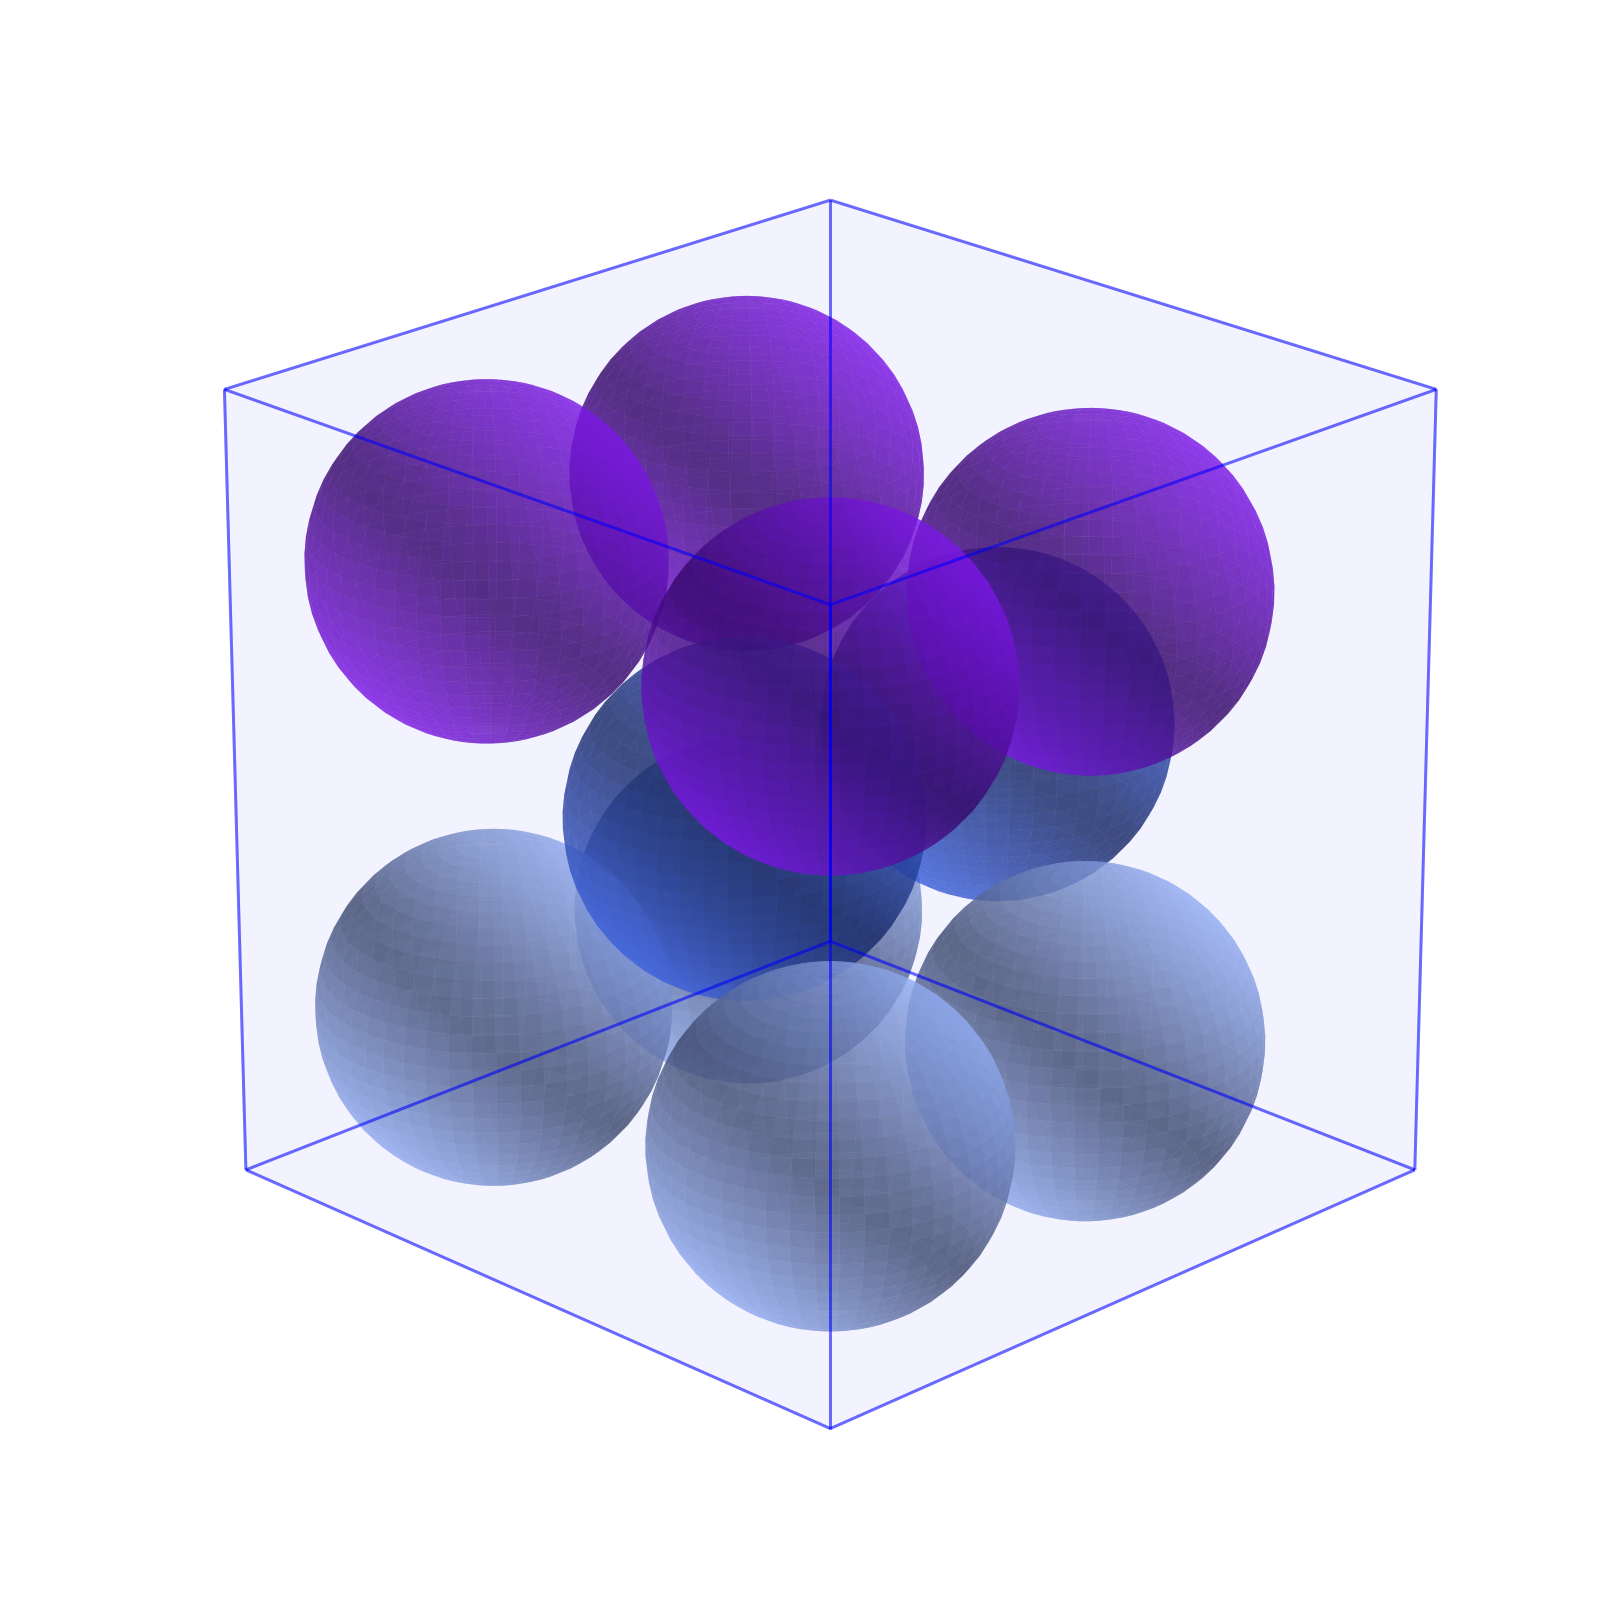
\includegraphics[width=0.3\textwidth]{figures/cube_10.png}
  \caption{Best-achieved 10-point configuration for the
    $p$-dispersion problem in the unit cube using the Euclidean metric
  ($D = \tbd{0.21428571}$).}
  \label{fig:cube_10}
\end{figure}

\begin{figure}[h!]
  \centering
  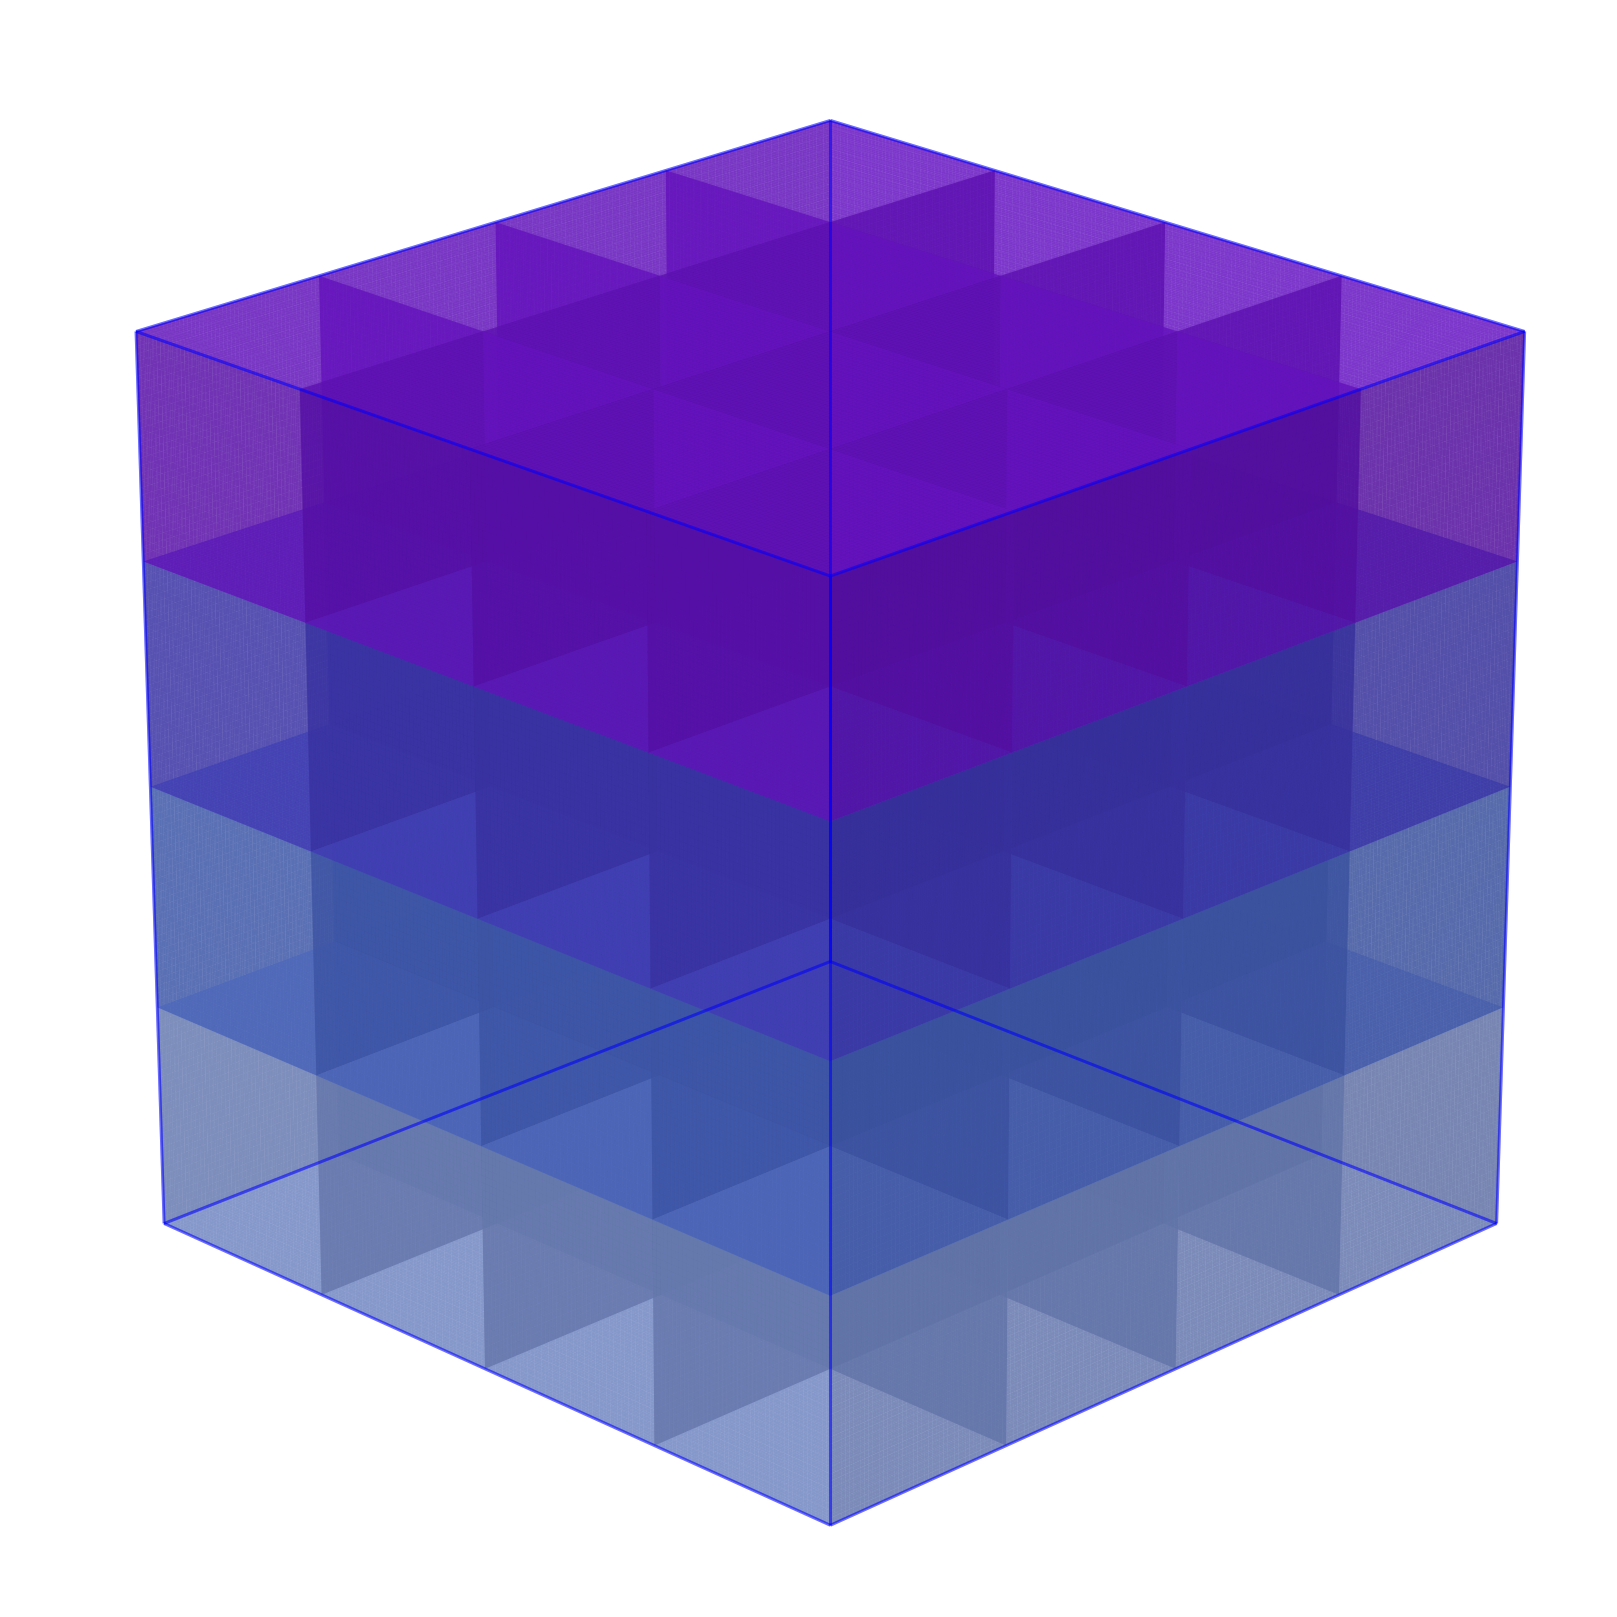
\includegraphics[width=0.3\textwidth]{figures/cube_sup_64.png}
  \caption{Best configuration of $p = 64$ points in the unit cube under the
    $\ell_\infty$ metric ($D = \tbd{0.12499999}$). The optimum is
    $D = \tfrac18$: 64 cubes of side $\tfrac14$ in a $4 \times 4 \times 4$
    grid. Color gives height.}
  \label{fig:cube_sup_64}
\end{figure}

\begin{rvdraft}
Fig.~\ref{fig:cube_10} shows the best Euclidean configuration for ten
points. Under the $\ell_\infty$ metric each ball is an axis-aligned cube of
side $2D$, and at $p = k^3$ the unit cube admits an exact tiling: $k^3$ cubes
of side $\tfrac1k$ fill it, so $D = \tfrac1{2k}$ meets the upper bound of
Lemma~\ref{lem:bracket}, $(V/(\kappa_\infty p))^{1/3} = (1/(8k^3))^{1/3} =
\tfrac1{2k}$, and is optimal. \tbdtext{whether our best radius reaches
the $3 \times 3 \times 3$ grid, $\tfrac16$, at $p = 27$ and the
$4 \times 4 \times 4$ grid, $\tfrac18$, at $p = 64$}
(Fig.~\ref{fig:cube_sup_64}).
\end{rvdraft}

\begin{figure}[h!]
  \centering
  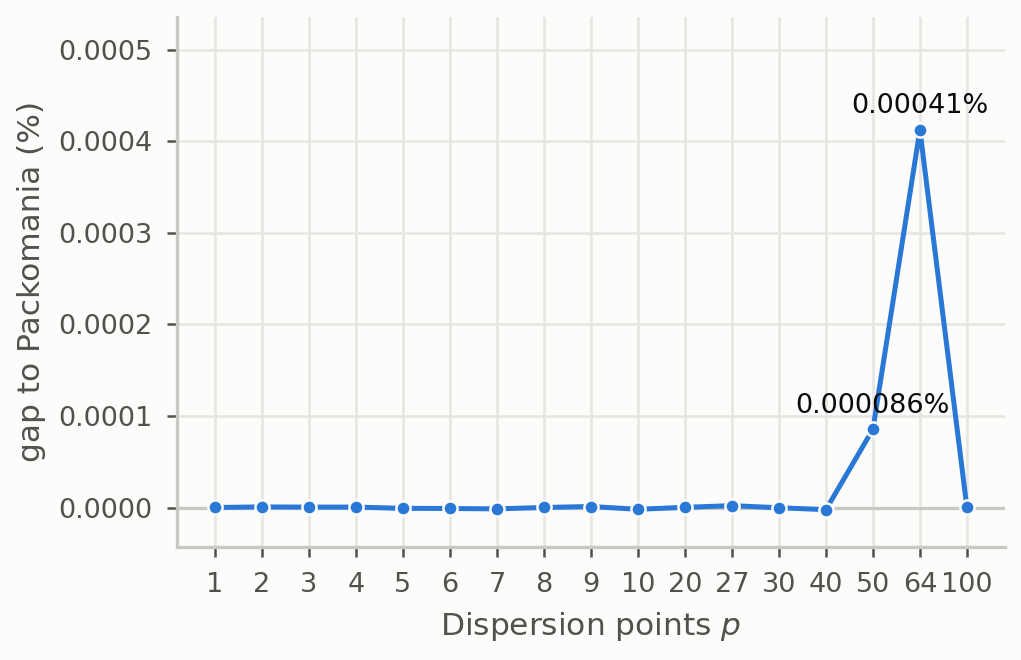
\includegraphics[width=\columnwidth]{figures/comparison_cube.png}
  \caption{Unit cube, Euclidean metric: gap between the Packomania record
    $D_{\mathrm{P}}$ and our best radius $D$, $(D_{\mathrm{P}} - D)/D_{\mathrm{P}}$
    in percent. Zero means our radius matches the record.
    \tbdtext{which $p$ show a gap, and how large}}
  \label{fig:cube_comparison}
\end{figure}

\subsection{Tetrahedron}

\begin{rvdraft}
We benchmark our algorithm against the best-known results for
$p$-dispersion in the unit tetrahedron reported by
\citet{kazakov2018} for $p = 1, \dots, 10$. Additionally, we report
on our best-achieved minimum distances for $p = 20, 35, 56, 84$, the
subsequent tetrahedral numbers. \citet{kazakov2018} mention that for
three-dimensional space, the computational complexity of their
algorithm increases significantly; hence they did not report on
instances for $p > 10$. We use the same settings as for the other
containers. While \citet{kazakov2018} report results up to five
decimal places, we report our results truncated to eight decimal
places to maintain consistency with other sections of this paper.
\end{rvdraft}

Table~\ref{tab:tetrahedron} presents the absolute difference
$A_{\text{err}} = D_{\mathrm{Ours}} - D_{\mathrm{Benchmark}}$ and the
relative percentage improvement $R_{\text{err}}$ between our solution
and the benchmark. \tbdtext{whether our radius is at or above the
benchmark at every $p$}

\resultstable{results_tetrahedron}{tab:tetrahedron}{Tetrahedron: best radius
found in each metric, truncated to eight decimals, with the values of
\citet{kazakov2018} for $\ell_2$. At $p = 1$ the exact answer is the
inradius of the unit regular tetrahedron, $1/(2 \sqrt{6}) = 0.20412415$,
which the benchmark misses by $1.8\%$.}

\begin{figure}[h!]
  \centering
  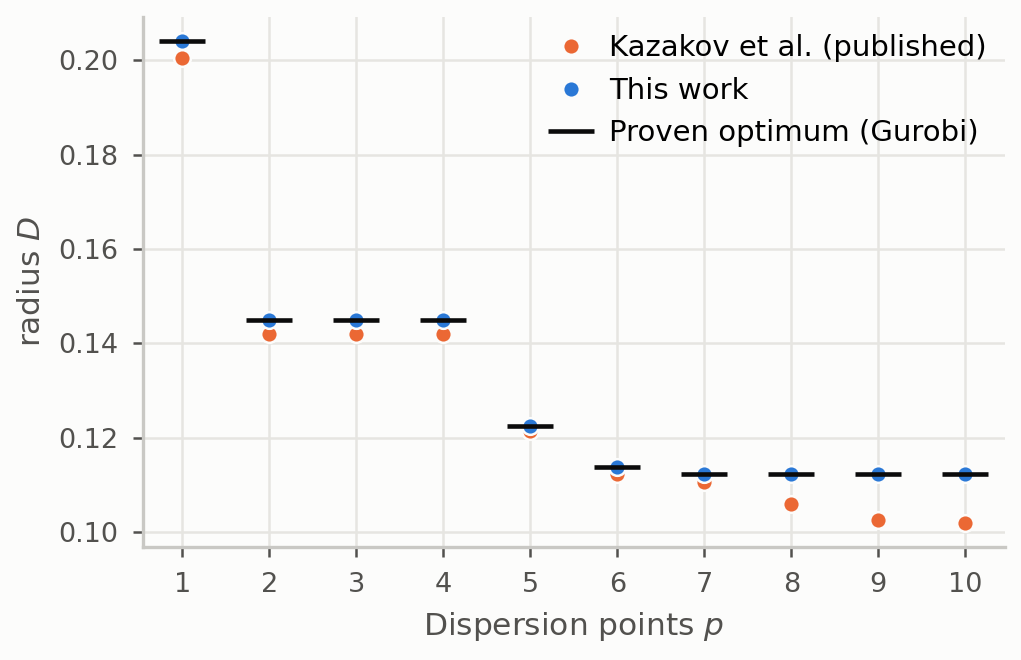
\includegraphics[width=\columnwidth]{figures/comparison_tetrahedron.png}
  \caption{Unit tetrahedron, Euclidean metric: the radius reported by
    \citet{kazakov2018} (orange), our best radius (blue), and the optimum
    Gurobi proves (black dash). The benchmark falls below the optimum by
    $0.8\%$ to $9.2\%$. \tbdtext{whether our radius sits on the proven
    optimum at every $p$}}
  \label{fig:tetra_gap}
\end{figure}

\begin{rvdraft}
To further analyze these improvements, Fig.~\ref{fig:tetra_gap}
illustrates the comparison between our algorithm and the results of
\citet{kazakov2018}: our radius is at or above the published benchmark at every
$p$ it reports \tbdcheck. Gurobi proves that the optimum at $p = 10$ is
$0.112372$ (Section~\ref{sec:baselines}), which our radius matches
\tbdcheck\ and the benchmark misses by $9.2\%$.
\end{rvdraft}

The size of the margin over \citet{kazakov2018} needs a caveat. At $p = 1$
the answer is exactly the inradius of the unit regular tetrahedron,
$1/(2\sqrt{6}) \approx 0.20412$, which we recover to eight decimal places
and the published benchmark misses by $1.8\%$. Since the benchmark is
already $1.8\%$ short where the optimum is elementary, part of our margin
over it reflects the benchmark's limited accuracy rather than the strength
of our algorithm.
Fig.~\ref{fig:tetra_10} provides a visual comparison of the best
configuration found by our algorithm against the corresponding
configuration derived from the parameters in \citet{kazakov2018} for
$p=10$, a tetrahedral number, where the points settle into three
triangular layers of 1, 3 and 6 points.

\begin{figure}[h!]
  \centering
  \begin{subfigure}[b]{\columnwidth}
    \centering
    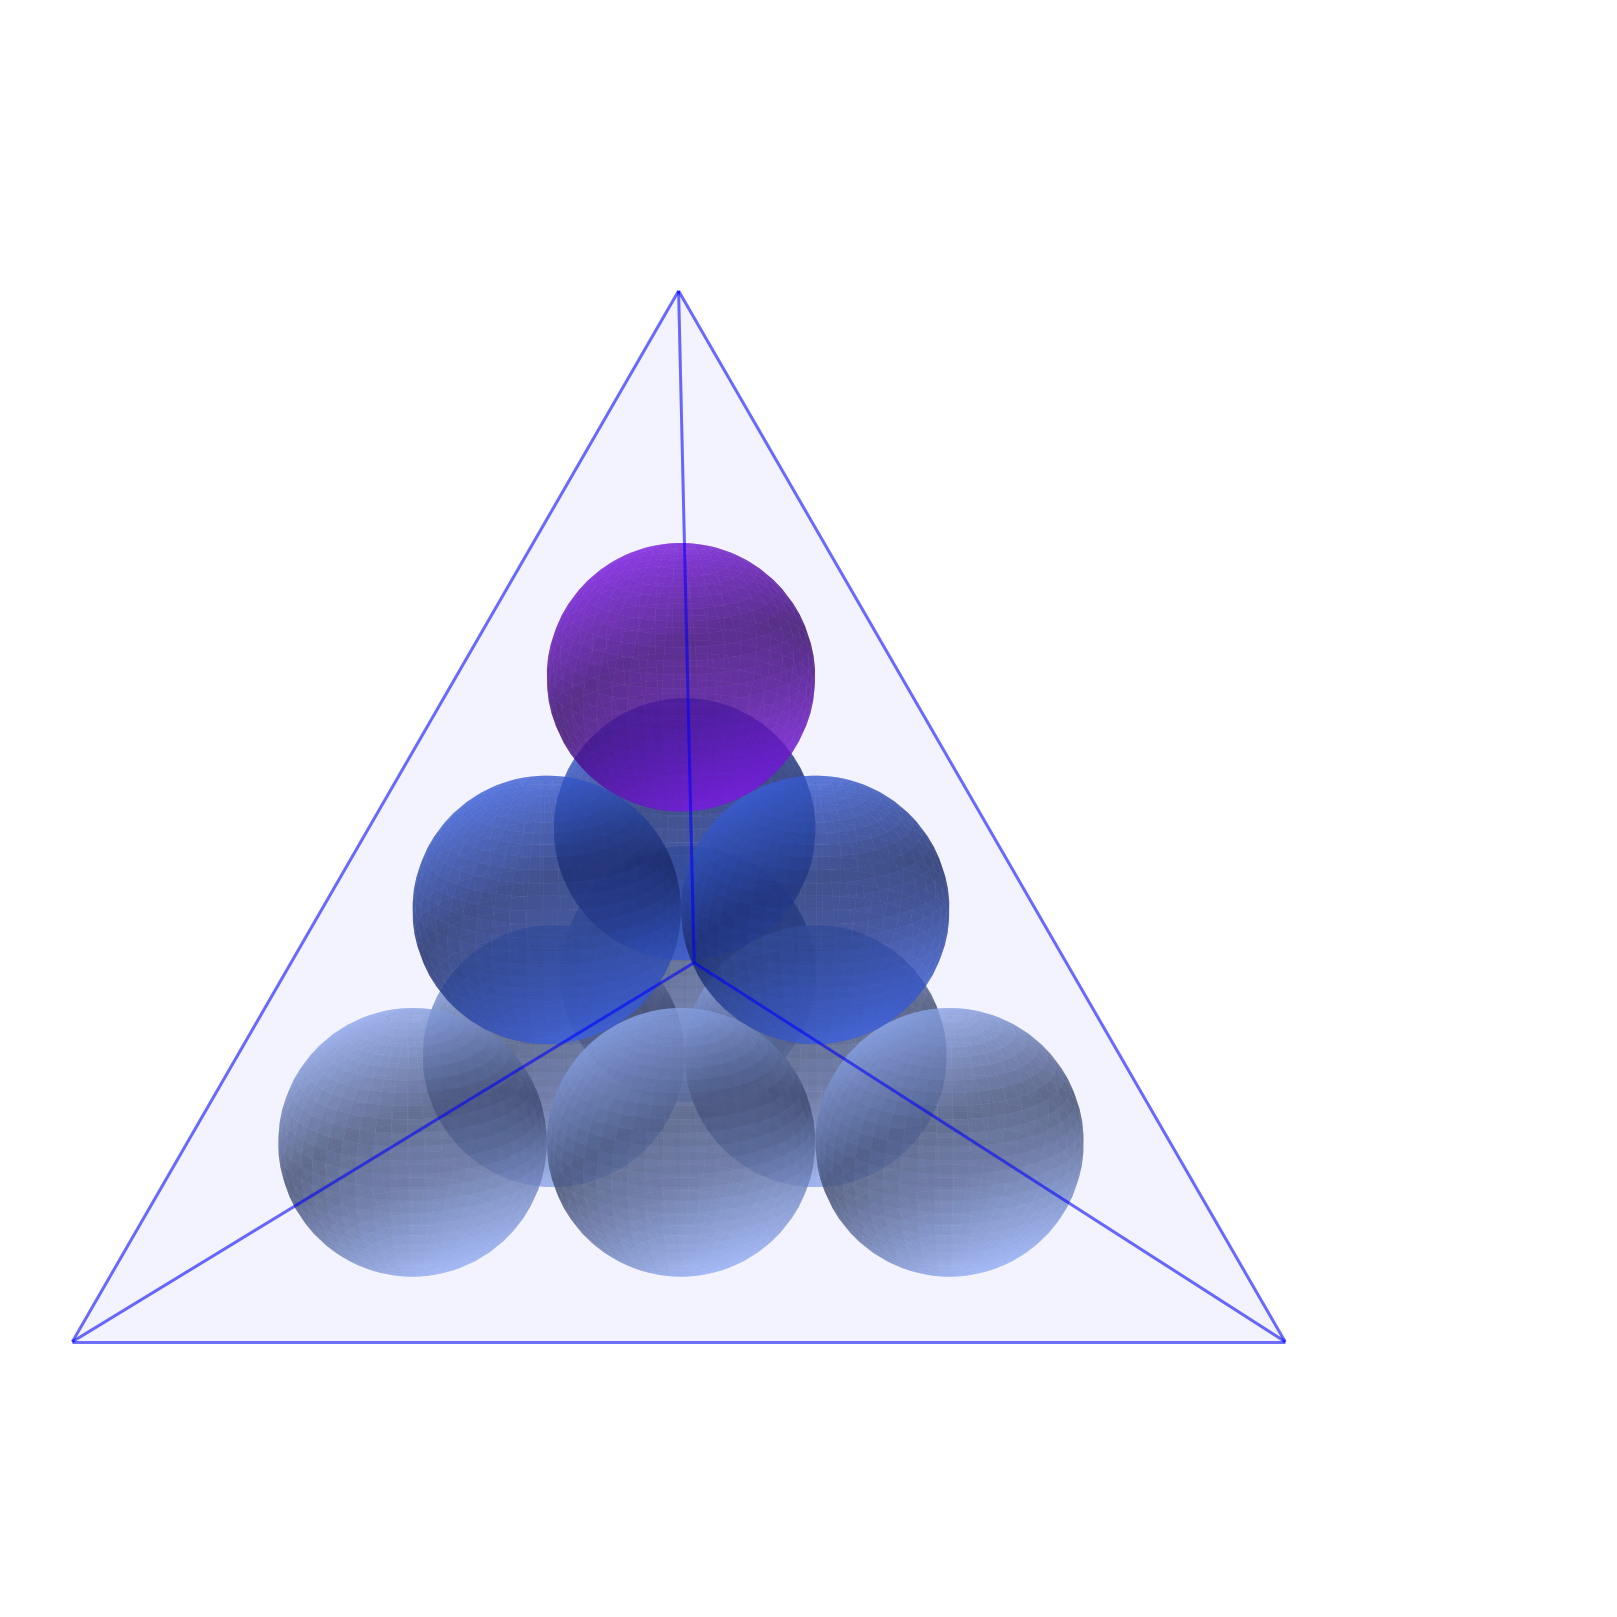
\includegraphics[width=0.7\columnwidth]{figures/tetra_10.png}
    \caption{Our best-achieved configuration for $p=10$ ($D = 0.11237243$).}
    \label{fig:tetra_10_ours}
  \end{subfigure}
  \hfill
  \begin{subfigure}[b]{\columnwidth}
    \centering
    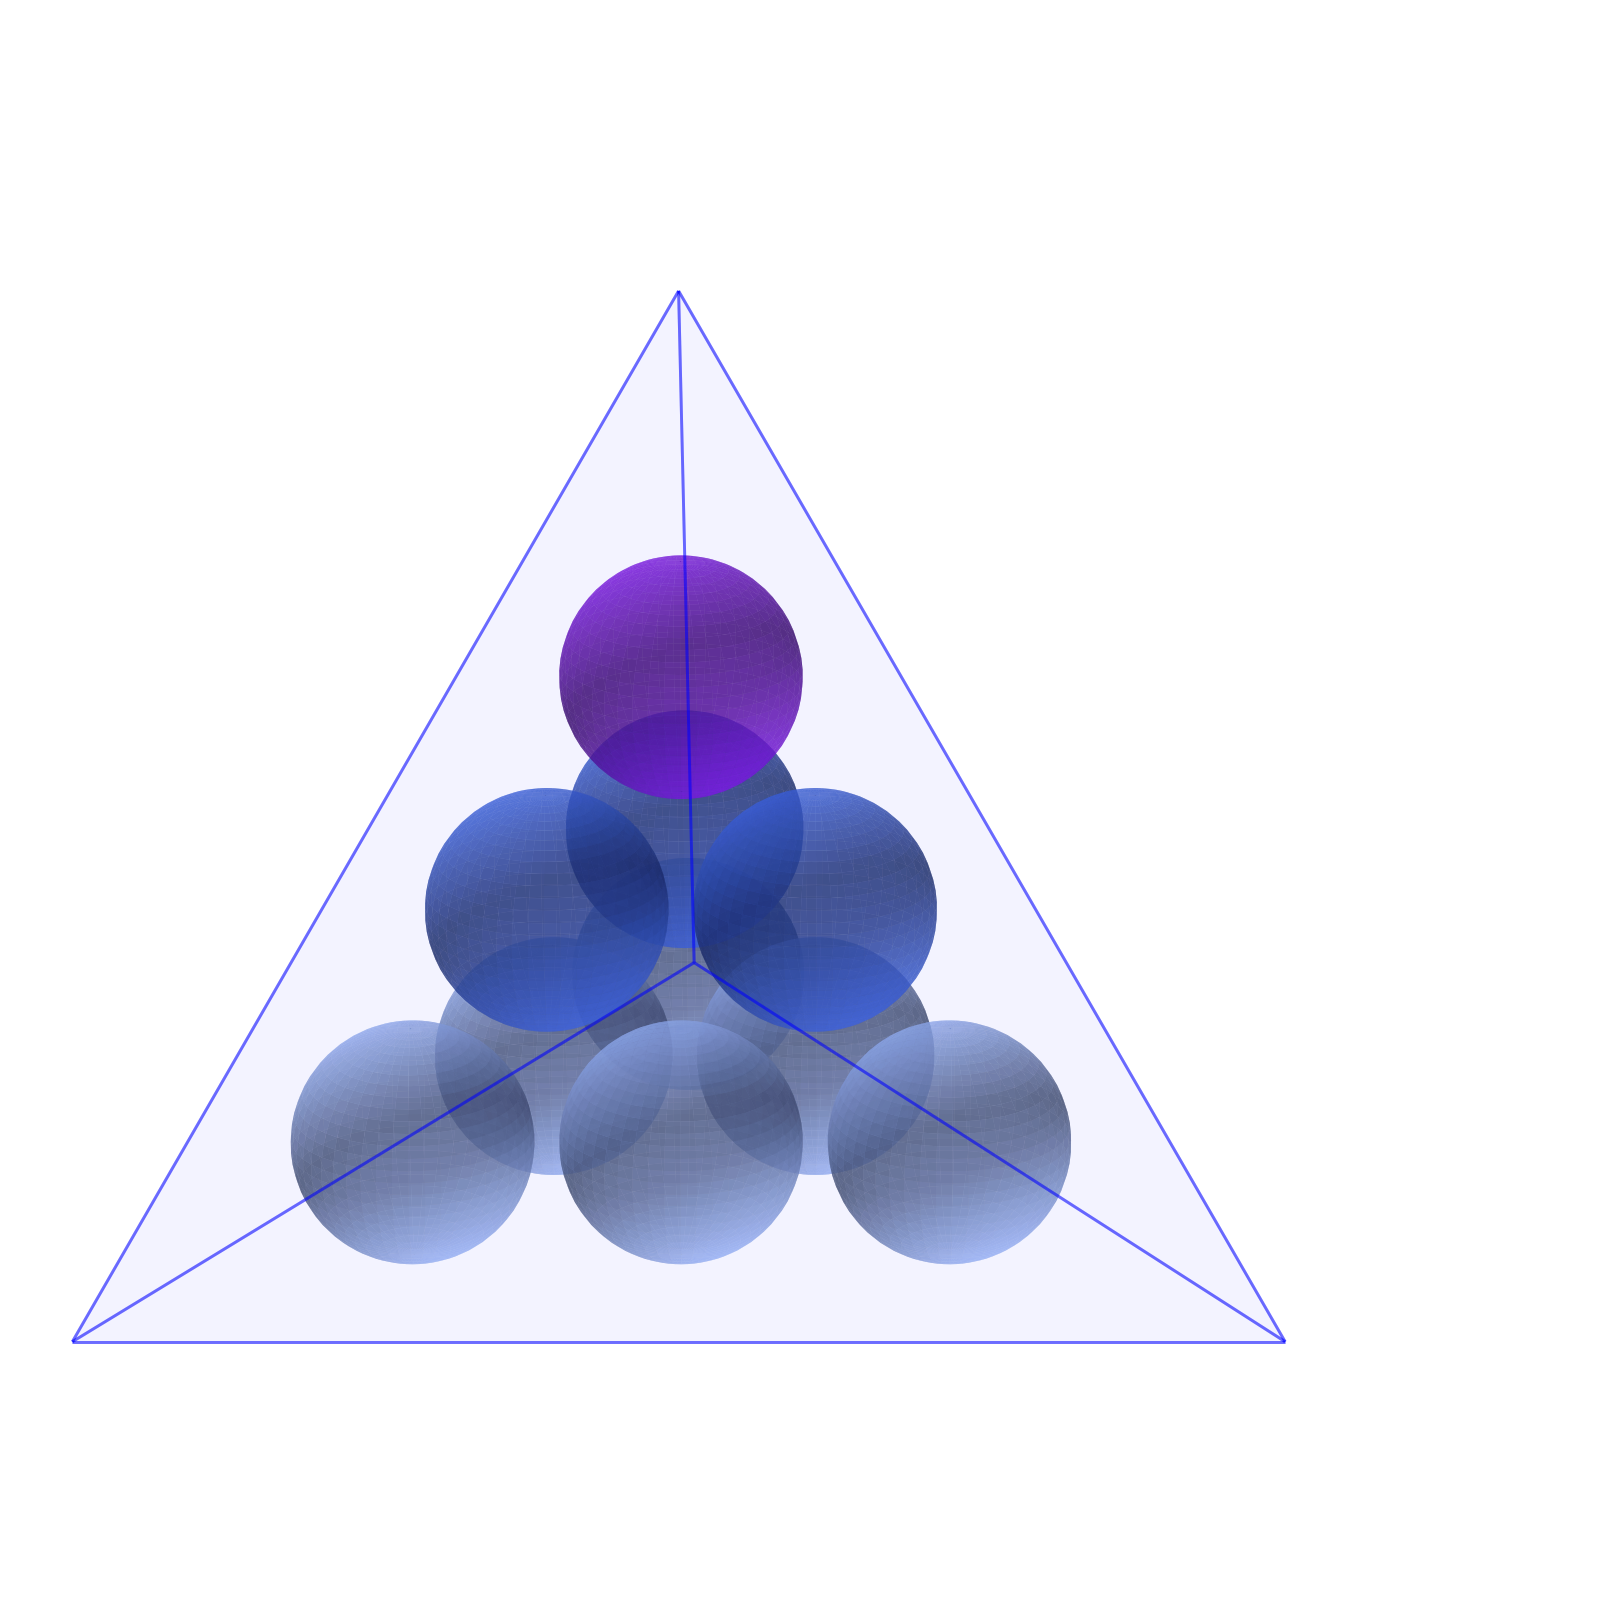
\includegraphics[width=0.7\columnwidth]{figures/kazakov_same_radius_10.png}
    \caption{The same configuration drawn at the radius ($D =
    0.10200$) reported for $p=10$ by \citet{kazakov2018}.}
    \label{fig:tetra_10_kazakov}
  \end{subfigure}
  \caption{Visual comparison of packing density for 10 dispersion
    points in the unit tetrahedron, an improvement of $10.2\%$ over the
    benchmark radius. Both panels show the same configuration from the
    same viewpoint and at the same scale, so the radius is the only
    difference between them: our method (a) leaves the balls in
  contact, while at the benchmark radius (b) visible slack remains.}
  \label{fig:tetra_10}
\end{figure}

Our radius is at least \tbd{0.8}\% larger than that of
\citet{kazakov2018} at every $p$ they report, and the gap grows to
\tbd{10}\% at $p = 10$.

\begin{rvdraft}
Under the other two metrics the balls change shape: under $\ell_1$ each is an
octahedron, under $\ell_\infty$ an axis-aligned cube. Fig.~\ref{fig:tetra_35}
shows the best configurations found for $p = 35$, a tetrahedral number, under
all three metrics.
\end{rvdraft}

Under $\ell_2$ the layers form the tetrahedral pile. For
$p = n(n+1)(n+2)/6$ spheres stacked in $n$ layers, with neighbors touching
and the outer spheres touching the walls, the centers fill a tetrahedron of
edge $2(n-1)D$ inset by $D$ from every face, whose edge is $1 - 2\sqrt6\,D$.
Equating the two gives
\begin{equation}
  D_n = \frac{1}{2\,(n - 1 + \sqrt6)}.
  \label{eq:tetra_pile}
\end{equation}
Our radius matches $D_n$ at every tetrahedral number in our grid,
$p = 4, 10, 20, 35, 56, 84$ ($n = 2, \dots, 7$), to within the relative
$10^{-9}$ by which every reported radius is shrunk \tbdcheck. At
$n = 3$, $D_3 = 1/(2(2 + \sqrt6)) \approx 0.112372$ is the optimum Gurobi
certifies at $p = 10$; for $n \ge 4$ the pile is not known to be optimal, and
we report the match, not optimality.

\begin{figure*}[t]
  \centering
  \begin{subfigure}[b]{0.31\textwidth}
    \centering
    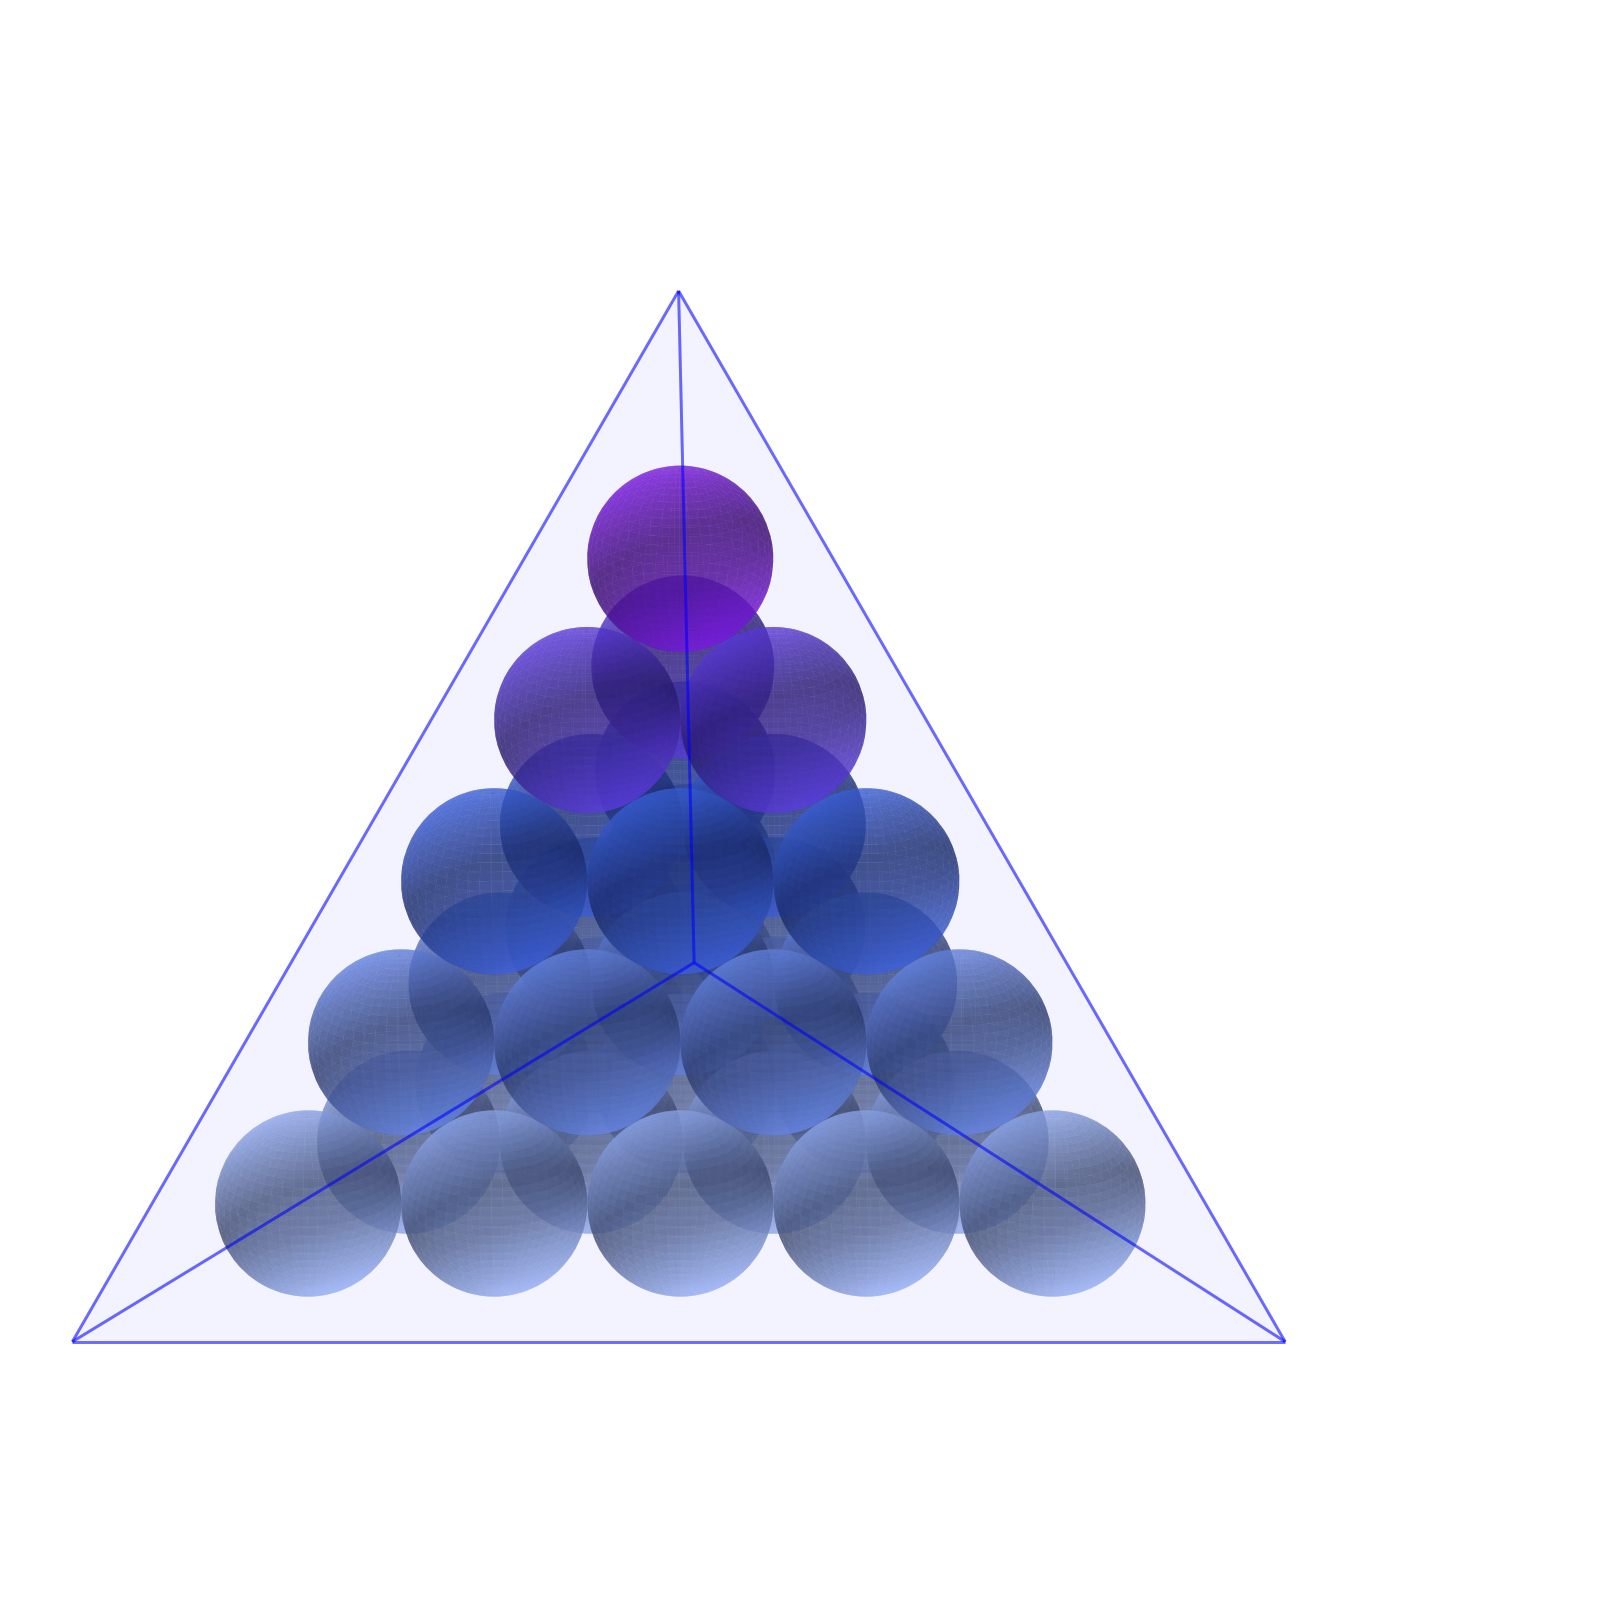
\includegraphics[width=\textwidth]{figures/tetra_l2_35.png}
    \caption{$\ell_2$: spheres ($D = 0.07752551$).}
    \label{fig:tetra_l2_35}
  \end{subfigure}
  \hfill
  \begin{subfigure}[b]{0.31\textwidth}
    \centering
    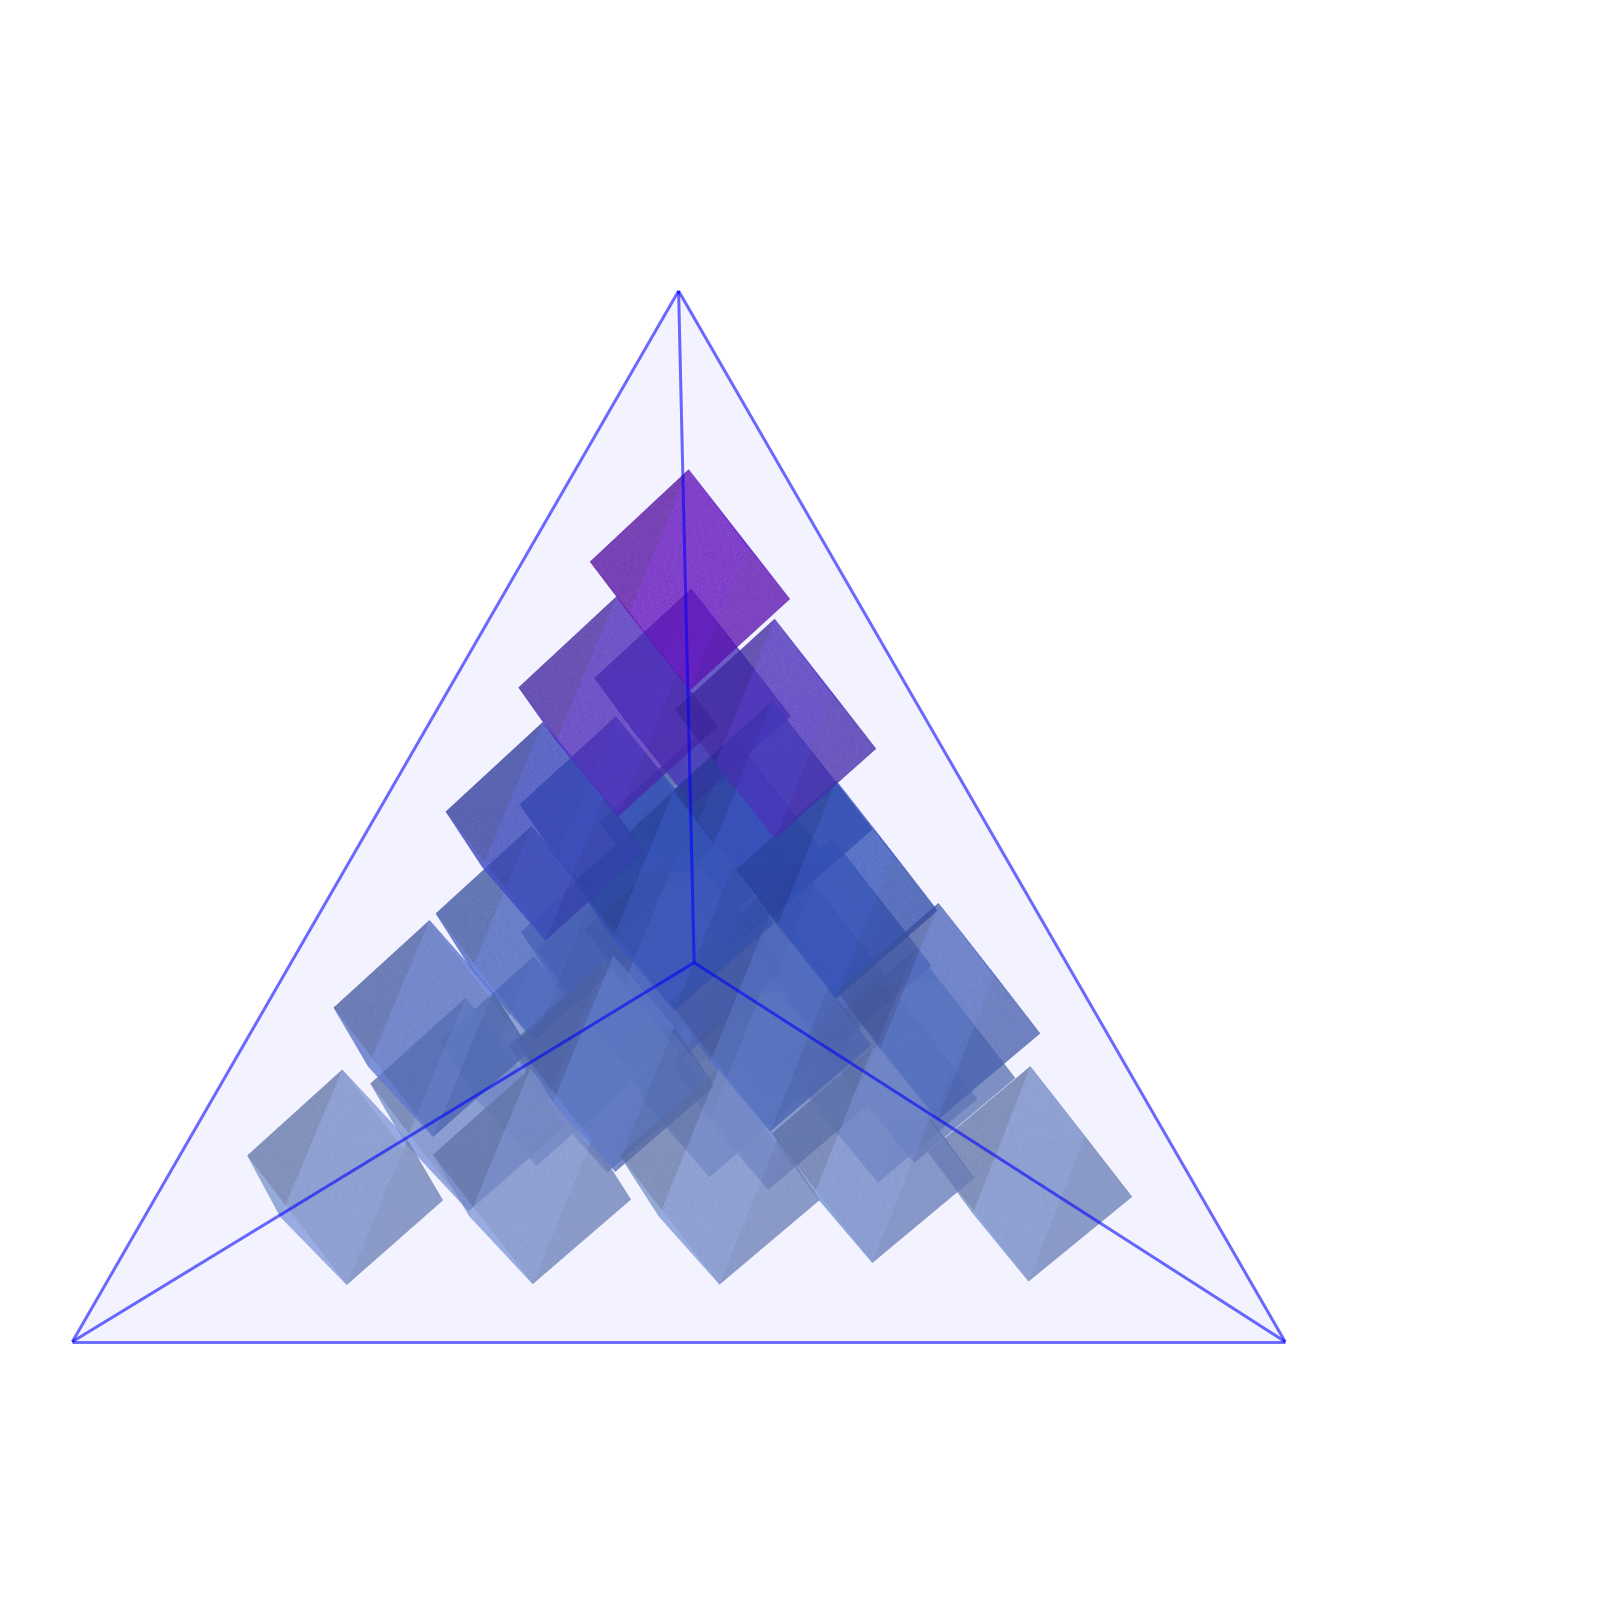
\includegraphics[width=\textwidth]{figures/tetra_l1_35.png}
    \caption{$\ell_1$: octahedra ($D = \tbd{0.09706067}$).}
    \label{fig:tetra_l1_35}
  \end{subfigure}
  \hfill
  \begin{subfigure}[b]{0.31\textwidth}
    \centering
    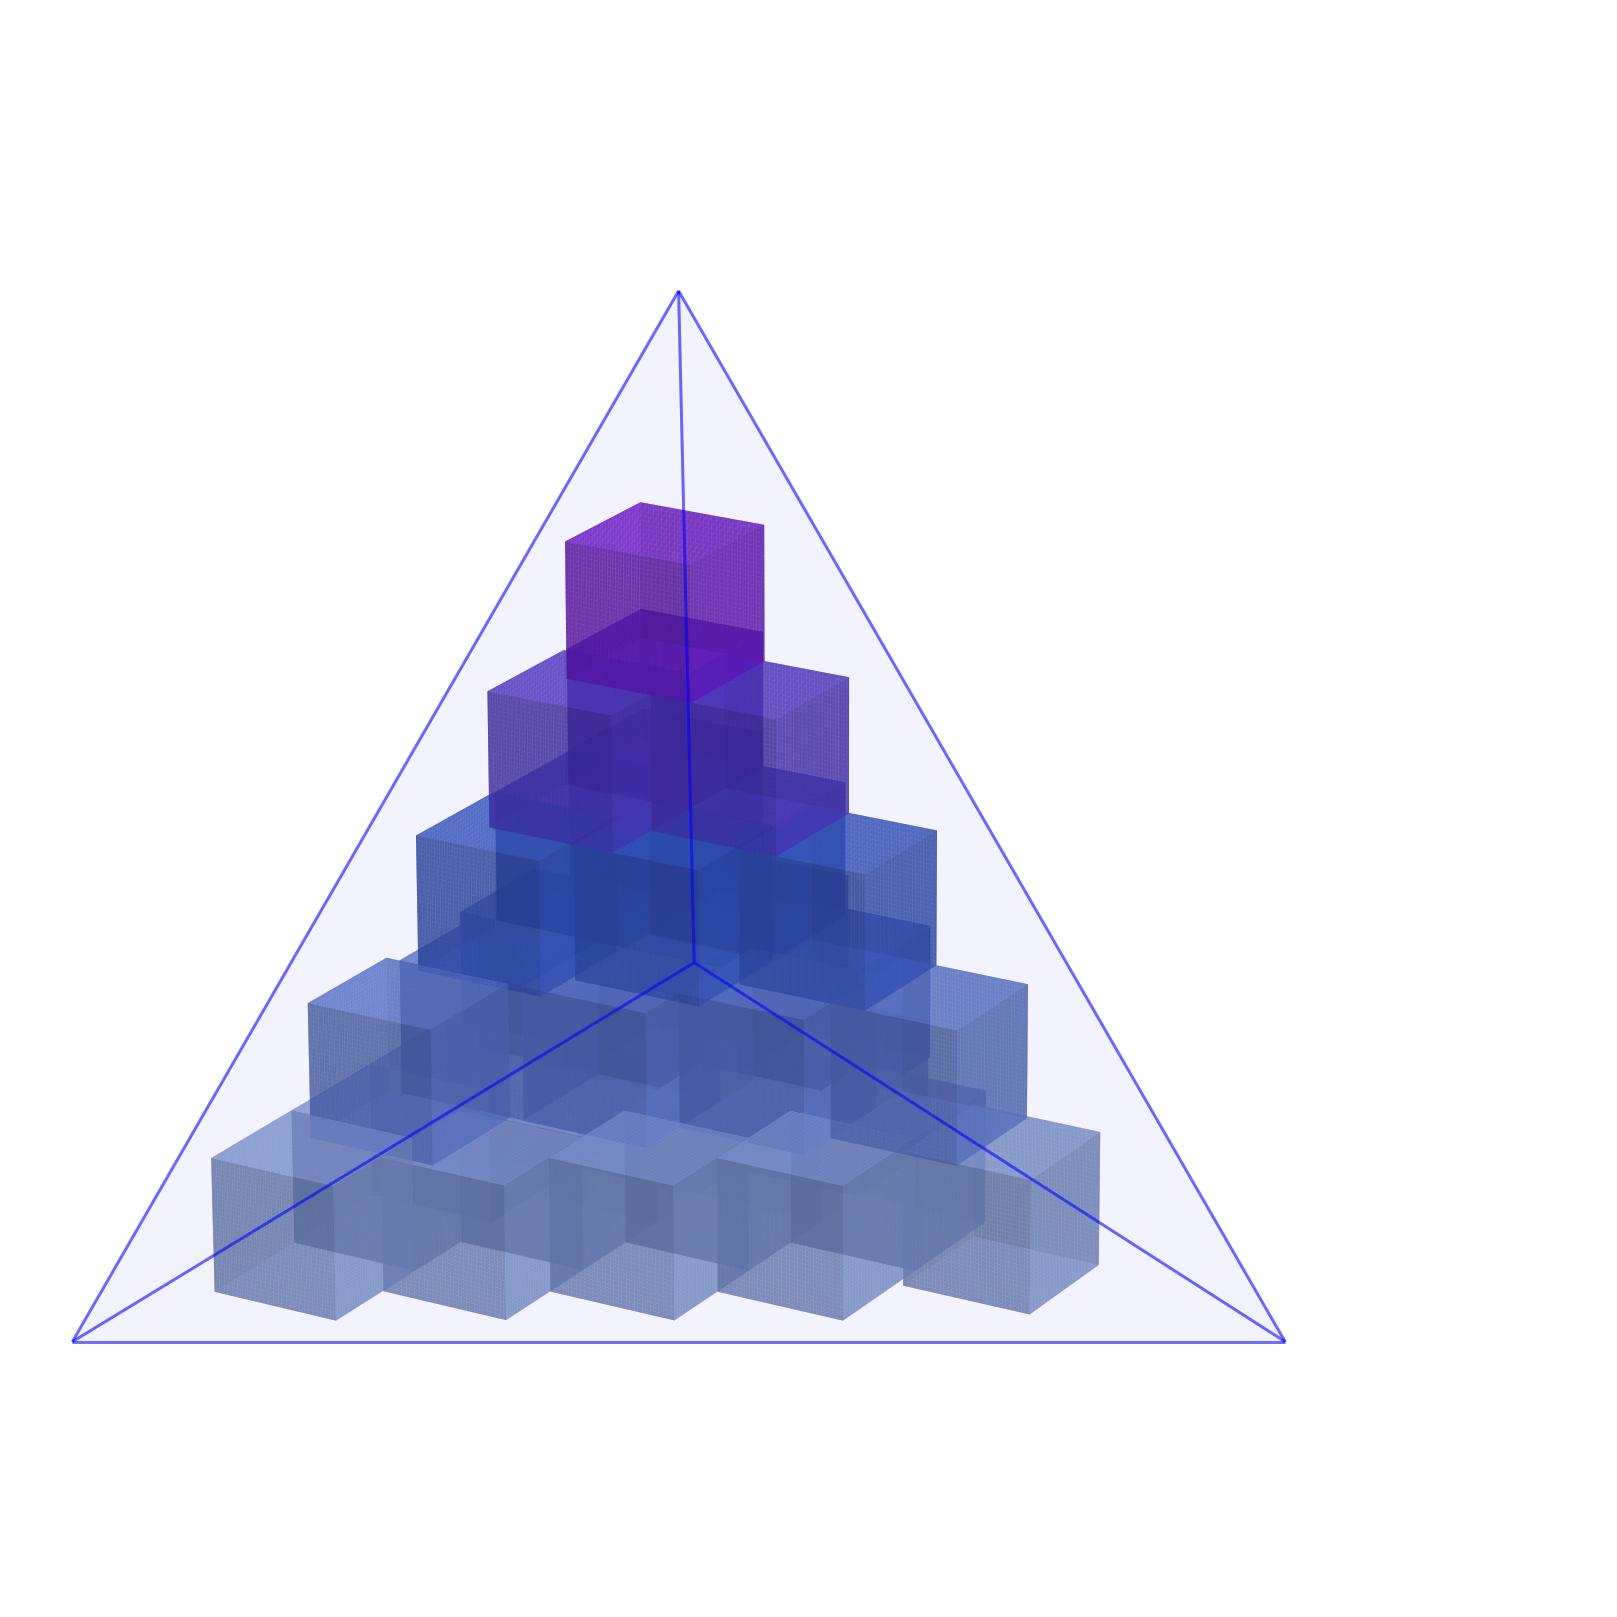
\includegraphics[width=\textwidth]{figures/tetra_linf_35.png}
    \caption{$\ell_\infty$: cubes ($D = \tbd{0.06039796}$).}
    \label{fig:tetra_linf_35}
  \end{subfigure}
  \caption{Best configurations of $p = 35$ points in the unit tetrahedron
    under the $\ell_2$, $\ell_1$ and $\ell_\infty$ metrics. Under $\ell_2$ the
    spheres form the five-layer tetrahedral pile of Eq.~\ref{eq:tetra_pile}.
    Color gives height.}
  \label{fig:tetra_35}
\end{figure*}

\subsection{H-Box}\label{sec:hbox}

Non-convex containers, such as the H-shaped polyhedron, present
significant geometric challenges for the CpDP. Unlike convex domains,
non-convex shapes often feature disconnected feasible regions and
obstructed lines of sight, where the straight-line segment connecting
two valid points may pass through the infeasible exterior
\citep{dai2021}. These characteristics create numerous ``trapped''
local minima that can stall standard optimization algorithms
\citep{lai2024}. The H-shaped polyhedron was created with inspiration
from its two-dimensional analogue: the H-shaped polygon \citep{dai2021}.

Table~\ref{tab:h_box} reports the best radius found for each $p$
in all three metrics. No published values exist for this container; the
comparison with general-purpose solvers is in Section~\ref{sec:baselines}, where
the H-box is one of the containers on which they fall behind.

\resultstable{results_h_box}{tab:h_box}{H-box: best radius found in each
metric, truncated to eight decimals. No published values exist for this
container.}

\begin{rvdraft}
Under the sup norm each ball is an axis-aligned cube of side $2D$, and at
$p = 56$ the H-box admits an exact tiling: 56 cubes of side $\tfrac12$ have total
volume $56 \cdot \tfrac18 = 7$, the volume of the container. The radius
$D = \tfrac14$ therefore meets the upper bound of Lemma~\ref{lem:bracket},
$(V / (\kappa_\infty p))^{1/3} = (7 / (8 \cdot 56))^{1/3} = \tfrac14$, and is
optimal. The tiling needs every cube on the grid at once. Basin hopping,
which accepts only hops that do not raise the residual, cannot build it by
moving a few points, and a restart that is already feasible at a smaller
radius is left unmoved by Tabu Search. Without the escape step, none of 60
runs found the tiling: 24 ended at $D = \tfrac3{14}$ and 36 at
$D = \tfrac16$, $86\%$ and $67\%$ of the optimum. With it, \tbd{20} of 20
runs reach $\tfrac14$, to within the relative $10^{-9}$ by which every
reported radius is shrunk (Fig.~\ref{fig:h_box_sup_56}). Since $p = 56$ is
not in the grid of Table~\ref{tab:h_box}, we ran this cell separately, with
the same settings and 20 seeds.
\end{rvdraft}

\begin{figure}[h!]
  \centering
  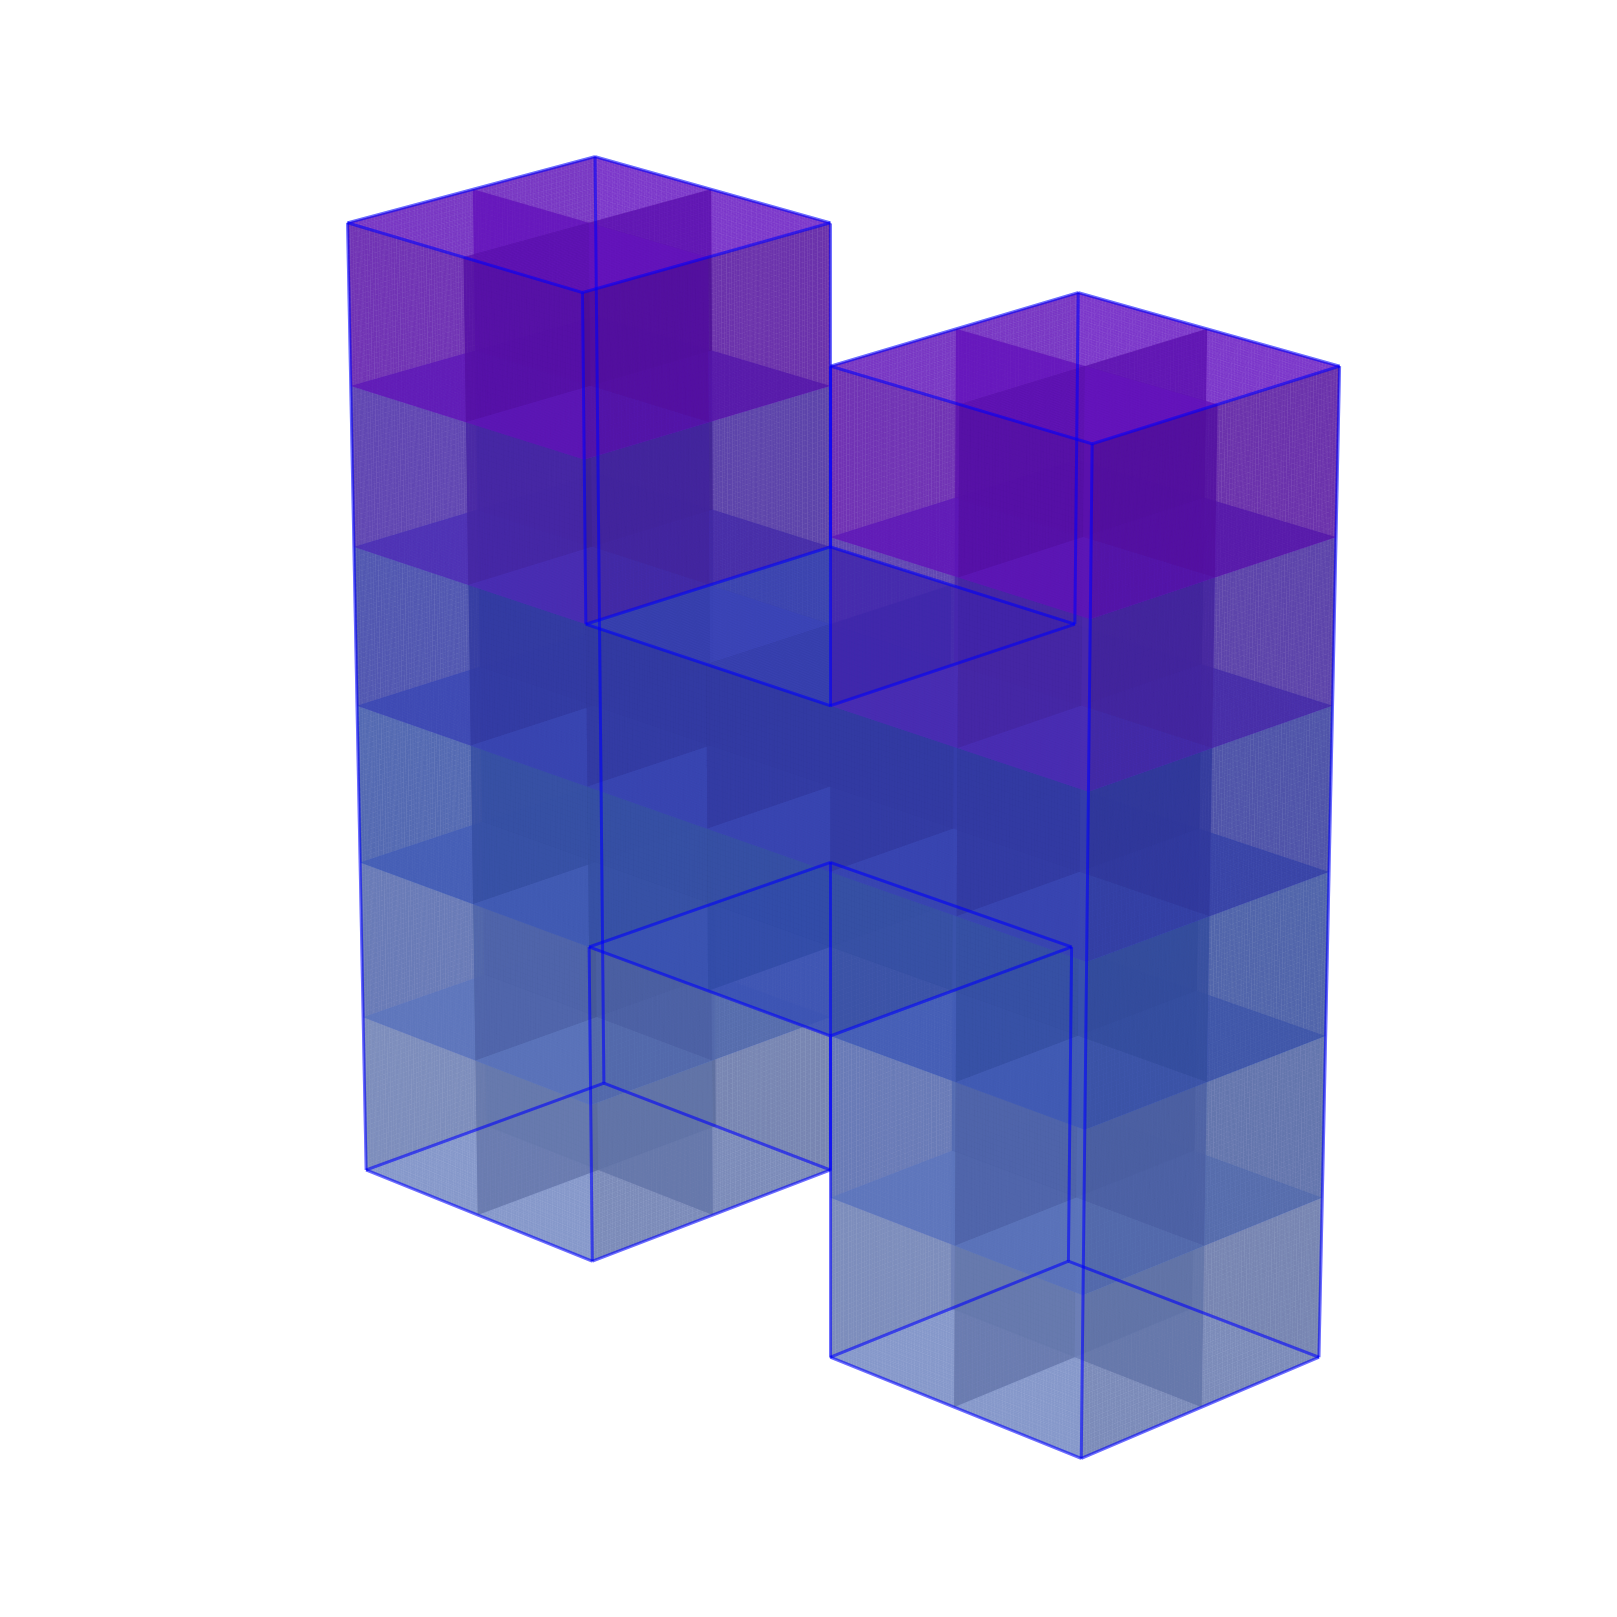
\includegraphics[width=0.35\textwidth]{figures/h-box_sup_56.png}
  \caption{The optimal configuration of $p = 56$ points in the H-shaped
  container under the $\ell_\infty$ metric, $D = \tfrac14$ ($0.24999999$): 56
  cubes of side $\tfrac12$ tile the container exactly. Found in \tbd{20}
  of 20 runs with the escape step, and in none of 60 runs without it. Color
  gives height, so each layer of the tiling shows as a band.}
  \label{fig:h_box_sup_56}
\end{figure}

\subsection{Star-Shaped Polyhedron}

The star-shaped polyhedron draws inspiration from the Kepler-Poinsot
polyhedron \citep{coxeter1989} and serves as a rigorous test case for
non-convex optimization due to its distinctive central convex core
connected to six narrow, tapering spikes. This originally developed
geometry creates significant ``bottlenecks'' between the feasible
sub-regions, making it difficult for optimization algorithms to
migrate points from one spike to another. Unlike convex containers
where local descent directions are often globally informative, the
star-shaped polyhedron requires an algorithm capable of traversing
infeasible space to escape the local optima found within individual spikes.

\begin{rvdraft}
In Table~\ref{tab:pointy_star}, we report the best minimum
distances ($D_{\mathrm{Ours}}$) achieved by our algorithm for a range
of $p$ values, up to $p = 100$.
\end{rvdraft}

\resultstable{results_pointy_star}{tab:pointy_star}{Star: best radius found
in each metric, truncated to eight decimals. No published values exist for
this container.}

For $p = 1$ the algorithm places the point in the central core. Up to
$p = 6$ it puts one point in each of the six spikes, keeping the radius at
$D \approx \tbd{0.9030}$. From $p = 7$ on, the core and the spikes fill up
and the radius decreases gradually.

\begin{rvdraft}
Fig.~\ref{fig:ps_100} shows the best configuration found for $p = 100$.
\tbdtext{how many balls sit in the central core and in each spike, and how
far toward the tips the outermost centers lie}. The algorithm does not crowd
the core and leave the spikes empty: it carries points through the
bottlenecks and fills every spike.
\end{rvdraft}

\begin{figure}[h!]
  \centering
  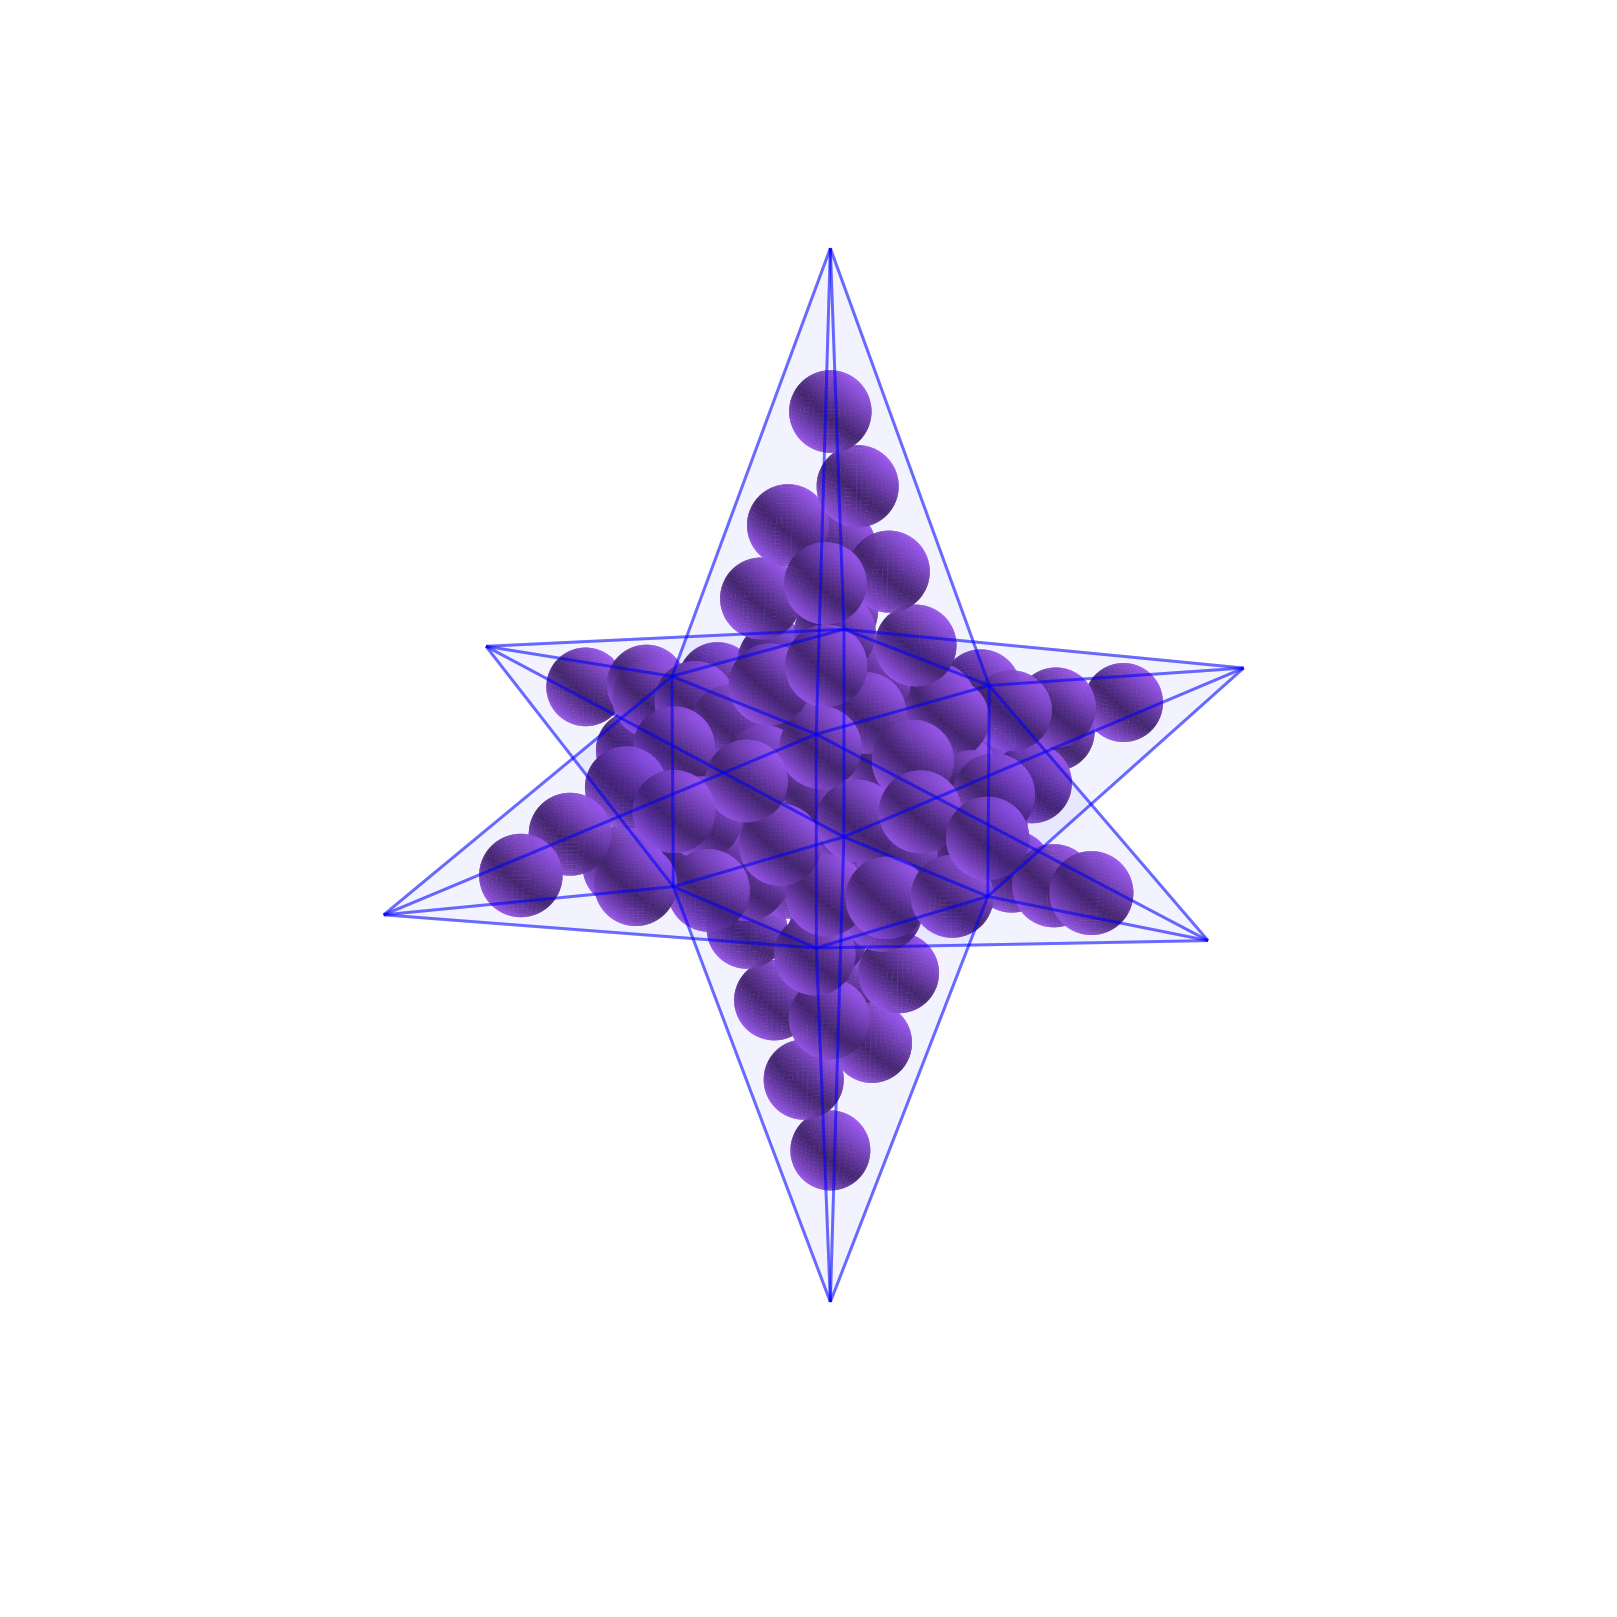
\includegraphics[width=0.85\columnwidth]{figures/ps_100.png}
  \caption{Best achieved configuration of $p = 100$ points in the star-shaped
  container under the Euclidean metric ($D = \tbd{0.36219729}$).
  \tbdtext{balls in the core and in each spike}}
  \label{fig:ps_100}
\end{figure}

\subsection{Ribbed Ventilation Cage}

Finally, we apply our algorithm to the ``ribbed ventilation cage,'' a
highly complex non-convex polyhedron designed to model modern
industrial computer casings and heat sinks. Unlike the H-shaped box
or Star-shaped polyhedron, which feature large distinct sub-regions,
this container is characterized by numerous corridors and separated
legs. The inclusion of numerous internal pillars and ribs creates a
``maze-like'' feasible region, introducing frequent discontinuities
that pose severe challenges for traditional gradient-based nonlinear optimizers.

The particular design of this ribbed ventilation cage polyhedral
container is original, although the complexity is practically
motivated. In thermal engineering, components utilize ribbed
structures, fins, and microstructures to maximize surface area and
improve heat dissipation capabilities \citep{xin2025}. Solving the
CpDP on such a geometry is therefore relevant for optimizing the
layout of sensors, cooling pipes, or modular components within
densely packed electronic enclosures. We evaluate our algorithm using
both the Euclidean metric ($\ell_2$), representing standard spherical
component packing, and the sup-norm ($\ell_\infty$), which is
critical for modeling the placement of cubic or box-shaped components
often found in hardware design.

Table~\ref{tab:cage} reports the best radius found for each $p$ in all three
metrics.

\resultstable{results_cage}{tab:cage}{Cage: best radius found in each
metric, truncated to eight decimals. No published values exist for this
container.}

Fig.~\ref{fig:cage_100_l2} and Fig.~\ref{fig:cage_100_sup} show the best
configurations found for $p = 100$ points in this container under the
Euclidean and $\ell_\infty$ metrics.

\begin{rvdraft}
The cage has a trap of its own: without the escape step, many cage runs
stopped at exactly $D = \tfrac12$, among them 16 of 20 at $p = 100$ under
$\ell_2$. \tbdtext{how many cage runs stop at $D = \tfrac12$ with the
escape step, and the effect on the best radius at $p = 100$}
\end{rvdraft}

\begin{figure}[H]
  \centering
  \begin{minipage}[t]{0.4\textwidth}
    \centering
    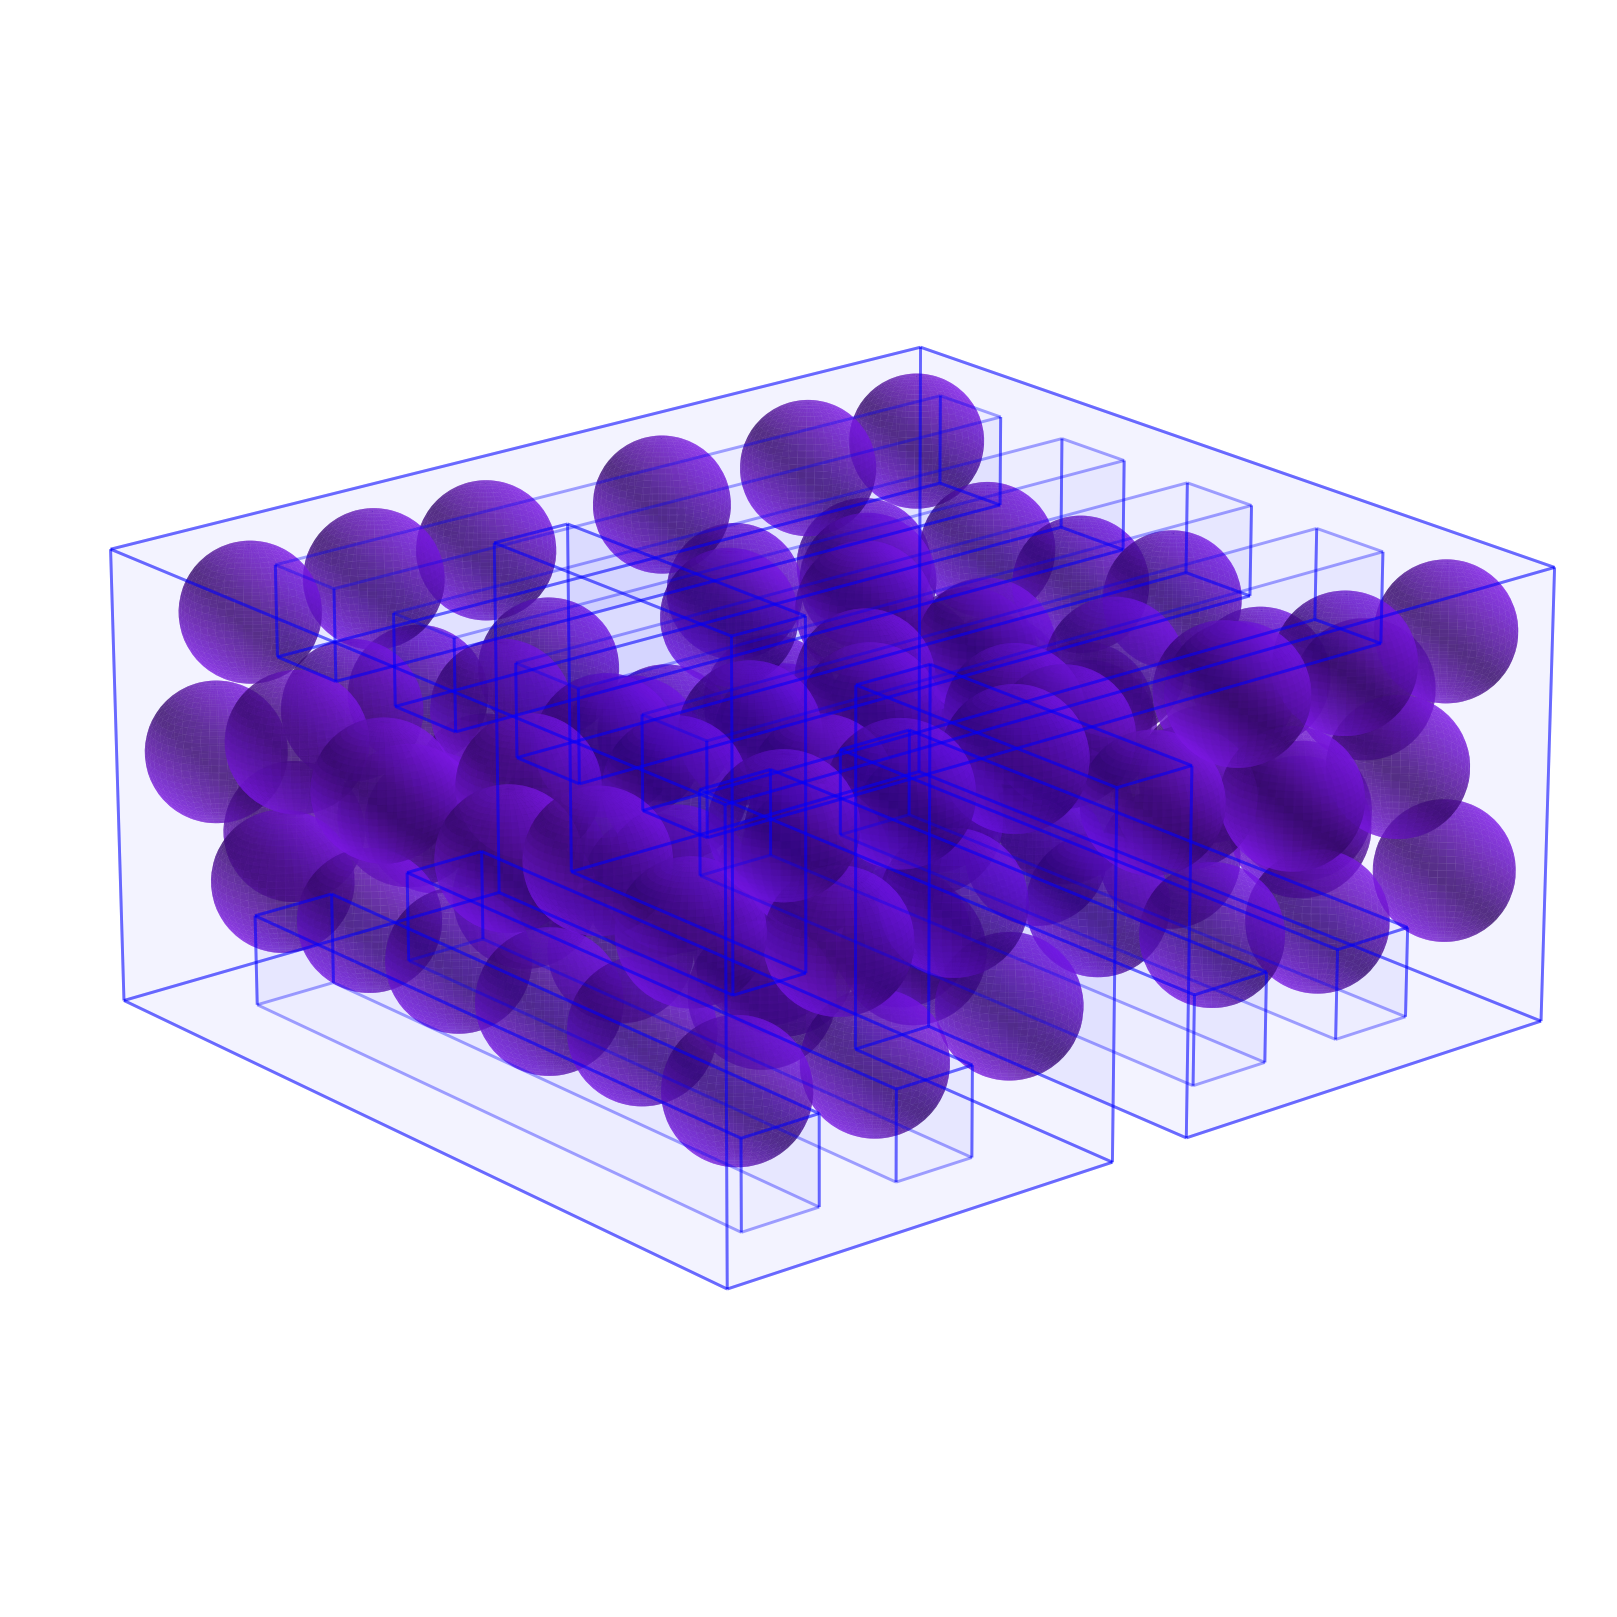
\includegraphics[width=\textwidth]{figures/cage_100.png}
    \caption{Best achieved configuration for $p = 100$ points using
    the Euclidean metric ($D = \tbd{0.74175552}$).}
    \label{fig:cage_100_l2}
  \end{minipage}\hfill
  \begin{minipage}[t]{0.4\textwidth}
    \centering
    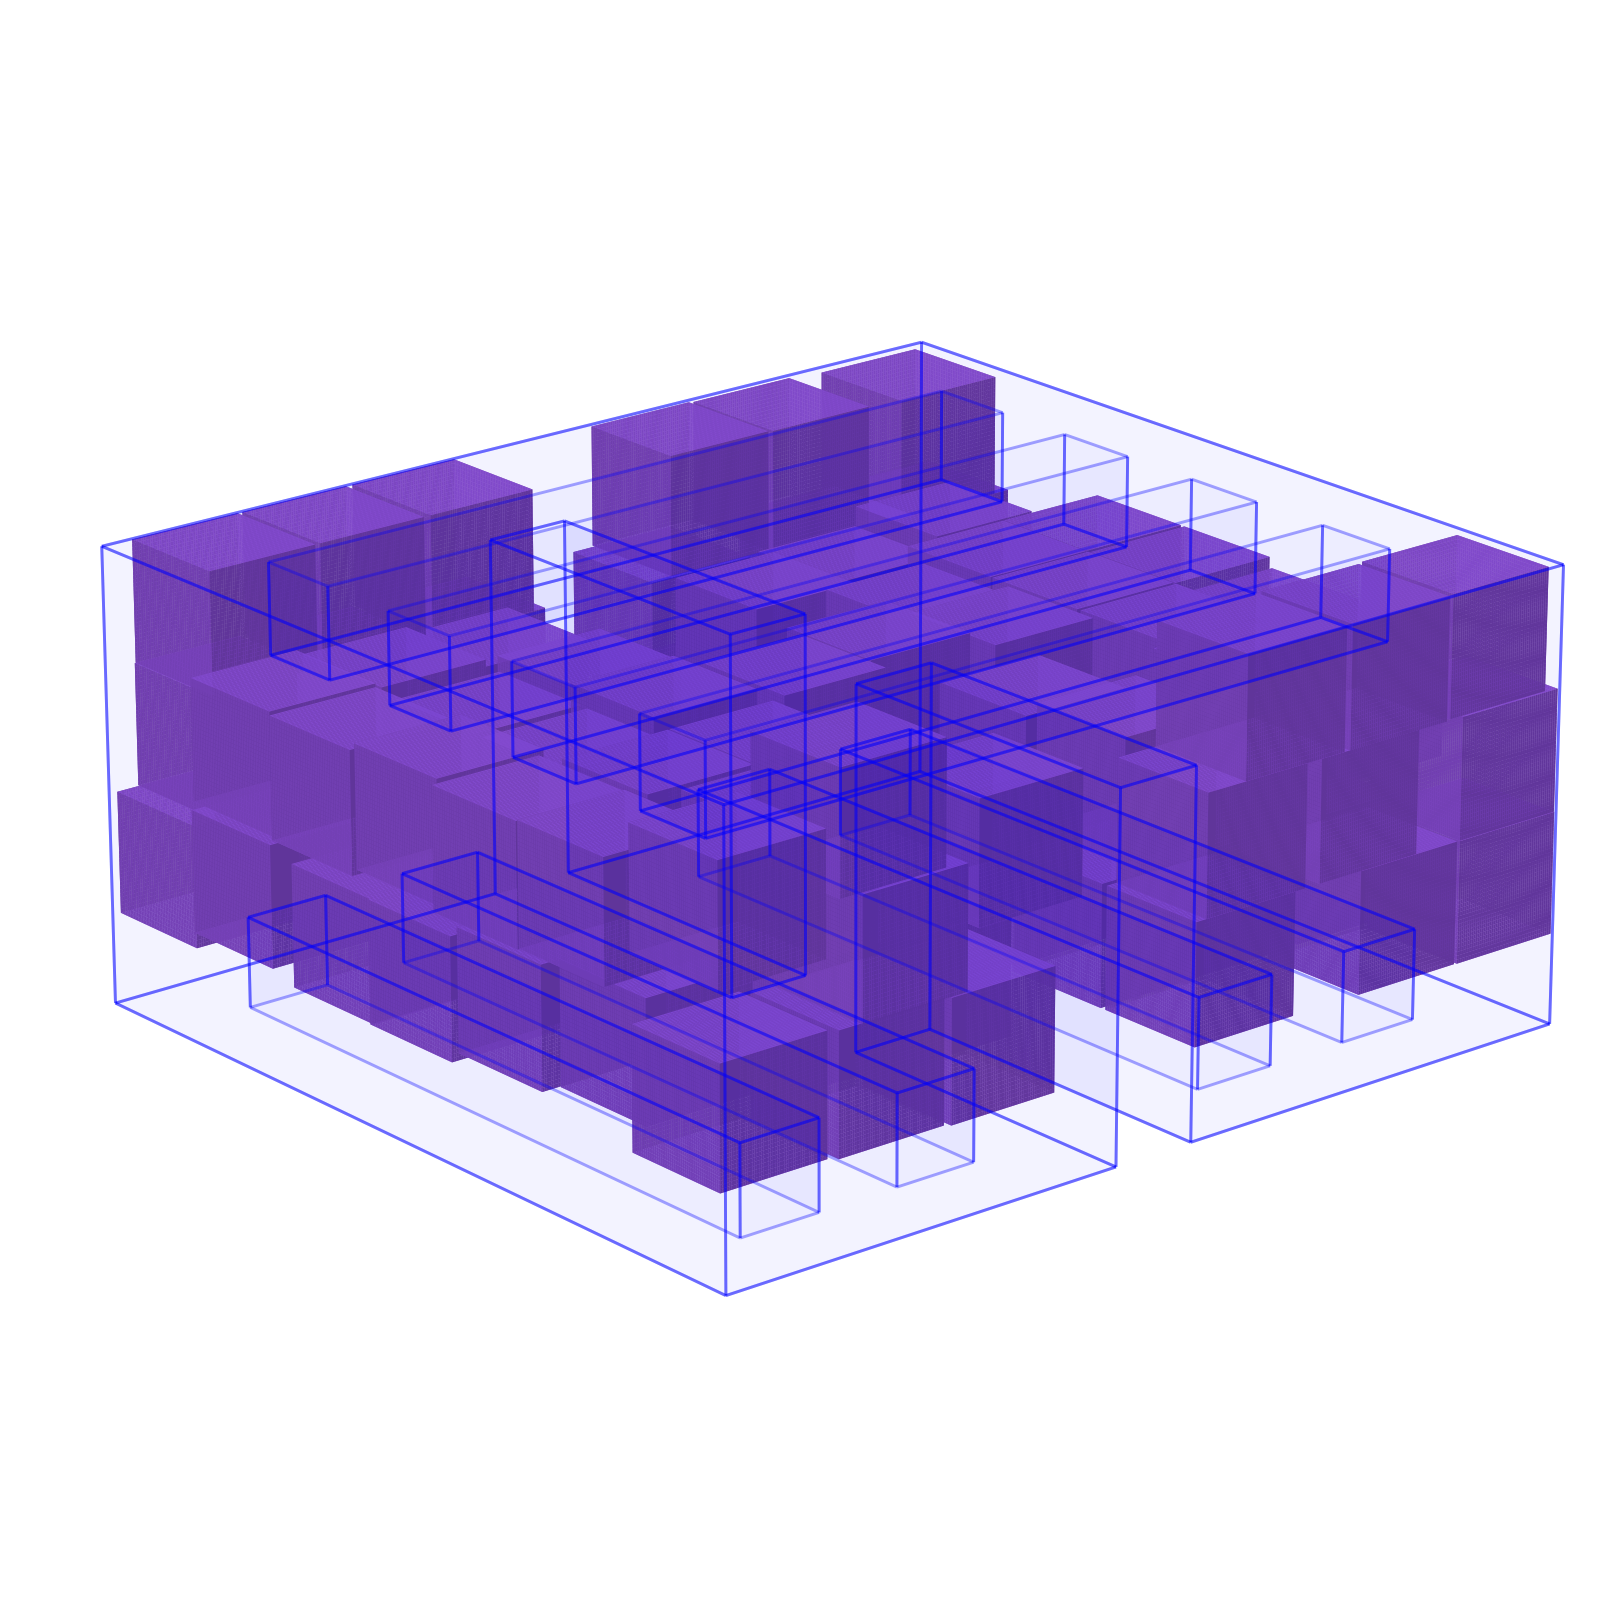
\includegraphics[width=\textwidth]{figures/cage_sup_100.png}
    \caption{Best achieved configuration for $p = 100$ points using the
    $\ell_\infty$ metric ($D = \tbd{0.66666666}$).}
    \label{fig:cage_100_sup}
  \end{minipage}
\end{figure}

At $p = 100$ the points spread through the corridors between the pillars
and ribs rather than collecting in the open regions of the cage.

\subsection{Comparison with Stoyan and Yaskov}\label{sec:stoyan}

\begin{rvdraft}
\citet{stoyan2013} pack congruent spheres of radius one into eight
multi-connected polyhedral domains: a truncated box, or a cuboid, from which
through-prisms, polyhedral cones and dihedral angles are removed, so that the
domain has holes. For each they report the largest number of spheres they
packed and the time it took. Under $\ell_2$, $p$ spheres of radius one fit
exactly when $D^*(p) \ge 1$. We rebuilt the eight domains from the coordinates given
in their paper and ran our algorithm with the settings of the main experiment,
10 seeds per count, at their count and the four counts above it, and further
in the two domains where every one of those counts fitted. A count is fitted
when some seed returns a certified radius of at least one.
\end{rvdraft}

\begin{table}[t]
  \caption{Spheres of radius one packed into the eight domains of
    \citet{stoyan2013}: their count, ours, our best radius at their count,
    and the time at which one of our runs first held radius one at their
    count, against their reported time.}
  \label{tab:stoyan}
  \centering
  \small
  \setlength{\tabcolsep}{4pt}
  \begin{tabular}{ccccrr}
    \hline
    & \multicolumn{2}{c}{Spheres} & & \multicolumn{2}{c}{Time (min)} \\
    Example & Theirs & Ours & $D$ at theirs & Ours & Theirs \\
    \hline
    1 & 93 & \tbd{97} & \tbd{1.0068} & \tbd{6.8} & 41 \\
    2 & 91 & \tbd{93} & \tbd{1.0069} & \tbd{2.3} & 34 \\
    3 & 86 & \tbd{88} & \tbd{1.0069} & \tbd{1.6} & 47 \\
    4 & 81 & \tbd{82} & \tbd{1.0065} & \tbd{1.9} & 54 \\
    5 & 79 & \tbd{79} & \tbd{1.0045} & \tbd{3.5} & 60 \\
    6 & 30 & \tbd{31} & \tbd{1.0072} & \tbd{0.9} & 2 \\
    7 & 58 & \tbd{59} & \tbd{1.0059} & \tbd{0.9} & 7 \\
    8 & 73 & \tbd{80} & \tbd{1.0326} & \tbd{0.2} & 12 \\
    \hline
  \end{tabular}
\end{table}

\begin{rvdraft}
We fit more spheres than published in \tbd{seven} of the eight domains, by
\tbd{one} to \tbd{seven}, and as many in \tbdtext{the rest}
(Table~\ref{tab:stoyan}, Fig.~\ref{fig:stoyan}). At their published counts,
\tbd{71} of our 80 runs reach radius one, and the first does so within
\tbd{7} minutes in every domain. Their
times were measured on an AMD Athlon 64 X2 6000+ in Delphi, \rvdecide{so the time
columns indicate scale rather than a like-for-like comparison.}
Fig.~\ref{fig:stoyan_packings} shows each domain at our count.
\tbdtext{where the gains are largest}
\end{rvdraft}

\begin{figure*}[t]
  \centering
  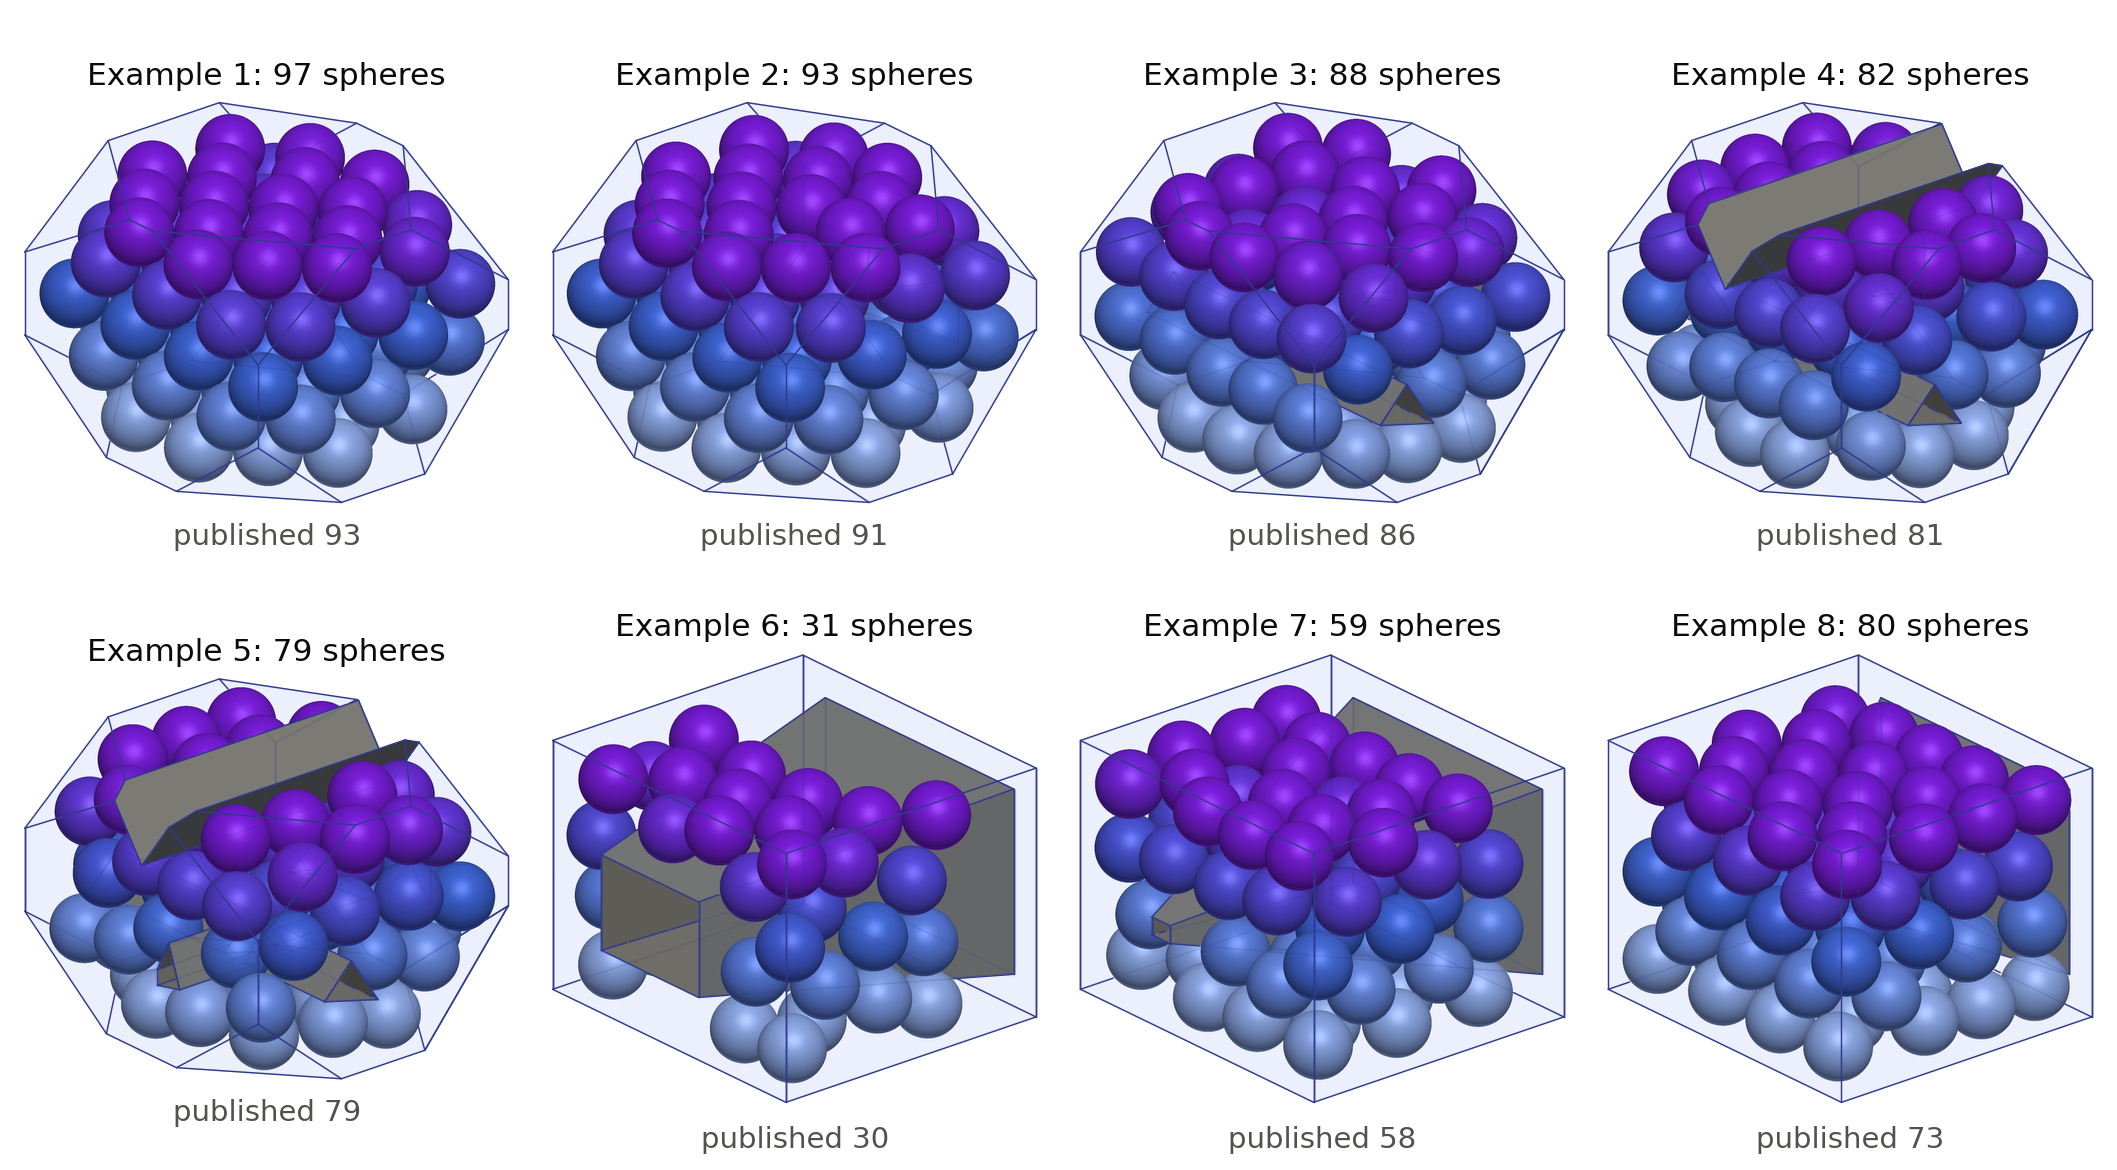
\includegraphics[width=\textwidth]{figures/stoyan_yaskov_packings.png}
  \caption{The most spheres of radius one we fit into each domain of
    \citet{stoyan2013}, best seed of that count; their published count below.
    The removed pieces (prisms, cones, dihedral angles and the tapered holes
    of examples 6 to 8) are drawn in gray, and spheres are shaded by height.
    The centers of these and every other configuration we report are in the
    repository, with a script that checks them.}
  \label{fig:stoyan_packings}
\end{figure*}

\begin{figure*}[t]
  \centering
  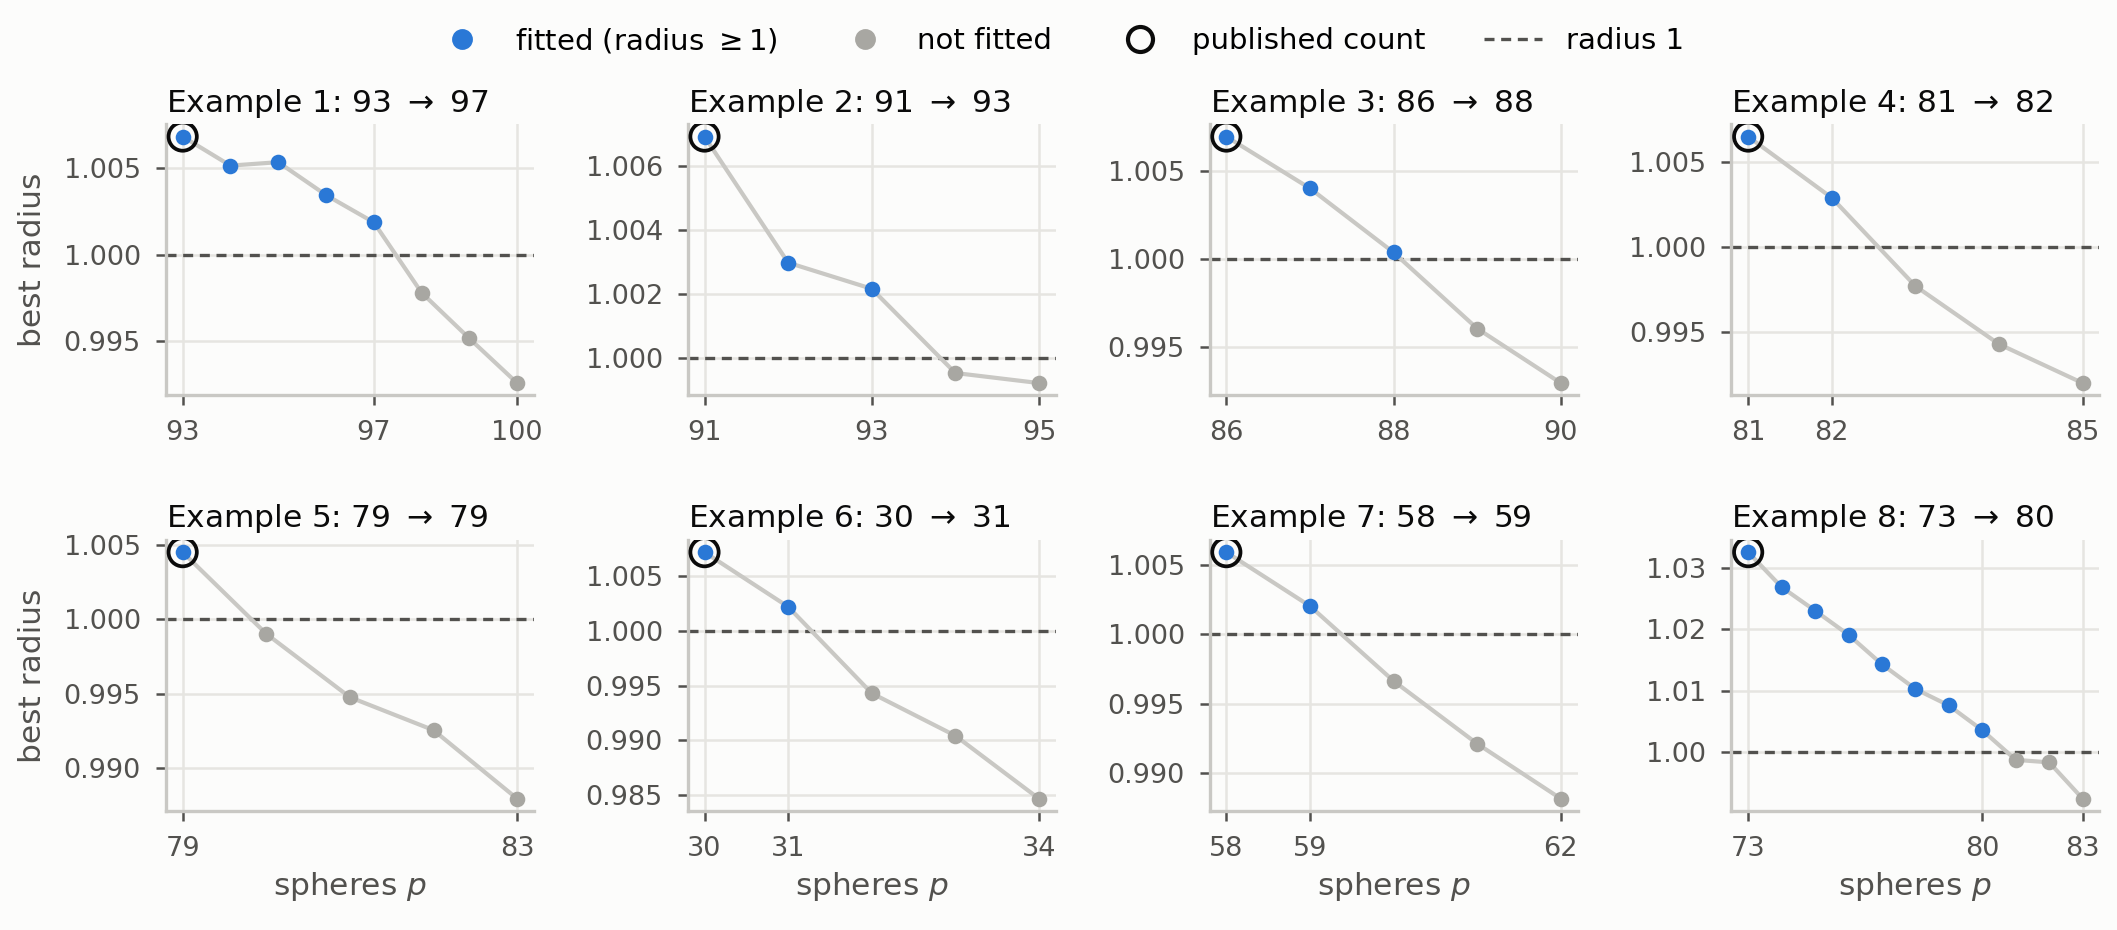
\includegraphics[width=\textwidth]{figures/stoyan_yaskov.png}
  \caption{Best certified radius over 10 seeds at each sphere count tried, in
    the eight domains of \citet{stoyan2013}, under $\ell_2$. A count is fitted
    (blue) when the radius reaches one (dashed); the ring marks their
    published count, and the panel title gives their count and ours.}
  \label{fig:stoyan}
\end{figure*}

\begin{rvdraft}
The domain of example 6 shows why the escape step is needed. The cuboid
there is pierced by a tapered hole whose floor leaves a wall below it, $1.97$
thick at one end and $1$ at the other. A sphere that ends in that wall,
against the end face, the bottom and the sloping floor of the hole, can have
radius at most $0.93364$, the inradius of that wedge. Without the escape
step, 8 of the 10 seeds at every count stopped at exactly this radius: a
restart at the best radius found so far is already feasible there, so Tabu
Search never has to move the trapped sphere. \tbdtext{with the escape step:
how many runs still end with a sphere in the wall, the radii reached, and
our count} (Fig.~\ref{fig:stoyan_ex6}).
\end{rvdraft}

\begin{figure}[t]
  \centering
  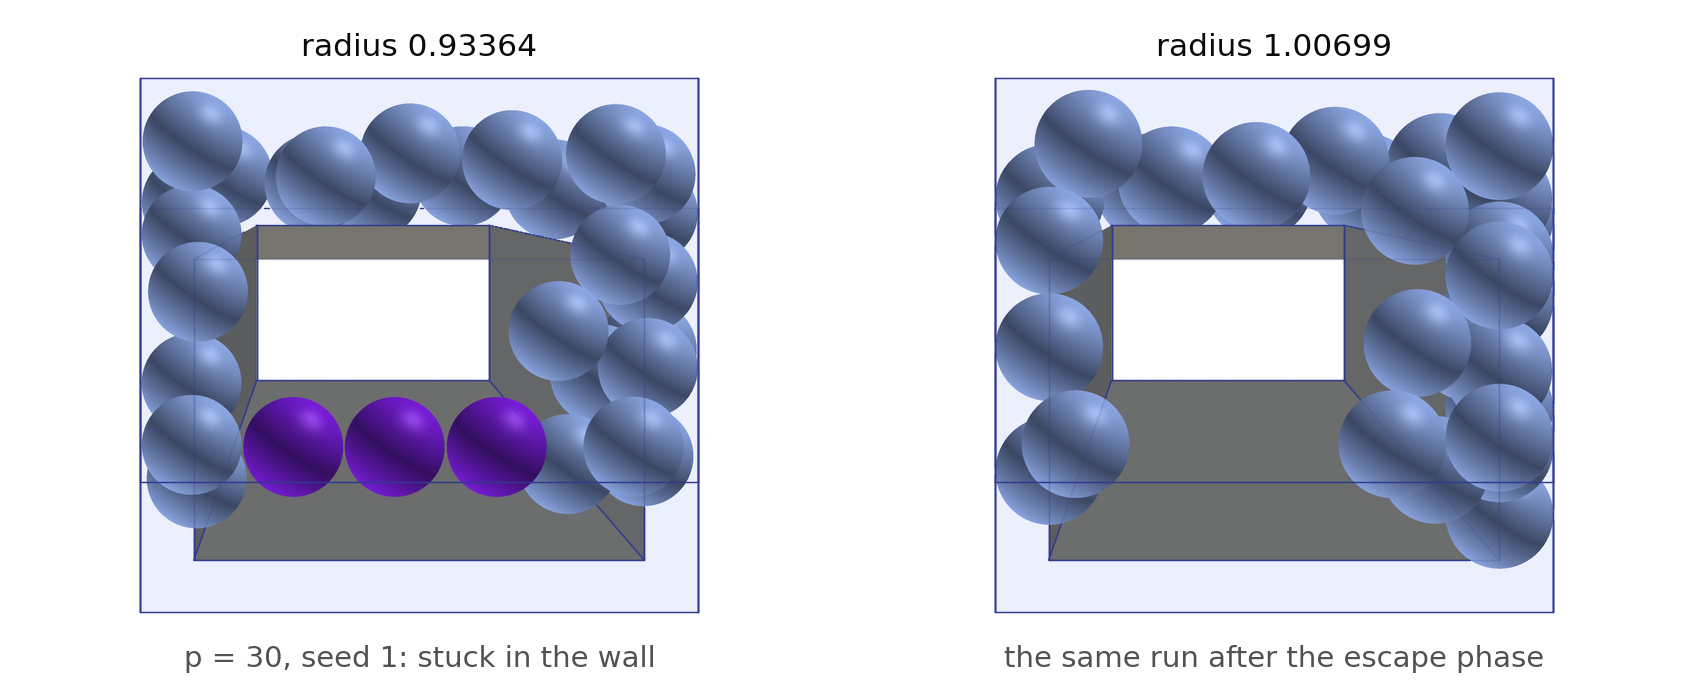
\includegraphics[width=\columnwidth]{figures/stoyan_yaskov_ex6.png}
  \caption{Example 6 of \citet{stoyan2013}, seen end-on along the tapered
    hole (gray; the far opening is white). Left: a run without the escape
    step, with three spheres (purple) in the wall under the hole, which caps
    the radius at $0.93364$. Right: the same seed with the escape step, the
    wall empty and the radius \tbd{1.00699}.}
  \label{fig:stoyan_ex6}
\end{figure}

\begin{rvdraft}
The same domains under $\ell_1$ and $\ell_\infty$ have no published
counterpart, and behave as the volumes of the balls predict: at the
published counts our best radius is \tbd{1.17} to \tbd{1.36} under
$\ell_1$, whose ball is an octahedron, and \tbdtext{whether every count
tried fits}, while under $\ell_\infty$, whose ball is a cube, it is
\tbd{0.85} to \tbd{0.89} and \tbdtext{whether any count fits}.
\end{rvdraft}

\subsection{Comparison with General-Purpose Solvers}\label{sec:baselines}

We also compare our algorithm with general-purpose nonlinear solvers given
the same problem and the same time. The protocol was fixed in writing
before any run, and commits us to reporting every cell, including those we
lose.

\paragraph{Solvers and formulation.} The baselines are IPOPT 3.14, an
interior-point method \citep{wachter2006}, and SLSQP, sequential quadratic
programming \citep{kraft1988, scipy2020}. Each is given the constrained program
$\max D$ subject to $d(c_i, c_j) \ge 2D$ and a clearance of at least $D$ for
every point, formulated as a practitioner would pose it. Dispersion is
$\norm{c_i - c_j}_2^2 \ge 4D^2$ under $\ell_2$; under $\ell_1$ and
$\ell_\infty$, whose norms are not differentiable, it uses a smooth
approximation of width $10^{-6}$ times the container's extent. On the convex
containers, containment is one exact linear constraint per face,
$\ang{n_f, c_i - P_f} \ge D \norm{n_f}_*$. On the non-convex ones it is a signed
clearance oracle, the exact distance to the boundary inside and its negative
outside, with an analytic gradient, so that a solver always has a direction
back into the container. Both solvers receive analytic Jacobians, are
restarted from random configurations until their budget ends, and never see
our energy model or search.

\paragraph{Budget and cells.} The 45 cells are every container and metric at
$p \in \set{10, 20, 40}$. Each solver makes 10 trials per cell, one core each,
and every trial on a cell receives the same wall time,
$\max \set{60\,\text{s},\ 2 t_{\text{med}}}$, where $t_{\text{med}}$ is our
algorithm's median run time on that cell in the main experiment. A start or
local solve still running when the budget ends does not count. Every radius,
for every solver, is scored as certified by the bound $B(X)$ of
Equation~\ref{eq:bound}.

\begin{rvdraft}
\paragraph{Quality.} At equal time our algorithm finds a larger radius
(best of 10) than IPOPT in \tbd{32} of the 45 cells and than SLSQP in
\tbd{25}, and ties the rest to within $10^{-6}$ (relative) \tbdcheck. A
two-sided Wilcoxon signed-rank test on the paired best radii gives
$p = \tbd{1.1e-13}$ against IPOPT and $p = \tbd{3.3e-4}$ against SLSQP.
\tbdtext{how the advantage depends on the geometry: convex containers at
$p = 10$, $20$, $40$, and the largest margins on the non-convex ones}
(Fig.~\ref{fig:baseline_quality}).
\end{rvdraft}

\begin{figure*}[t]
  \centering
  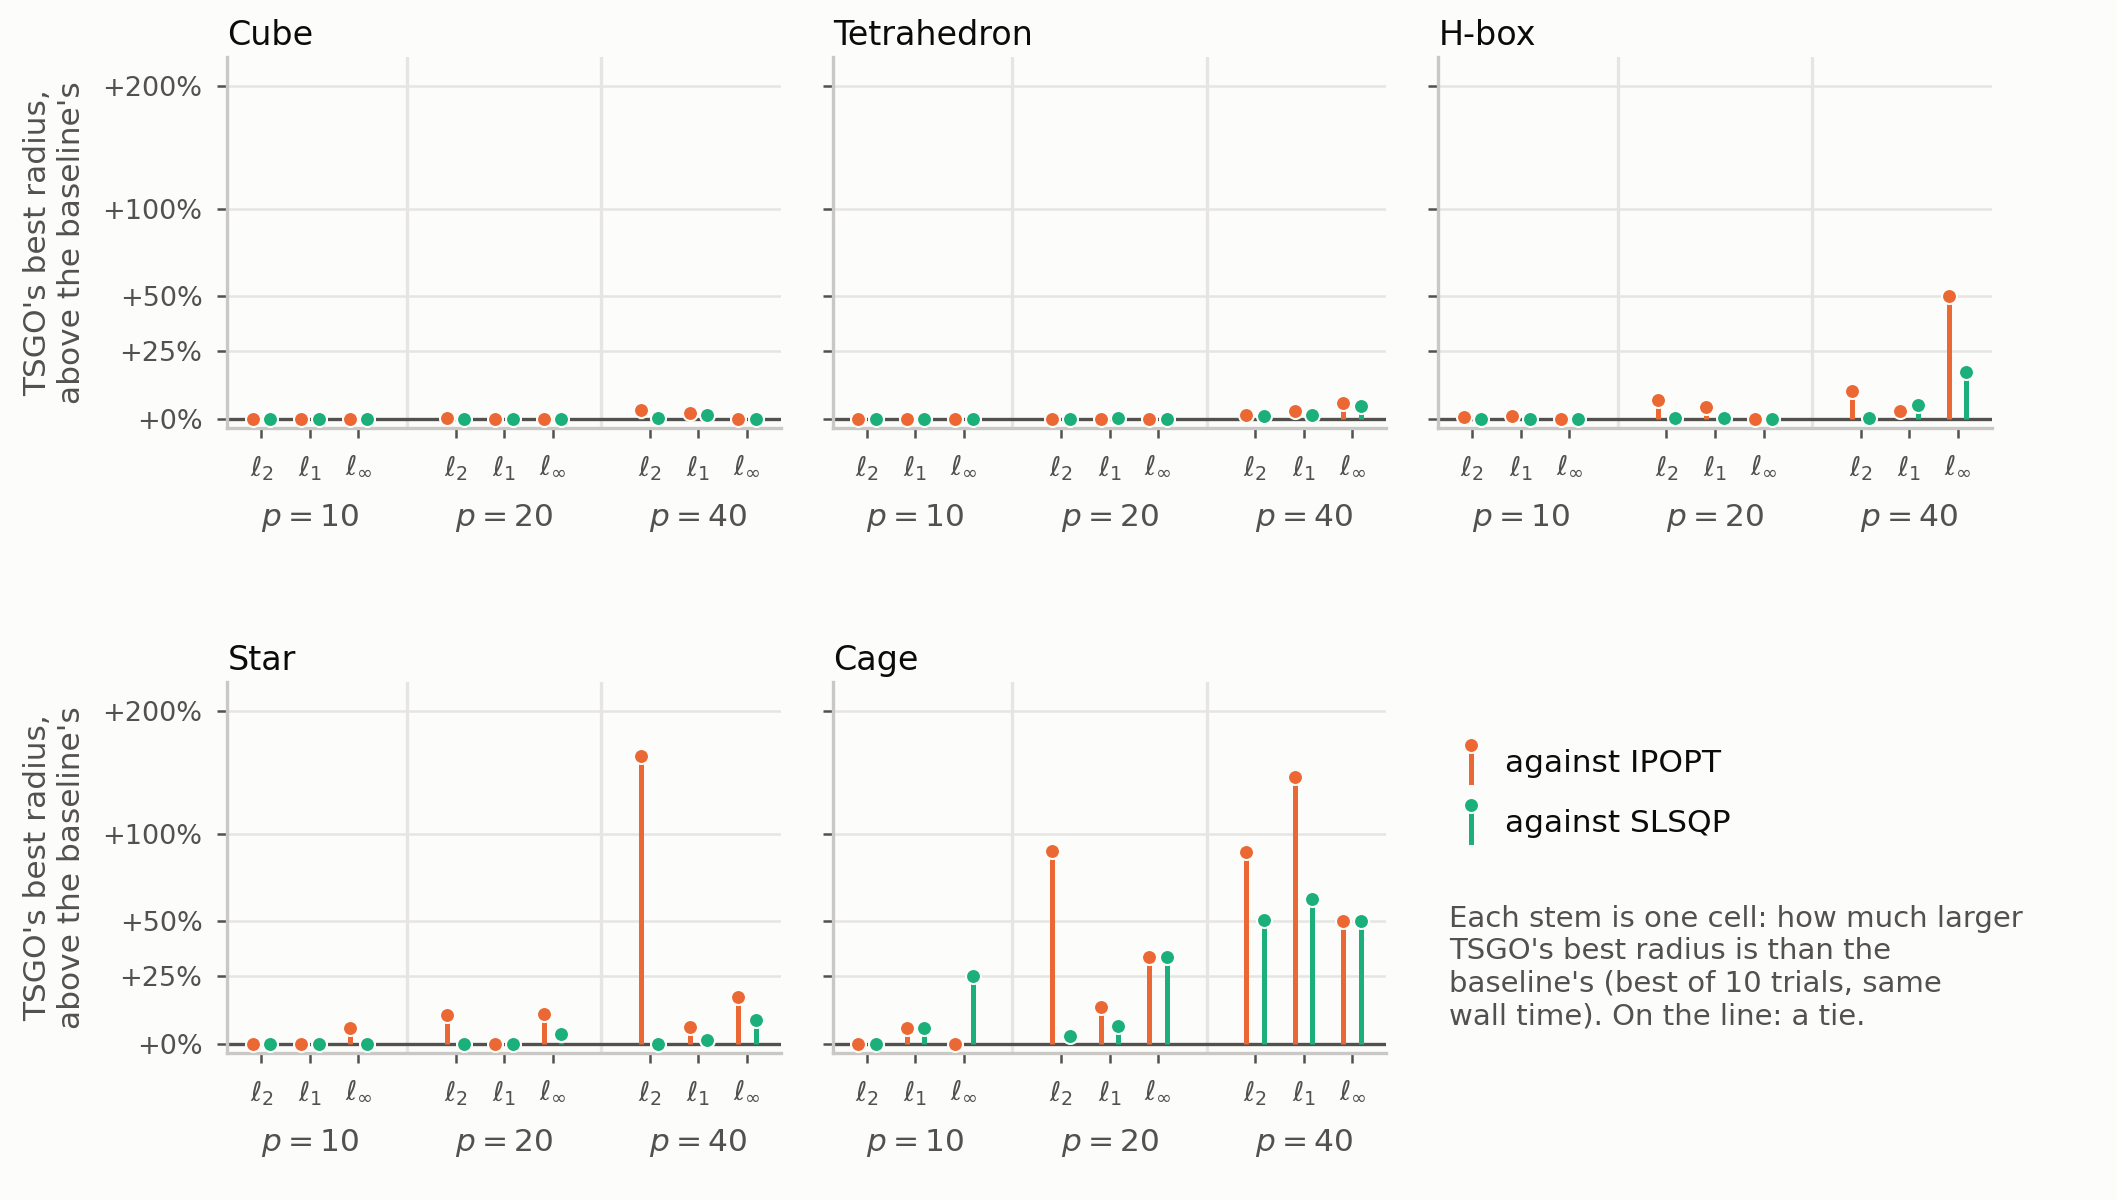
\includegraphics[width=\textwidth]{figures/baseline_quality.png}
  \caption{How much larger our best radius is than each baseline's, in every
    cell: best of 10 trials at equal wall time. One stem per cell and baseline
    (IPOPT orange, SLSQP green); a stem's height is our advantage, and a dot on
    the line is a tie. Within each panel the cells run $p = 10, 20, 40$, and
    within each $p$ the three metrics. The vertical scale is logarithmic.}
  \label{fig:baseline_quality}
\end{figure*}

\begin{rvdraft}
\paragraph{Speed.} \tbdtext{in the cells all three solvers solve, how much
sooner the median trial of each baseline reaches $99.9\%$ of the best
radius found; in how many of our 450 trials the first start was still
running when the budget ended; in how many cells only our algorithm reaches
the target in most trials, and in how many no solver does; how many cells
each solver reaches the target in, and is first in}
(Fig.~\ref{fig:baseline_profile}). Fig.~\ref{fig:baseline_anytime} shows the
progress over time on four hard cells \tbdtext{pattern}.
\end{rvdraft}

\begin{figure*}[t]
  \centering
  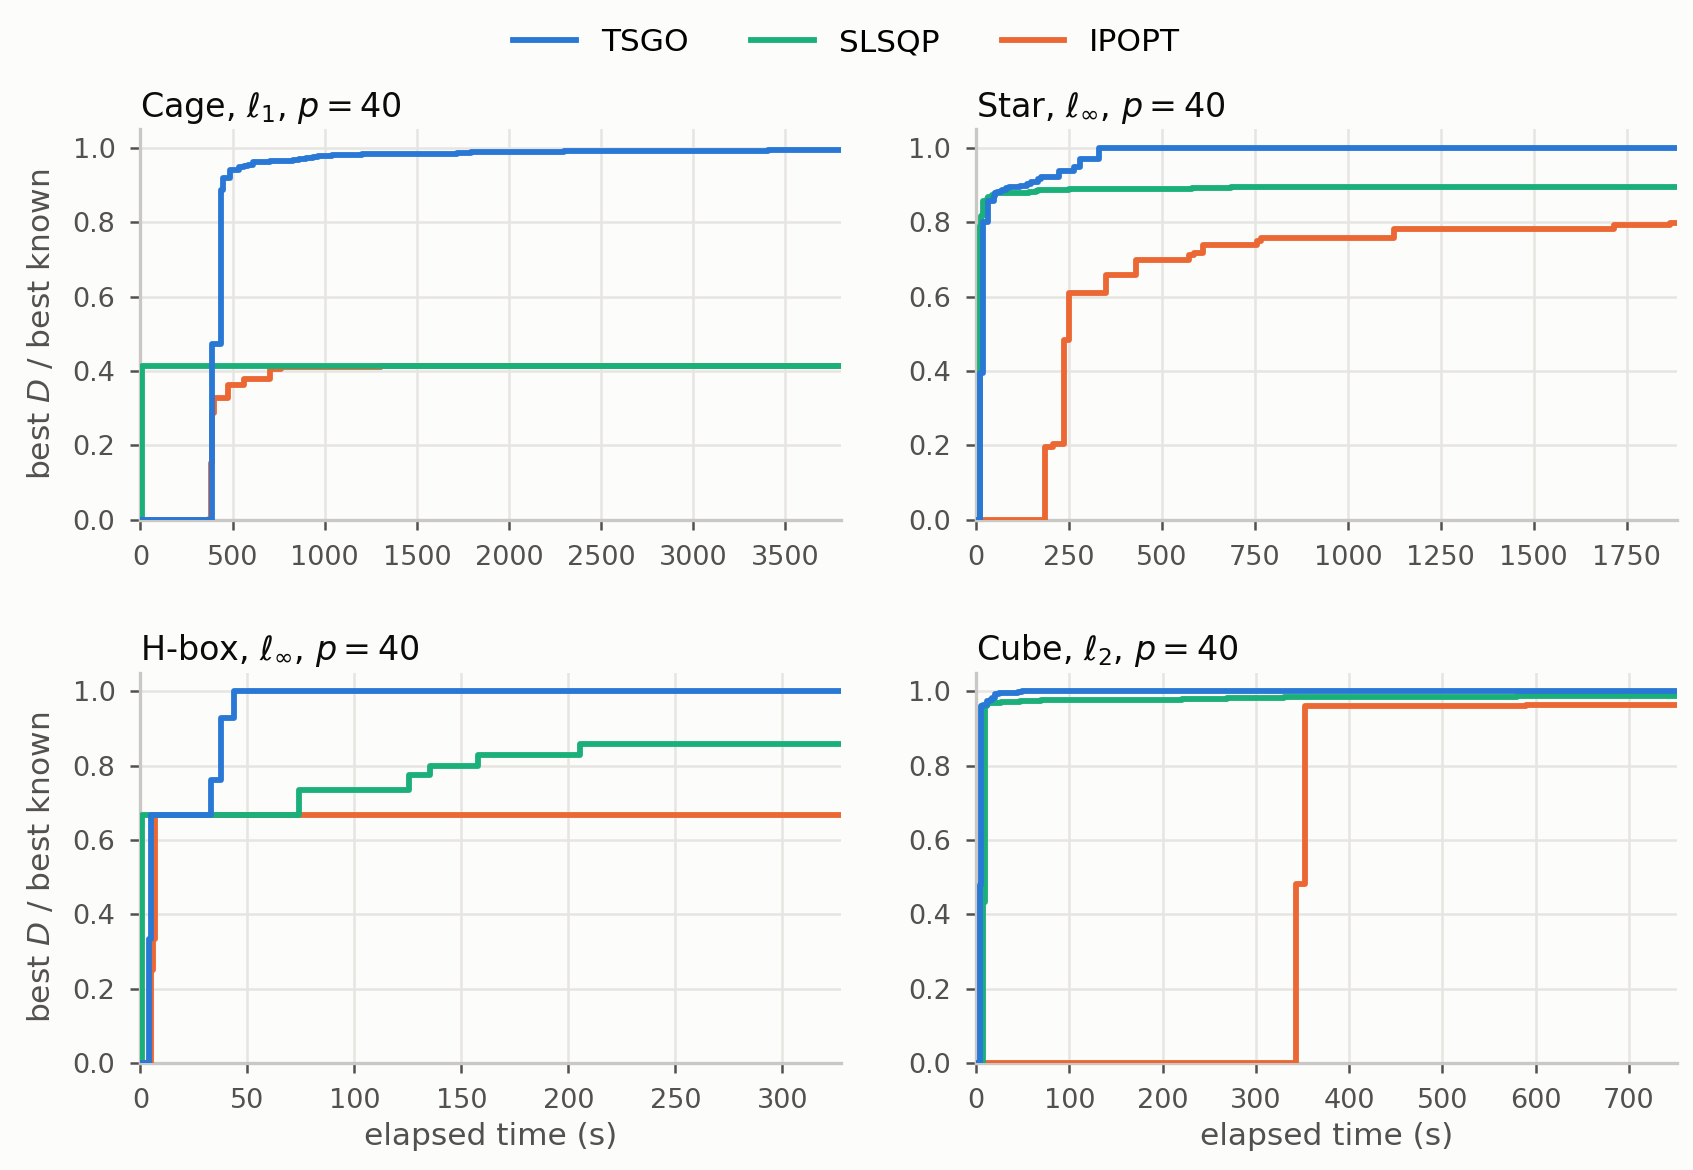
\includegraphics[width=0.8\textwidth]{figures/baseline_anytime.png}
  \caption{Best certified radius against elapsed time on four hard cells, as
    a fraction of the best radius known on the cell (Packomania for the cube);
    median over 10 trials.}
  \label{fig:baseline_anytime}
\end{figure*}

\begin{figure*}[t]
  \centering
  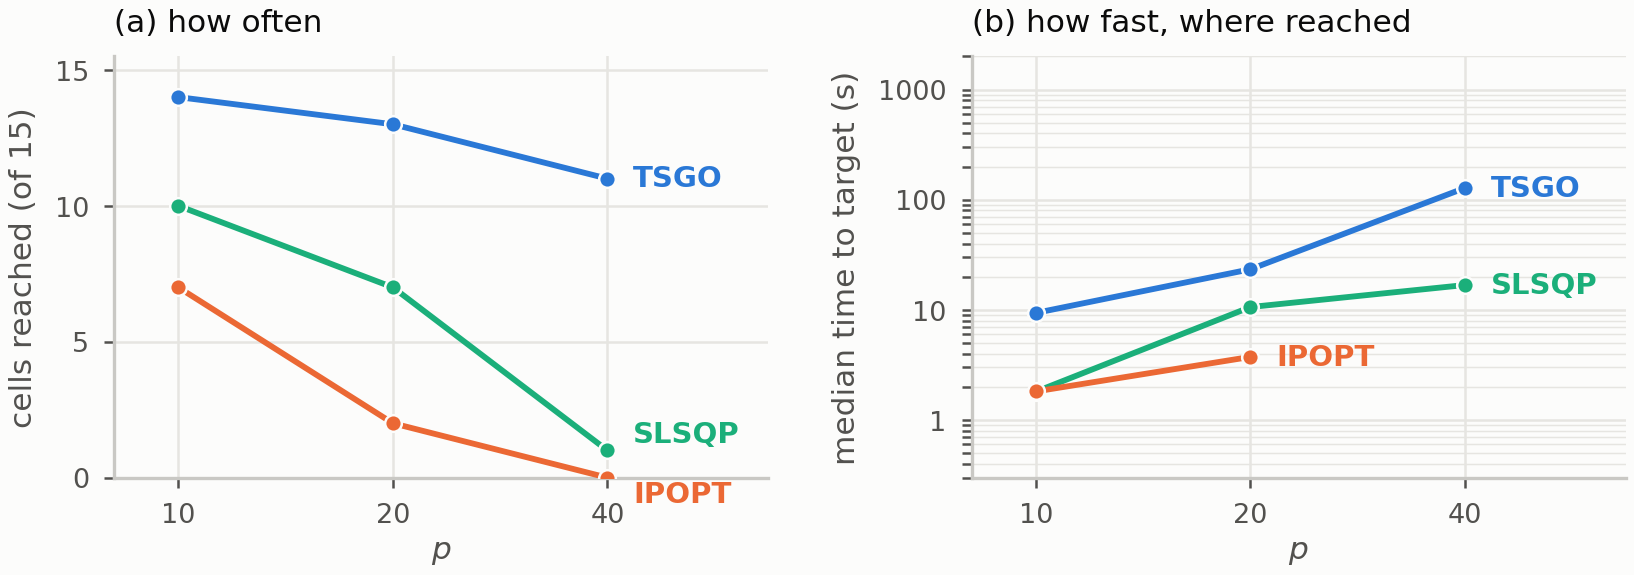
\includegraphics[width=0.8\textwidth]{figures/baseline_reach.png}
  \caption{Reaching $99.9\%$ of the best radius found, judged by each solver's
    median trial, over the 15 cells (five containers, three metrics) at each
    $p$ of the comparison panel. (a) The number of cells in which the median
    trial reaches the target within the budget. (b) The median time it takes,
    over those cells only; a solver with no such cell at some $p$ has no point
    there.}
  \label{fig:baseline_profile}
\end{figure*}

\begin{rvdraft}
\paragraph{Feasibility of reported radii.} A local solver stops when its
constraint violation falls below a tolerance, so the radius it reports can
exceed the radius its configuration supports. Of SLSQP's converged local
solves, \tbd{36.5}\% overstate the radius by more than $10^{-6}$ (relative),
\tbd{0.9}\% by more than $1\%$, and \tbd{1.0}\% report convergence on a
configuration that supports no positive radius at all. For IPOPT the shares
are \tbd{18.3}\% and \tbd{under 0.01}\%. Every radius in this comparison, for every solver, is therefore
the certified $B(X)$; our algorithm reports $B(X)$ by construction.
\end{rvdraft}

\begin{rvdraft}
\paragraph{Optimality.} For the convex containers under $\ell_2$, Gurobi's
spatial branch-and-bound \citep{gurobi2026}, warm-started from our best
configuration, closes its optimality gap within one hour for the cube with
$p \le 9$ and the tetrahedron with $p \le 10$. In every one of these cases
our radius is within $1.5 \times 10^{-5}$ of Gurobi's bound \tbdcheck, which
is the
resolution of Gurobi's constraint tolerance. For the cube at $p = 10$, where
Gurobi does not close its gap in an hour, Packomania records a proven optimum
of $3/14$, which our radius matches to the relative $10^{-9}$ by which every
reported radius is shrunk \tbdcheck. On the tetrahedron at $p = 10$ the proven optimum
is $0.112372$; the benchmark of \citet{kazakov2018}, $0.102$, is $9.2\%$ below
it.
\end{rvdraft}

\begin{rvdraft}
Gurobi also entered the equal-budget comparison on the six cells it can model
(cube and tetrahedron, $\ell_2$, $p = 10, 20, 40$), on one core per trial like
the other solvers, scored by the certified radius of its best incumbent.
\tbdtext{in which of the six cells Gurobi ties our algorithm and by how much
it is behind in the others}; at $p = 20$ our algorithm reaches the radius of
the stacked tetrahedral arrangement, $1/(6 + 2\sqrt6)$ \tbdcheck.
\end{rvdraft}

\subsection{Computational Efficiency and Scalability}\label{sec:runtime}

\begin{rvdraft}
To evaluate scalability, we recorded the wall-clock time of every run, all
of its starts and any fallback attempts included ($\epsilon = 10^{-8}$).
Fig.~\ref{fig:combined_runtime} plots, for every container and $p$, the mean
over the twenty runs of a cell on logarithmic axes, where a power law is a
straight line and its exponent is the slope.
\end{rvdraft}

\begin{figure*}[t]
  \centering
  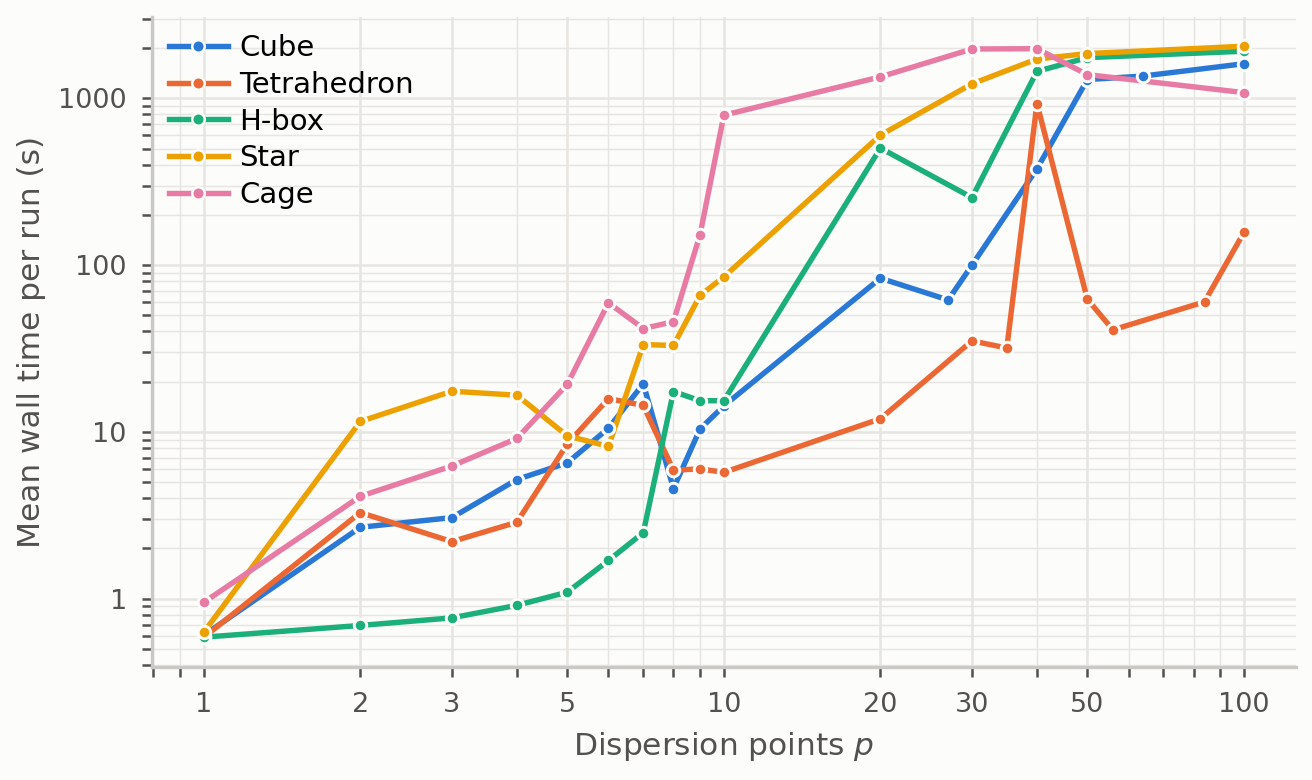
\includegraphics[width=0.62\textwidth]{figures/runtime_euclidean.png}
  \caption{\textbf{Mean solve time per run, Euclidean metric.} Each point is
    the mean wall-clock time over the seeds of one cell; both axes are
    logarithmic. The ribbed cage is included but does not scale with $p$; see
  the text.}
  \label{fig:combined_runtime}
\end{figure*}

\begin{rvdraft}
The 30-minute limit, which includes the escape attempts, shapes the right
of the plot. It ended \tbd{599} of the \tbd{4,800} runs, \tbdtext{at which
$p$}, so the mean times there measure the limit as much as the algorithm.
Fitting $\log t$ against $\log p$ over $p \ge 10$ gives exponents of
\tbd{2.32} for the cube ($R^2 = \tbd{0.90}$) and \tbd{2.06} for the H-box
($R^2 = \tbd{0.78}$), consistent with the $\mathcal{O}(p^2)$ pairwise
distance checks and the $\mathcal{O}(p M)$ boundary checks, where $M$ is
the number of faces. \tbdtext{exponents and $R^2$ for the star, the
tetrahedron and the cage, and which of them do not follow a power law}
\end{rvdraft}

\begin{rvdraft}
No container shows growth faster than polynomial up to the limit
\tbdcheck. The slowest cell, \tbdtext{which}, averages \tbd{2,121} seconds
per run: its runs reach the limit and then finish the restart under way.
\end{rvdraft}

\section{Conclusion}

\begin{rvdraft}
This paper presents a global optimization algorithm for the Continuous
$p$-Dispersion Problem (CpDP) in three-dimensional polyhedral containers
under any norm-induced metric. It extends the Tabu Search approach of
\citet{lai2024} with an almost-everywhere differentiable
feasibility-residual function, distances to the faces, edges and vertices of
the container that are exact for every norm, and a ray-casting test for
whether a point lies in the container. Our method matches the proven optima
and best-known values in the unit cube \cite{schaer1966, packomania}
\tbdcheck; reaches the optima Gurobi certifies in the regular tetrahedron
\tbdcheck, which the grid-based values of \citet{kazakov2018} miss by up
to $9.2\%$; packs more spheres than published in \tbd{seven} of the eight
multi-connected domains of \citet{stoyan2013}; and, at equal wall time,
finds a larger radius than IPOPT in \tbd{32} of 45 cells and than SLSQP in
\tbd{25}, tying the rest \tbdcheck. It also sets benchmarks for three
non-convex containers of our own design, with every configuration's centers
published alongside a script that checks them, for applications such as
robotic collision avoidance and facility layout
\cite{abdulghafoor2021, loganathan2024}.
\end{rvdraft}

\begin{rvdraft}
Restarting at the best radius has a blind spot: a random start already
feasible at that radius is not moved. The escape step of
Section~\ref{sec:global} removes it by aiming Tabu Search slightly above the
best radius whenever a restart gains nothing. \tbdtext{its effect across the
benchmark, from the sweep}
\end{rvdraft}

Because our energy formulation relies on dimension-independent vector
operations, it provides a natural foundation for extension into
$n$-dimensional spaces ($\mathbb{R}^n$). The primary adaptation
required for higher dimensions is generalizing the geometric
container representation, specifically determining how to precisely
model $(n-1)$-dimensional bounding hyperplanes and extending the
ray-casting validity checks. Furthermore, future work will focus on
incorporating more sophisticated, non-planar geometries such as
curved surfaces. Distances to polyhedral boundaries have closed forms:
orthogonal projection in the Euclidean case, and a finite search over the
vertices of the dual unit ball for a polyhedral norm. Curved boundaries
require representations like spline patches or implicit surfaces,
necessitating the development of computationally efficient distance
evaluation methods that do not rely on closed-form projections.

\pagebreak

\begin{widetext}
  \section*{CRediT authorship contribution statement}
  \textbf{Sanjay Manoj:} Conceptualization, Software, Writing -- original
  draft. \textbf{Melkior Ornik:} Conceptualization, Supervision, Writing --
  review \& editing.

  \section*{Acknowledgements}
  The authors would like to thank Ram Padmanabhan for their valuable
  feedback and editorial assistance throughout the preparation of
  this manuscript.

  \section*{Funding}
  This research did not receive any specific grant from funding agencies
  in the public, commercial, or not-for-profit sectors.

  \section*{Data availability}
  The source code, the centers of every configuration reported in this
  paper, and a standalone script that verifies them are available at
  \url{https://github.com/leadcatlab/continuous-p-dispersion}.

  \section*{Declaration of generative AI and AI-assisted technologies in
  the writing process}
  During the preparation of this work the authors used Claude Opus 5.5
  (Anthropic) to find speed-ups in the implementation of the algorithm, to
  check proofs, and to draft parts of the text. After using this tool, the
  authors reviewed and edited the content as needed and take full
  responsibility for the content of the publication.
\end{widetext}

\bibliographystyle{unsrtnat}
\bibliography{continuous-p-dispersion-in-three-dimensions}

\end{document}
